%
% Tissue Clonal Selection
% Jason Brownlee
%
\chapter{Tissue Clonal Selection}
\label{chap:tissues}

%
% Overview 
% Provides an overview of the chapter and its structure, and a description of what is intended to be achieved by providing this documentation. A description of why and how this chapter follows on from the previous chapter
%
\section{Chapter Overview}
\label{sec:tissues:overview}
% this chapter
This chapter exploits the principles and findings of the cellular paradigm by taking them for granted, instead investigating clonal selection where the cellular paradigm is a primitive component in a broader \emph{Tissue Clonal Selection Paradigm}. 
% biology
Section~\ref{sec:tissues:migration} reviews the acquired immune system from the perspective of the tissues that provide the structure and manage the function of the lymphocytes central to the clonal selection theory. 
% abstraction
Section~\ref{sec:tissues:paradigm} considers an abstraction of the reviewed physiology and tissue-based immunology and the basis of the tissue paradigm. Most importantly in this abstraction are the spatial and temporal considerations of the discrete exposure of repertoires of cells to information, and the tissue architectures that provide base patterns for the design of inspired algorithms and implementations.
% realisation
The paradigm is realised as the investigation of Tissue Clonal Selection Algorithms in the context of an Infection Antigenic Exposure Problem, that provides the basis for empirical investigation in the remainder of the chapter. Tissue-based immunology strategies for organising information are defined and empirically investigated in an colour space specialisation of the infection problem, resulting in a series of algorithms: the Minimal, Recirculation, Homing, and Inflammation Tissue Clonal Selection Algorithms. 
% findings
The investigation of these algorithms confirms expectations regarding the natural organisation of information based on the regularity and consistency of exposure, as well as important findings as to how the defined strategies may be exploited when such regularities and consistencies are not known \emph{a priori}.

%
% Physiology of Lymphocyte Migration
%
\section{Physiology of Lymphocyte Migration}
\label{sec:tissues:migration}
The white blood cells and immunoglobulin within a host that comprise the recognition and response component of the acquired immune system are \emph{mobile}. There are pools of lymphocytes that recirculate the blood stream and the lymphatic system. More interestingly there are lymphocytes that selectively home to tissues close to where the cells were created and there are pools lymphocytes that are recruited to sites of infection and inflammation. The lymphoid tissue of the lymphatic system provides the structural scaffold for the mobility of these cells and related molecules, although interestingly the migratory behaviour is controlled at the finest level: through localised molecules and receptors on the cells themselves. The migration of cells involved in the immune system is highly complex and is still not completely understood. This section reviews some superficial features of lymphocyte migration in the immune system with the interest of extracting principles for use in clonal selection-based Artificial Immune Systems. Lymphocyte migration is reviewed in the context of the human and related mammalian immune systems, providing perspectives of cell movements from the lymphatic system, movement types, cell types, and cell classes. 

%
% Lymphatic System
%
\subsection{Lymphatic System}
\label{subsec:tissues:migration:lymphatic}
The lymphatic system is a complex collection of lymphoid organs integrally related to the functioning of the immune system and responsible for the transport and filtering. Lymph is a clear bodily fluid that surrounds all tissue that forms when proteins and cells leak out of blood carrying venules and capillaries. The lymph carrying capillaries flow uni-directionally draining the lymph back to lymphoid tissues that make up the lymphatic system. Also carried in this lymph are antigens that may have entered the organism. The lymphatic system acts as a secondary circulation system (to the cardiovascular circulatory system) transporting lymphocytes between lymphoid organs, and carrying antigen to lymphoid organs for interaction with lymphocytes. There are two types of lymphoid organs (1) the primary or central tissues which are the sites of lymphocyte formation (the thymus and bone marrow), and (2) the secondary or periphery lymphoid organs where immune response take place (the spleen, lymph nodes and gut-associated lymphoid tissues). One may consider the rest of the bodies' tissues as tertiary lymphoid tissues which normally only contain few lymphoid cells, although on infection and inflammation, manage to recruit many immune cells.

%
% Central Lymphoid Tissues
%
\subsubsection{Central Lymphoid Tissues}
Primary lymphoid organs consist of the thymus and the bone marrow, and are responsible for differentiating stem cells into pre-immune cells (pre-B-cells and pre-T-cells) in a process that is believed to be independent of antigenic stimulation. The bone marrow provides a micro-environment for the production of blood cells. B-cells migrate to secondary lymphoid organs, whereas T-cells migrate to the thymus. The thymus provides an environment for the further antigen-free maturation of T-lymphocytes. Cells proliferate and differentiate in a process involving negative and positive selection where the majority of produced T-cells never leave the thymus. Those cells that do survive (less than 5\% per day) may join the recirculating lymphocyte pool, or migrate to secondary lymphoid tissues. There are two types of of primary lymphoid tissues, as follows:

\begin{itemize}
	\item \emph{Bone Marrow}: Tissue located inside large bones responsible for the production of many different blood cell types not limited to lymphocytes (white blood cells). Provides an environment for differentiation of \naive\ B-cells.
	\item \emph{Thymus}: An organ located behind the sternum, providing an environment for the differentiation of \naive\ lymphocytes from bone marrow. These lymphocytes differentiate into T-lymphocytes, which involves a negative selection maturation process.
\end{itemize}

% 
% Peripheral Lymphoid Tissues
% 
\subsubsection{Peripheral Lymphoid Tissues}
The secondary lymphoid tissue is responsible for collecting antigens at points in the organism where they may enter, and facilitate their exposure to recirculating lymphocytes. For example, the lymph nodes are primarily responsible for filtering the lymph for antigens, the spleen is responsible for filtering the blood for antigens, and the tonsils for the respiratory system. Goodnow puts this concisely suggesting that the ``\emph{\ldots central function of secondary lymphoid tissues is filtering: collecting blood-borne, lymph-borne, or mucus membrane antigens and holding these so that they can be surveyed by immune cells before being destroyed}'' \cite{Goodnow1997} (page 6). The secondary lymphoid organs are as follows:

\begin{itemize}
	\item \emph{Tonsils}: A collection of lymphoid tissue on the side of the throat responsible for providing lymphocyte access to and protection of the respiratory system from antigen.
	\item \emph{Lymph Nodes}: Small gland like structures found throughout the body that filter the lymph for foreign antigen material, which are then presented to lymphocytes and other immune system cells.
	\item \emph{Peyer's Patches}: A collection of lymphoid tissue found in the lowest section of the small intestine. There are numerous instances of these patches in the intestine and they act like lymph nodes, and provide centres for lymphocytes protecting the gastrointestinal tract.
	\item \emph{Spleen}: An organ in the upper abdomen, responsible for the destruction of old red blood cells. It is the only lymphoid organ that crosses the blood stream, and thus provides a site where lymphocytes can interact with antigens carried in the blood.
	\item \emph{Lymphatic vessels}: Vessels throughout the body that carry lymph. They are responsible for transporting lymph from tissues to the blood (vascular circulatory system) and to the lymph organs.
\end{itemize}

In addition, the secondary lymphoid tissue provides a suitable micro-environment for the development and maturation of an immune response, such as the formation of Germinal Centres (GC's) for B-cell clonal expansion and affinity maturation. Germinal Centres are little understood dynamically generated regions in lymphoid tissue where activated B-lymphocytes clonally expand, undergo hypermutation, and ultimately differentiate into plasma and long-lived memory B-lymphocytes \cite{Berek1991, Thorbecke1994}. GC's are founded by a small number of activated B-cells (oligoclonal), which are in turn co-stimulated by helper T-cells \cite{Liu1997}. It is believed that there are repeated rounds of selection, expansion, and mutation of B-cells within the GC. The majority of the produced B-cells may be plasma cells and have a lower affinity than the founding cells, although a few higher affinity clones are preferentially selected to survive as plasma or memory cells \cite{MacLennan1994, Meyer-Hermann2005}. Those cells that are worse die due to the lack of positive selection. GC-like structures may also occur outside of lymph nodes, such as sites of infection and allergic inflammation \cite{Gould2006}.

The geography of the lymph nodes and other secondary lymphoid tissues plays an important structural role for lymphocyte selection and response, for example Zinkernagel, et~al. suggests that the ``\emph{\ldots secondary lymphoid organs present antigen optimally and enhance the chances of specific antigen encounter and specific cell interactions.''} and that ``\emph{\ldots these requirements render chance encounters of antigen by lymphocytes and activation elsewhere extremely inefficient and of no biological relevance.}'' \cite{Zinkernagel1997} (page 201). It is likely that the organisation and function of the secondary lymphoid organs has been optimised for recirculating lymphocytes to efficiently detect and remove pathogens from the organism, for example Fu and Chaplin suggest that ``\emph{\ldots secondary lymphoid organs are thought to be organised into structures that optimize cellular interactions that support the efficient removal of unwanted pathogens}'' \cite{Fu1999} (page 400). Finally, in addition to providing a scaffold for lymphocyte recirculation, the secondary lymphoid tissues possess a high regenerative capacity. When circulation routes are disrupted or severed, the tissue is able to adaptively regenerate a connection between the effected nodes \cite{Olszewski2003}. 

%
% Summary
% Lymphatic Perspective of Mobility
%
\subsubsection{Summary}
There are no lymphocytes or lymphocyte recirculation without the lymphatic system. The tissues are responsible for the development and management of the cells throughout their life cycle. The following summarises the lymphatic system's governing role over lymphocytes:

\begin{enumerate}
	\item \emph{Formation}: Provide an optimal micro-environment for the production and maturation of lymphocytes. 
	\item \emph{Presentation}: Collect diverse populations of lymphocytes into organ systems that drain antigens from entry points into the organism.
	\item \emph{Regulation}: Regulate interactions of different classes of lymphocytes in drainage organ systems, such as the arrangement of B-cells and T-cells.
	\item \emph{Dissemination}: Disburse effector elements of the immune response throughout the organism, and disseminate and amplify the immune response systematically throughout the lymphatic system.
\end{enumerate}

For more information regarding the anatomy and physiology of the human lymphoid system see any current anatomy and physiology text on the subject, such as \cite{Marieb2006}. Other references used include lymphoid organ summaries by de~Castro and Timmis \cite{Castro2002a} (page 71), Anderson \cite{Anderson1990a}, and Swartz \cite{Swartz2001}. See Andrian and Mempel for a review of lymph node anatomy and physiology in the context of cell migration \cite{Andrian2003}.

%
% Lymphocyte Mobility
% 
\subsection{Lymphocyte Mobility}
\label{subsec:tissues:migration:mobility}
Cell movement is the basis of immunology. It is involved in inflammation, differentiation, adhesion, recruitment, and required for cellular and molecular interactions. The recirculation of lymphocytes was confirmed experimentally almost 50 years ago by Gowans and colleagues \cite{Gowans1959, Gowans1964}, although the study of the topic is often neglected in favour of cell interactions \cite{Young1999a, Perelson1997}. Interestingly much of the modelling work with populations of lymphocytes does not take into account the spatial heterogeneity of the lymphatic system. 

The adhesion properties of cells plays a critical controlling role in the movement of lymphocytes (see Anderson for a treatment \cite{Anderson1990a}). Adhesion is used by cells to crawl through tissues, and is used by activated cells to stick to the molecule that activated them. Adhesive receptors (so-called `homing receptors') and chemicals are little understood and are a topic for intense study. The adhesive characteristics of a cell are believed to be selected for and differentiated along with cell antigenic receptor characteristics. These adhesive interactions provide bottom up control at the finest level \cite{Picker1992}, believed to be the basis for homing, recruitment and may ultimately control the extent and scope of the immune response \cite{Warnock1998}. A procedure or series of adhesive-based decisions have to be made for a lymphocyte to be recruited into tissues, in particular from recirculation in the blood into lymphoid tissues. This process is called the multi-step extravasation or molecular regulation procedure, which has the following four steps: (1) primary cell adhesion, (2) rapid cell activation, (3) activation dependant arrest, and (4) diapedesis (the movement into surrounding tissue).

%
% Movement Types
%
\subsubsection{Movement Types}
\label{subsubsec:tissues:migration:mobility:movement}
Physically, there are two ways lymphocyte cells can move: \emph{crawling} on tissues and \emph{flowing} between tissues. In crawling, cells use chemical receptors to adhere to their surroundings and use this method to slowly migrate through tissues, a place where they spend most of their time given the slow pace of movement. The second mode is movement in fluid space such as in blood or lymph where cells are capable of moving a lot faster, covering great distances within the organism. The process of lymphocyte migration was originally considered to be random, although it is now known that this is not necessarily the case. Lymphocytes may be preferentially recirculated, and are able to home in and target specific tissues. In addition, memory lymphocytes show different migration behaviour to \naive\ lymphocytes. For example, memory T-cells preferentially migrate to non-lymphoid tissues. If a memory cell was created in a lymph node near the skin, the cell will preferentially migrate into skin tissue near the lymph node, if created in a lymph node near the gut, it will migrate to neighbouring gut tissue. \Naive\ T-lymphocyte cells are activated by dendritic cells and educated as to the chemical properties of the site of infection. These prepared T-cells recirculate around the host organism in search of their cognate antigen, and upon detecting the chemical properties of the site of infection, home into the tissue. The directed trafficking behaviour is called T-lymphocyte homing \cite{Butcher1999, Butcher1996, Picker1992, Warnock1998}, and the information which controls the where T-cell traffic is expressed as receptors on the surface of the cell for the chemical properties of the site of infection \cite{Ferber2007, Salmi2005}. 

The immune system maintains a pool of recirculating lymphocytes that cycle around the blood and the lymphatic system. The pace of recirculation is high, the number of lymphocytes entering the blood from the lymph each day is 10 times the size of the recirculating lymphocyte pool \cite{Anderson1990a}. The number of lymphocytes recirculating at one time may be anywhere from 1\%-2\% of all lymphocytes in the body in young adult animals \cite{Young1999a, Stekel1997}. Lymphocytes may only stay in circulation in the blood for about 30 minutes. Trepel provided a seminal, although outdated extrapolation of the number and distribution of lymphocytes in man \cite{Trepel1974}. Such numbers may be useful for a general guide, as follows: 2.2\% in the circulating blood, 41.3\% in the lymph node and tonsils, 15.2\% in the spleen, 4.3\% in the gut-associated lymphoid tissues, 10.9\% in the thymus, 10.9\% in the bone marrow, and about 15\% in other tissues. One may summarise the primary types of lymphocyte migration, as follows:

\begin{itemize}
	\item \emph{Trafficking}: The directed (non-random) movement of cells from tissues, blood, or lymph. May refer to a cells trafficking route as it homes to a specific region in the body. For example: pre-B-cells and pre-T-cells migrate to secondary lymphoid tissues to further differentiate and mature.
	\item \emph{Recirculation}: The movement of lymphocyte cells around the body from lymphoid tissue, to the blood, to the lymph, and back to lymphoid tissue to repeat the process (circulation or rolling lymphocytes). \Naive\ and memory cells are the main recirculating lymphocyte types. 
	\item \emph{Recruitment}: Accumulation (sequestration) of cells such as a site of infection or tissue damage, such accumulation may occur through chemotaxis (directed movement in response to a chemical gradient). 
	\item \emph{Homing}: The directed (preferential tendency) of lymphocytes activated in a particular region of the body, to return to that part of the body (localisation). May refer to the arrival of lymphocyte to lymphoid or non-lymphoid tissue from the blood stream. Also called tissue-selective trafficking. Those cells with a memory of where they were differentiated may localise back to these regions after a period of recirculation.
	\item \emph{Stationary}: These are cells that selectively arrest their movement, or do not move from the location of their differentiation. For example in the recruitment of cells, the differentiation of cells such as plasma B-cells created in germinal centres that release large amounts of antibody, and sentinel effector cells.
\end{itemize}

%
% Lymphocyte Types
%
\subsubsection{Lymphocyte Types}
\label{subsubsec:tissues:migration:mobility:cells}
There are both circulating and non-recirculating populations of B- and T-cells. Although the behaviours of both cell types are tightly interrelated, both have differing migration behaviours during their development and life cycle. The general migratory life cycle of T-lymphocytes is as follows: pre-T-cells migrate from bone marrow to the thymus for maturation, surviving T-cells may migrate to tissues and becomes sentinel cells. Other cells may recirculate and seek activation in secondary lymphoid tissue. Memory T-cells preferentially migrate to non-lymphoid tissues. For B-lymphocytes: pre-B cells migrate from the bone marrow to secondary lymphoid tissues. Some cells will be activated by antigen in the secondary tissue and differentiate into plasma and memory cells. Other cells will be activated and migrate to the spleen before differentiating. 

There is commonality in the development of both B- and T-cells, specifically in terms of the generalised classes of lymphocyte they may differentiate into. These include the classes: \emph{\naive}, \emph{effector}, and \emph{memory}. \Naive\ cells are untested lymphocytes that seek a potential cognate antigen. Effector and memory cells result from the union of \naive\ cells and antigen. Effector cells, such as Helper T-cells and plasma B-cells remain in lymphoid tissue. Memory cells make up the majority of the recirculating pool and continue to circulate between the bloodstream and the lymphatic system, at a higher rate than \naive\ cells. One may define the migratory behaviours of the generalised lymphocyte classes or casts, as follows:

\begin{itemize}
	\item \emph{\Naive\ Lymphocytes}: Recirculate between blood and lymphoid tissue, primarily involved in responding to antigen presented in lymph nodes, differentiating into effector and memory cells. Relatively homogeneous in their recirculating behaviour. \Naive\ cells compete with each other for activation and contribution into the memory recirculating pool.
	\item \emph{Effector Lymphocytes}: Typically do not recirculate, stay at the site of differentiation, such as plasma B-cells, which differentiate from \naive\ B-cells in lymph nodes or the spleen.
	\item \emph{Memory Lymphocytes}: Recirculate around blood and lymphoid tissue, but also extravasate to other non-lymphoid tissues. They are heterogeneous in their recirculation behaviour, with restricted and selective recirculation circuits. They home to areas where they are most likely to encounter, or re-encounter their cognate antigen. The number of memory cells is maintained within a moderate range during adult life.
\end{itemize}

%
% Cell Mobility as a Strategy
%
\subsubsection{Cell Mobility as a Strategy}
\label{subsubsec:tissues:migration:mobility:strategy}
The anatomy and physiology of the immune system may be thought of a defence strategy for the organism, and cell mobility is an integral part of that strategy. Picker and Butcher propose such an evolved strategy where the solution to a complex antigenic environment is ``\emph{\ldots to compartmentalize the principle functions of the lymphoid system into discrete organs and tissues in the body, and to connect and unify these organs through the operation of an elegant system of targeted lymphocyte trafficking and recirculation.}'' \cite{Picker1992} (page 562). Some resources of the immune system are fixed in position and distributed throughout the body such as lymphoid tissues, and so called sentinel T-cells. Draining lymph into lymphoid tissue provides a way to localise antigen. Keeping the majority of the immune responses in movement (the detectors and effectors) provides a patrolling approach to rapidly deploy resources to wherever they are needed. The immune system has to produce many cells to detect unknown antigen, and must collect antigen in such a way that rare detector cells are given a chance to detect them. It must provide a micro-environment for controlled proliferation and differentiation, and disperse effectors to where they are needed. Further, Rosen, et~al. consider a recirculating population as an efficient approach in the context of alternative designs where ``\emph{Recirculation contributes to the efficiency of peripheral immune responses by maximising stochastic probabilities of a productive meeting between antigen and its cognate T-cell receptor}'' \cite{Rosen2003} (page 161). This tissue-recirculation adaptive strategy may be considered to have the following general properties:

\begin{itemize}
	\item \emph{Movement}: Different cells and cell types have differentiated migration potentials (so-called `differential migration'). The lymphatic system provides a pathway, which allows lymphocytes to recirculate between blood, peripheral tissues, and lymph nodes.
	\item \emph{Balance}: The so-called stirring or mixing effect of the recirculating lymphocyte pool facilitates the survival of the fittest, that is the survival of the most appropriate clones in the repertoire. The segregation in the repertoire prevents competition between unrelated lymphocyte subsets. Tissues selectively facilitate the segregation of lymphocytes to where they are needed. Such a balance between recirculation and homing may be critical to lymphocyte homoeostasis \cite{Butcher1996}.
	\item \emph{Coverage}: A repertoire of cells is distributed and rotated in an attempt to expose rare (specialised) cells to as many opportunities for activation as are available. This may be considered the maximisation of coverage, where the rolling population seeks to maximise the probability of specialised cells being exposed to their cognate antigen. Large-scale migration allows a wide repertoire of specific lymphocytes to exist at a very low frequency, yet still function efficiently. An example of this is T-cells. Perhaps one in ten thousand T-cells released from the thymus will have a receptor that can detect a given antigen. This means that statistically at least ten thousand inappropriate cells must encounter an antigen before the right one does \cite{Anderson1990a}. 
	\item \emph{Surveillance}: Lymphocytes may be thought of as patrolling the organism, seeking cognate antigen or recruitment. They may also thought of as monitoring the organism for change to self for self-antigen such as tumours in what is known as \emph{immunosurveillance}.
	\item \emph{Amplification}: Recirculation permits recruitment, the dynamic reallocation (localisation) of specialised resources to locations where they are needed. Further, the system is capable of further specialising the recruited resource and disseminating that information.
	\item \emph{Dissemination}: The pathway provided by the lymphatic system provides a highway to rapidly distribute information such as the immune effector cells, antibodies, and long lived lymphocyte cells that retain a refined memory of an antigenic exposure for a future rapid response.
	\item \emph{Alternative}: It provides a distributed mobile defence strategy and is different to other subsystems of the body such as the nervous system, which is distributed but structurally fixed. Further, if the repertoire did not recirculate then each lymph node would be an isolated (island) repertoire. Thus, each such isolated repertoire would either have to be as large as the entire recirculating pool, or a smaller pool resulting in less antigenic coverage.
\end{itemize}

%
% Problems and Changes to Migration
%
\subsubsection{Problems and Changes to Migration}
\label{subsubsec:tissues:migration:mobility:problems}
The rate and nature of lymphocyte migration does not remain constant, and in fact, it may be desirable in certain circumstance to manipulate the recirculation behaviour of lymphocytes. Alternatively, the recirculating behaviour of lymphocytes that provides a dynamic defence may also facilitate significant problems for the host organism. During an immune response, the lymph nodes may rapidly recruit cells from blood, temporally blocking them from leaving the tissue. This in addition to clonal expansion causes the nodes to swell in size and become sore. This swelling of the glands is a common sign of illness. It highlights the point that when an antigenic stimulus is detected, it has a profound effect on the entire system, affecting production and circulation behaviour of lymphocytes. There are some diseases that disrupt and decrease the migration and homoeostasis of lymphocytes \cite{Anderson1995}, thus it may be desirable for the system to temporally increase the rate of cell migration. Some approaches may include increasing blood flow, increasing the expression of adhesive chemicals, and manipulating the tissues where immune responses take place. Alternatively, there are diseases where it is desirable to decrease the recirculation of lymphocytes. Examples include when tissues are transplanted and autoimmune diseases. In both cases the immune cells seek to destroy healthy tissue, thus strategies focus on affecting the recruitment of cells to these areas.

The lymphatic system may facilitate the spread of disease in the body. For example, cancers and tumour cells are able to spread quickly throughout the lymph nodes of a host. Bacteria can use the lymphatic system to disseminate throughout the body. An example mentioned by Andrian and Mempel is the bacterium \emph{Yersinia pestis} one of the most devastating bacterial pathogen in human history (the cause of the bubonic plague) \cite{Andrian2003}. It manages to get in to tissue through flea bites and moves to the lymphatic system where it proliferates, quickly overwhelming lymph nodes and spreading throughout the body. Additionally widely cited examples include the human immunodeficiency virus (HIV) that can lead to the condition of acquired immunodeficiency syndrome (AIDS), \emph{Mycobacterium} that causes diseases including tuberculosis and leprosy, and the bacterium \emph{Bacillus anthracis} that causes the disease Anthrax.

%
% Abstract Tissue Paradigm
%
\section{Abstract Tissue Paradigm}
\label{sec:tissues:paradigm}
Section~\ref{sec:tissues:migration} demonstrated that the tissues that house lymphocytes govern their life cycle, and that together they form a high-level strategy for partitioning and managing the systems interaction with antigen. This section abstracts and elaborates on this tissue-centric adaptive strategy and proposes a \emph{Tissue Clonal Selection Paradigm} that takes the clonal selection of the Cellular Paradigm for granted, and focuses on the inter-tissue interaction and information sharing provided by bottom-up cell migration mechanisms. 
 
%
% Model Components
%
\subsection{Model Components}
\label{subsec:tissues:paradigm:models}


%
% Architecture Components
%
\subsubsection{Architecture Components}
\label{subsec:tissues:paradigm:models:architecture}
% discrete
Discretising the repertoire refers to transitioning from an abstracted clonal selection single and self-contained repertoire, to multiple of such repertoires. The direct approach proposed in this work is to focus on the lymphoid tissue as the nodes in a distributed repertoire and the vascular system (the veins and such that transport the lymphocytes between the lymphatic tissues) as the edges of the network. This graph-based network formalism provides an architecture that separates the transport of lymphocytes on the edges of a network structure from the cellular-based information processing (antigen-lymphocyte reactions) that occur in the nodes of that network. Refer to Figure~\ref{fig:tissues:exposures:model} for a conceptualisation of this relationship.
% roles
A `\emph{tissue}' is a generic node in the network topology model, and may be specialised to various types of tissue with differentiated functional roles. A tissue contains a repertoire of lymphocytes and facilitates antigen-lymphocyte interaction. Therefore, a tissue node is a reformation of what might be considered the repertoire in the Cellular Paradigm. Tissue nodes may be functionally specialised after the general tissues classes in the lymphatic system, such as primarily, secondary, tertiary lymphoid, and the germinal centre (Section~\ref{subsec:tissues:migration:lymphatic}).

%
% Cellular Components
%
\subsubsection{Cellular Components}
\label{subsec:tissues:paradigm:models:cells}
Lymphocyte cells are discrete information packets that collectively in a repertoire or repertoires are an internally generated model of the external domain. Antigen may also be considered information packets and/or direct interaction with the domain, themselves being of external origin with regard to the lymphocyte model. The cellular components are the interest of the Cellular Paradigm, although this section exploits the rise in the level of abstraction provided by tissue to re-define cells from an amorphous information packet into functional classes outlined in Section~\ref{subsubsec:tissues:migration:mobility:cells}. The classes define different information process behaviour, particularly with regard to the mobility of the cells within the network topology architecture.

%
% Movement Operators
%
\subsubsection{Movement Mechanisms}
\label{subsec:tissues:paradigm:models:movement}
Movement operators define the fine-grained control of lymphocyte migration. Without movement, the discretised repertoire may be considered multiple independent instances of some variant of the Cellular Paradigm. Movement may be considered as a decision process at a per-lymphocyte level involving the interaction of the lymphocyte (lymphocyte class), and its locality (tissue type and location such as a germinal centre). More broadly, the aggregation of lymphocyte-wise movement between tissue may be considered an inter-tissue communication process of information sharing. A lymphocyte may possess a \emph{movement intention} given its class, and so may a node, given its tissue type. Further movement operators may not be limited to lymphocytes, but encompass all so-called cellular-level components such as antigen. 
% influence
Movement influences both the (1) repertoire homoeostasis (both discrete repertoire and the aggregate of discrete repertoires), and (2) the dissemination of localised acquired knowledge. Both of these points may be considered to influence a trade-off between \emph{recirculation} and \emph{localisation} of lymphocytes that movement operators must address. A node may have finite capacity for the number of cellular components. Further movement may be quantified in terms of the number of cellular components over time (a rate). This rate may be aggregate or fine-grained by component class. Seeking points of stability or equilibria (homoeostasis) may involve direct and dynamic manipulation of these movement rates\footnote{An alternative strategy for direct influence of homoeostasis is that of cellular component deletion (cellular removal). Implemented models are expected to combine deletion and movement in an effort to seek homoeostasis, such as stable repertoire sizes.}. Homoeostasis is perturbed by movement operators themselves and can be controlled through the management of aggregate movement rates. Another influence is the dynamic creation of lymphocytes (potentially on a large scale) in germinal centres and the recruitment behaviour at sites of infection and inflammation. Such functional behaviours have a potential to overwhelm the homoeostasis capabilities of the model. 

%
% Antigenic Exposures
%
\subsection{Antigenic Exposures}
\label{subsec:tissues:paradigm:exposures}
%
% Discrete Repertoire Exposures
%
\subsubsection{Discrete Repertoire Exposures}
\label{subsubsec:tissues:paradigm:exposures:discrete}
The \emph{Antigenic Exposure Paradigm} (Section~\ref{subsec:cells:paradigm:antigenicexposures}) was presented as a series of three exposure types which increase in complexity: (1) single exposure, (2) multiple exposure, and (3) multiple pathogens. The primary different between the tissue model type and a single repertoire model, is that the system has multiple points of exposure which may be all or a subset of the repertoires of the a given tissue model. Figure~\ref{fig:tissues:exposures:model} provides a conceptualisation of a simple chain of discrete repertoires situated in an antigenic environment with an asymmetric antigenic exposure pattern. 
% patterns
A concern raised with regard to reconciling the exposure model with multiple points of exposure is referred to as the \emph{Tissue Exposure Regime (TER)}. A given systems exposure pattern defines the selection of tissue repertoires of the model to expose with antigen in the event of an exposure event. For example, a natural inclination may be to use a uniform repertoire exposure pattern for a single exposure (see Figure~\ref{fig:tissues:examples:exposures:symmetric}). In the case of multiple sequential exposures, a uniform exposure pattern may not be desirable. Antigen may be considered to arrive to the system in different locations, thus the antigen-to-repertoire patterns may be irregular (see Figure~\ref{fig:tissues:examples:exposures:asymmetric}). In the case of multiple antigens with multiple exposures, not only may the exposure patterns be irregular, but also the timing of antigen-type exposures. Exposures may occur concurrently to the system across different repertoires. 

\begin{figure}[ht]
	\centering
	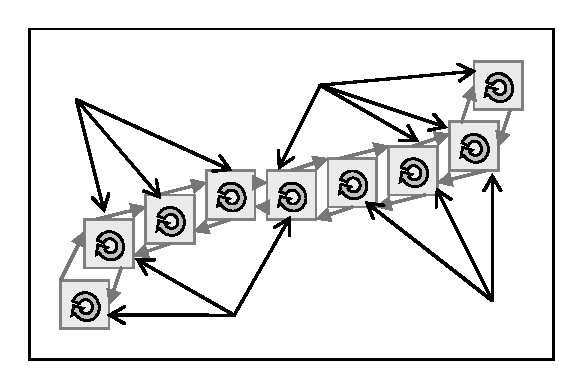
\includegraphics[scale=0.75]{Tissues/tissues-antigen}
	\caption{Multiple tissue model and the situated spatial properties that may affect antigenic exposure.}
	\label{fig:tissues:exposures:model}
\end{figure}

\begin{figure}[ht]
	\subfloat[Example Symmetric Tissue Exposure.]{
	\label{fig:tissues:examples:exposures:symmetric} %% label for first subfigure
	\begin{minipage}[c]{0.5\textwidth}
		\centering 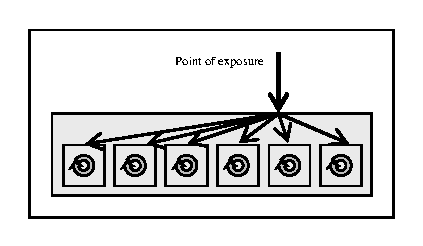
\includegraphics[scale=0.90]{Tissues/tissues-antigen-exposures-all}
	\end{minipage}}%
	\hfill
	\subfloat[Example Asymmetric Tissue Exposure.]{
	\label{fig:tissues:examples:exposures:asymmetric} %% label for second subfigure
	\begin{minipage}[c]{0.5\textwidth}
		\centering 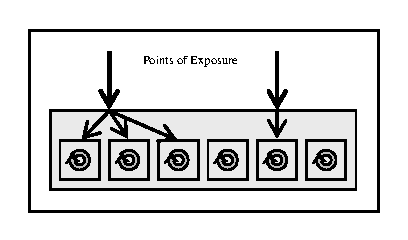
\includegraphics[scale=0.90]{Tissues/tissues-antigen-exposures-selective}
	\end{minipage}}
	\caption{Example of two different Tissue Exposure Regime with controlled selection of discrete repertoires on exposure events.}
	\label{fig:tissues:exposures:examples} %% label for entire figure
\end{figure}

% infection as a metaphor for what this is all about
In order to provide symmetry in the problem domain with the raise in the level of abstraction in the system, a new abstraction of the antigenic exposure paradigm is required. The exposure paradigm at the cellular level was concerned with an antigen of determinants, thus a suitable metaphor for an exposure of a tissue is an \emph{Infection of Antigen}. An infection is defined as the invasion and multiplication of a pathogenic micro-organism that may cause injury the the tissues. This definition provides a suitable metaphor for the point-wise exposure of tissue for two reasons (1) invasion and replication suggests a single antigenic type (pattern) perhaps with variation, and (2) tissue injury promotes urgency which may be interpreted as efficient and effective response, whether it is acquired in the tissue or imported from surrounding tissues. Although the abstraction is pathogen-centric given both the exogenous origin and selected metaphor, one may just as easily use a endogenous-centric metaphor such as tumour occurrence and growth. In both cases the abstraction properties of discrete (point-wise) information mediation hold.

%
% Spatial-Temporal Exposures
%
\subsubsection{Spatial-Temporal Exposures}
\label{subsec:tissues:paradigm:exposures:spatialtemporal}
The specifics of the Tissue Exposure Regime may or may not be in the control of tissue model, which is dependant on the application domain and model configuration. One may consider a possibility space of all exposure-to-repertoire interactions and consider questions of lymphocyte movement types in the context of desirable system behaviours under different regimes. Irrespective of the exposure properties, the concern of the system is to address \emph{what repertoires} are exposed at \emph{what times}. These concerns may be generalised to that of spatial and temporal consistency of exposure patterns. \emph{Temporal consistency} refers to the systems anticipation of the amount of memory required. \emph{Spatial consistency} refers to systems anticipation and the positioning of lymphocytes across the repertoires. A lack of consistency in either dimension removes the ability of a system to anticipate specifically, requiring general (all-repertoire, all-time) anticipation. It is important to highlight that the temporal memory applies system-wide without spatial memory (in the face of spatial inconsistency), and spatial memory applies for all time without temporal memory (in the face of temporal inconsistency). Therefore, the default case is remember everything everywhere for all time in the face of spatial and temporal inconsistency. This is an important implication of the antigenic exposure paradigm as it defines the role of inter-repertoire cell movement as the exploitation of patterns in the combination of spatial and temporal consistency of system exposures such that the response memory may be generated and shifted (adapted) in response to changes in the spatial or temporal properties of the exposure. 

% memory
The \emph{Temporal Memory Effect} refers to the systems capability to retain an impression of an exposure event and recall that impression to provide an improved (compared to random) response under similar circumstances in the future. The effect is intuitive for a single repertoire model where it may be facilitated by memory cells or a change in cell compositional densities. The exploitation of the cells becomes a probabilistic function of the antigen encountering a memory in the repertoire. Figure~\ref{fig:tissues:effects:temporalmemory} provides a depiction of the temporal memory effect in a single repertoire, where cell attrition via repertoire `turn over' results in the fading of acquired information over time.

\begin{figure}[ht]
	\centering
	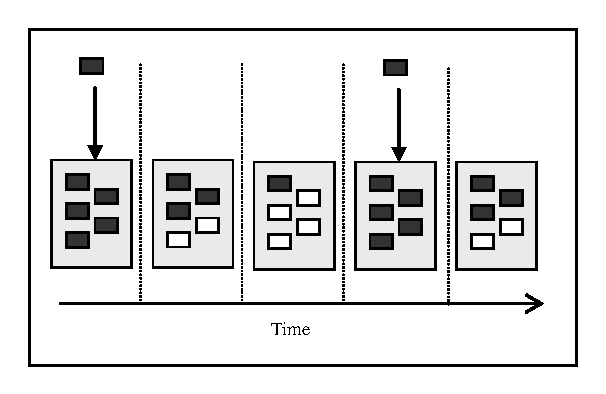
\includegraphics[scale=0.75]{Tissues/tissues-effects-temporalmemory}
	\caption{Depiction of the temporal memory effect in a single repertoire model over time, where the arrows at the top represent information flow into the system and the arrow along the bottom represents time.}
	\label{fig:tissues:effects:temporalmemory}
\end{figure}

The multiple repertoire model further requires the dissemination of memory across multiple repertoires. The memory represents a system-wide spatial anticipation of future exposures to the same or similar antigen. The following summarise the properties of temporal memory in the single repertoire model:

\begin{itemize}
	\item \emph{Short Term}: A response results in a large short-term memory in the form of effector cells (short lifespan), which are useful initially at the point of exposure, and disseminated throughout the system.
	\item \emph{Long Term}: A response results in a small long-term memory in the form of memory cells (long lifespan), which also disseminate throughout the system.
	\item \emph{Memory Size}: The larger the antigen dose, the larger the short-term and long-term memories.
	\item \emph{Memory Stability}: With the increases in the frequency of exposures (over the systems lifetime), the larger and more stable the long-term memory. The memory size is expected to reach a point of stability where antigen-to-memory cell match is practically assured.
\end{itemize}

This \emph{Spatial Self-Organisation Effect} is an emergent property of point-wise exposure of repertoires in the face of lymphocyte recirculation. The exposure and stimulation of a repertoire results in a response to the pathogen. The exposure is spatial, therefore the response is spatial. The following summarises the properties of spatial self-organisation in the discrete repertoire model:

\begin{itemize}
	\item \emph{Interaction}: (response maturation) The clonal selection principle raises a maturated response to the antigen that results in effectors and memory cells. Some of the raised clone disseminates early, although the majority remains during the stimulation of the repertoire. This is the formation of a germinal centre and constraints are imposed on outbound lymphocytes.
	\item \emph{Recruitment}: (response amplification) The repertoire tissue becomes inflamed resulting in the increased intake of recirculating lymphocytes, a response amplification effect via lymphocyte sequestration. The inbound cells may be \naive\ cells, effector cells, or memory cells and may or may not have improved specificity for the pathogen than the cells already in the repertoire.
	\item \emph{Homing}: (preferential recirculation) Memory cells created in a specific repertoire, preferentially recirculate back to that repertoire, in an effort of spatial anticipation of the same antigen in the same place.
\end{itemize}

\begin{figure}[ht]
	\centering
	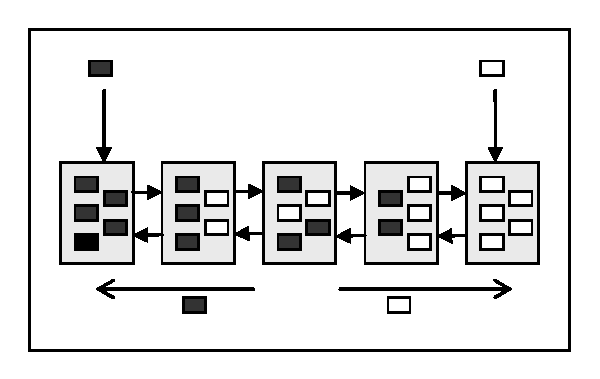
\includegraphics[scale=0.75]{Tissues/tissues-effects-spatialorganisation}
	\caption{Depiction of the repertoire specialisation that results in the Spatial Self-Organisation effect, where the arrows from above represent information flow into the system and the arrows below represent dissipation of acquired information.}
	\label{fig:tissues:effects:selforganisation}
\end{figure}

The result of the general behaviours of the tissues and the cells is a specific spatial response strategy that attempts to get the best from the system at the point of exposure in a bottom-up manner. The spatial organisation may extend through time, such that in addition to the patrolling effectors and memory cells that disseminate throughout the system, effectors may remain behind and provide a short-term memory and spatial anticipation of response. The following summarises the effects of spatial self-organisation in the discrete repertoire model:

\begin{itemize}
	\item \emph{Localisation}: Specific response at the time and the location of the exposure. Natural spatial-temporal response.
	\item \emph{Surveillance}: Long-term and short-term memory in recirculation anticipating the exposure system wide. The premise that the system may be exposed to the same pathogen again the future.
	\item \emph{Sentinels}: Short-term memory, stationary at the point of exposure, anticipating exposure at the same location. The premise that a location that has been exposed may be exposed again.
\end{itemize}

Spatial anticipation is facilitated in the short-term by sentinel effectors and in the long-term by memory cell homing patterns. In addition to the spatial self-organisation effect, the system mixes (perhaps disorganisation) the acquired immunity across the repertoires of the system. The principles of spatially mixing response effectors and memory provide a system-wide uniform (or consistent) response to a previously encountered pathogen. This ensures that immunity learned at one exposure point of the system, may be exploited elsewhere (anywhere) in the system.

\begin{figure}[ht]
	\centering
	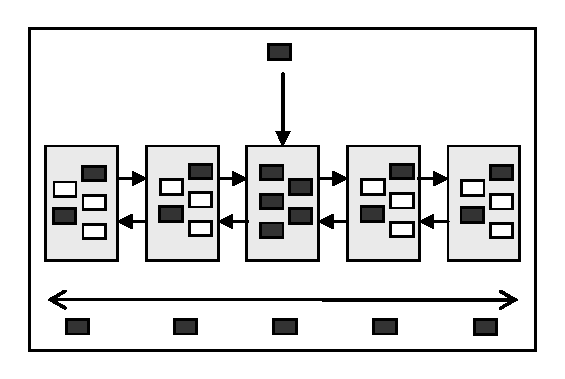
\includegraphics[scale=0.75]{Tissues/tissues-effects-consistent}
	\caption{Depiction of the unbiased dissemination of information that results in the Spatial Consistency of Response, where the arrow above represents information flow into the system and the arrow below represents information availability throughout the system.}
	\label{fig:tissues:effects:consistent}
\end{figure}

This effect called the \emph{Spatial Consistency of Response} is achieved through the information dispersal properties of lymphocyte recirculation that ensure that a fraction of the larger lymphocyte pool is in motion between the repertoires (immunosurveillance). The effect promotes system-anticipation rather than the more specific spatial-anticipation, and provides a distributed knowledge or memory that may rapidly self-organise to varied repertoire exposure patterns. The consistency provided is not strictly uniform, rather it is quasi-uniform, driven by the bottom-up stochastic decision properties that govern lymphocyte recirculation. From a lymphocyte perspective, movement in the face of unknown exposure patterns provides the system-wide goal of \emph{antigen-selection maximisation}. That is, lymphocytes exist to be selected by antigen, thus the behaviours of movement between, and residence within repertories seeks to maximise the change of this event occurring. As already described, this is already facilitated by the homing behaviour of memory lymphocytes, and the patrolling recirculation behaviour of effectors and \naive\ lymphocytes. Some concerns of this behaviour are (1) the quantity of the immunity acquisition, and (2) the rate of dispersal of the memory. The following summarises the concerns with achieving consistency of response:

\begin{itemize}
	\item \emph{Acquisition Quantity}: The system response may be proportional to the exposure, although the memory (both short-term and long-term) must be sufficient to provide coverage to all repertoires of the system. This memory is additive, and is expected to expand in proportion to additional exposures by the same pathogen. 
	\item \emph{Acquisition Dispersal}: The memory of an exposure originates at the point of exposure, and the delay of dispersal is a function of the (1) quantity of the memory, (2) the size (number of repertoires) and connectivity of the system, and (3) the rate of recirculation. Dispersal of acquired immunity must be such that coverage (probabilistic) of all repertoires is obtained within a reasonable amount of time.
\end{itemize}

The dispersal or mixing effect in the consistency of response facilitates the blind (recirculation) and specific (recruitment) sharing of acquired immunity between repertoires. Sharing may refer to the exploitation of specific immunity at a exposure location different from that at which it was acquired. Further, sharing may also refer to the cross-reactive effects achieved through less specific acquired immunity. This effect includes the ability of the system to generalise from varied exposure types such that new variations and combinations may also be exploited.

\begin{figure}[ht]
	\centering
	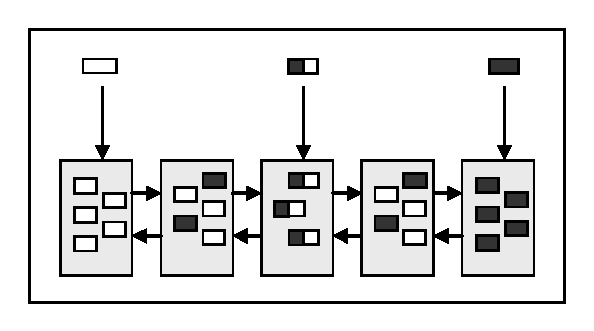
\includegraphics[scale=0.75]{Tissues/tissues-effects-sharing}
	\caption{Depiction of information sharing and a cross-reactive response, where the arrows above represent the flow of information into the system as well as an implicit anticipation for the application of acquired information.}
	\label{fig:tissues:effects:sharing}
\end{figure}

The integration of these features is a system that is expected to be plastic in its response capability, although is still capable of generating, maintaining, and self-organising a specific response to external stimulation. This behaviour may represent a trade-off in efficiency and efficacy of response between (1) system-wide consistency of response, and (2) segregation of response into specialised spatial compartments. The system may be configured to achieve one or the other of these effects, although achieving both effectively and concurrently represents the challenge for the system in unknown environments.

\begin{figure}[ht]
	\centering
	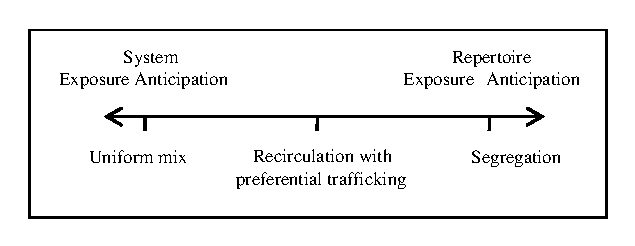
\includegraphics[scale=0.75]{Tissues/tissues-effects-integration}
	\caption{Depiction of the trade-off between the general anticipation of exposure and organised anticipation of exposure.}
	\label{fig:tissues:effects:integration}
\end{figure}


%
% Architectures
% Based on: Information Processing with a Lymphoid Tissue Architecture
%
\subsection{Tissue Architectures}
\label{subsec:tissues:paradigm:architectures}
%
% Exploiting Tissue Responsibilities
%
\subsubsection{Exploiting Tissue Responsibilities}
This section describes a lymphoid tissue model in which the tissue types (nodes) constrain the cell-based information processing that may occur to the cells housed within. Tissues are considered the units of adaptation that may receive and transmit information. Cells are the substrate for tissues knowledge representation, communication, and adaptation. This section describes a number of tissue-tissue interactions. 

%
% Cell Formation
%
\paragraph{Cell Formation}
\Naive\ lymphocytes are created in primarily lymphoid tissue. A \naive\ lymphocyte is generated in a pseudo-random manner. It represents an untested guess of a unit of information that may be useful to the system. A \naive\ cell may be created in one primarily lymphoid tissue and migrate to another for specialisation, similar to the migration of pre-lymphocyte cells from the bone marrow to the thymus to become \naive\ T-cells. Those cells that remain in the bone marrow become B-cells. The primary tissue nodes may condition the formed \naive\ cells. For example, the cells may be subjected to a negative and positive selection process such as that subjected to T-cells in the thymus. The result of such a process is the assessment and ultimate judgement of the feasibility of the proposed information guesses that the cells represent. In addition to the migration of \naive\ cells between primary lymphoid tissue for maturation, \naive\ cells may uni-directionally migrate from primary to secondary lymphoid tissue. This represents an upgrade in status for the cell from unprepared to prepared \naive\ cells, ready for information processing in the secondary tissue. As an interaction between primary and secondary lymphoid tissue it represents a transmission of feasible quasi-random information that may be useful to the system.

\begin{figure}[ht]
	\centering
	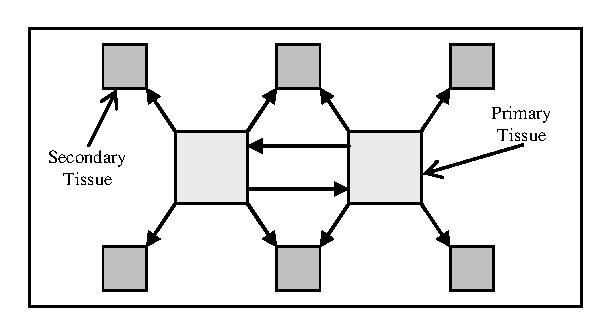
\includegraphics[scale=0.75]{Tissues/tissues-architectures-formation}
	\caption{Depiction of the relationship between primary and secondary lymphoid tissues, where the arrows show the sharing of information between primary tissues and the outward push of information from primary to secondary tissues..}
	\label{fig:tissues:architecture:formation}
\end{figure}

%
% Cell Maturation
%
\paragraph{Cell Maturation}
Secondary tissues houses many \naive\ lymphocytes as well as some memory cells and effectors if available. The tissue accepts a steady stream of \naive\ lymphocytes from primary tissue and integrates them into the cell population. Secondary tissue is responsible for exposing resident cells to antigen and facilitating any immune response that occurs as a result. Exposure is selection of cognate receptors for a given antigen, and response is the clonal selection process or similar as outlined in previous models. The result of the response are memory cells which have demonstrated their usefulness, and effector cells for addressing the immediate concerns of the antigen. Effector cells may or may not be given an impression of the tissue origin of the antigen (site of infection), as considered in the case of T-cell homing. Memory cells and non-homing effector cells recirculate between secondary tissues (lymph nodes for example), using the vascular system as the transport mechanism. The recirculation of memory and effector cells between secondary lymphoid tissue represents a transmission of acquired information regarding the environment. Portions of acquired information (individual cells) are shared between secondary tissues such that the information may be available for application or further maturation. Acquired information in the form of effector cells is transmitted from the location of maturation in the secondary tissue, to the location of application in the tertiary tissue.

\begin{figure}[ht]
	\centering
	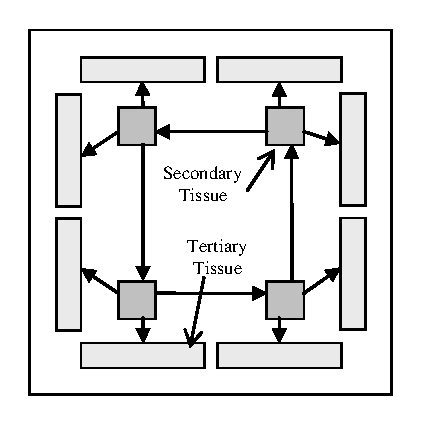
\includegraphics[scale=0.75]{Tissues/tissues-architecture-maturation}
	\caption{Depiction of the relationship between secondary tissues and secondary and tertiary tissues, where the arrows show the sharing of information between secondary tissues and the outward push of information from secondary to tertiary tissues.}
	\label{pic:tissues:architecture:maturation}
\end{figure}

%
% Cell Application
%
\paragraph{Cell Application}
Tertiary tissues accept and house many effector cells. The tissues accept a steady stream of effectors from locally connected secondary tissues, which are integrated into the population. Tertiary tissues are responsible for being receptive to pathogenic infection, thus may be considered receptive fields for information from the environment. The effector cells are employed at the sites of infection as needed, addressing the major function of their life cycle: application. Samples of the antigen may be taken from the site of infection in the tertiary tissue and transported into secondary tissue by courier cells, taking in addition information as to where the antigen was collected (to facilitate homing). Samples of antigen and some effector cells may be drained back into locally connected secondary tissue. This draining effect is facilitated by the lymph fluid that permeates tertiary tissues. The secondary tissue collections and filters the lymph for antigen, which are presented to resident lymphocytes. Pathogen exposure to tertiary tissue represent samples of the environment collected by the system. Different tertiary tissues may collect samples in different ways (for example skin, food, respiratory). The couriering and streaming of samples of pathogen back to secondary tissue provides a transmission of sensory information from the environment to areas of the system that can be adapted to address it. 

\begin{figure}[ht]
	\centering
	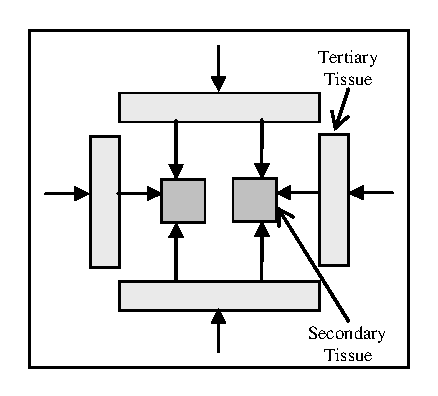
\includegraphics[scale=0.75]{Tissues/tissues-architecture-application}
	\caption{Depiction of the relationship between tertiary and secondary tissues and tertiary tissues and the environment, where the arrows depict the flow of information from the environment to the tertiary tissues and ultimately to the secondary tissues.}
	\label{fig:tissues:architecture:application}
\end{figure}

%
% Integration
%
\subsubsection{Integration}
The aggregation of all three tissue types describes an integrated model with layered information processing. From the inside out, the information availability increases in maturation (usefulness). The tertiary tissue contains no other cells than those known to be immediately useful, the primary tissue contains no other cells than those whose usefulness is unknown. The secondary tissues act as the mediator between these two extremes, providing the testing and maturation processes for information acquisition. The outward flow of prior knowledge through the layers of the system, whereas information about the environment flows inward. Principle pathogen exposures occur in the tertiary tissue where it may be addressed by resident effectors. If sufficiently large or novel, samples of the pathogen find their way into secondary tissue (courier or stream) for presentation to the learning mechanisms of the system. Therefore, lymphocytes migrate from the centre of the system outward, increasing in proficiency as they approach the surface, whereas pathogen are housed in the outer layer and seep into the second tier.

\begin{figure}[ht]
	\centering
		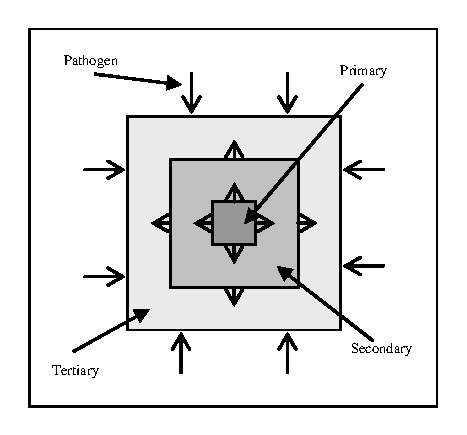
\includegraphics[scale=0.75]{Tissues/tissues-models-flows}
	\caption{Depiction of the layered tissue architecture and information flows between the layers, the arrows show the flow of information from the environment into the system as well as the outward push of new detectors from the centre of the system.}
	\label{fig:tissues:architecture:flows}
\end{figure}

Antigens that penetrate the system and manage to take-up residence in the tertiary tissue are drawn to the lymph nodes of the secondary tissue by fluid called lymph. Lymph drains into the lymph nodes, which in turn filter the fluid collecting antigens, which are presented to local and recirculating lymphocytes. From an information processing perspective, a lymph node is provided an information stream from the regionally located tertiary tissue. A proportionally large region of tertiary tissue feeds pathogen to a single lymph node, in effect proving multiple feeding information channels. The information is collected is specialised regions within the node. B-cells are exposed to the presented information, and if sufficiently activated may migrate to another specialised region on the node and form a germinal centre in which bouts of selection, proliferation, receptor maturation and ultimately cell differentiation occur. The product of this learning process are effector cells called plasma cells that produce antibodies for the triggering antigen in large numbers, and mature long-lived memory cells. The antibodies enter the blood stream and seek a serendipitous interaction with their cognate antigen. The memory cells recirculate between the secondary tissue and sometimes move into the tertiary lymphoid tissue, with the same mission. There is no homing effect for the B-cells. Their effectors flood the system, and their memory cells patrol. Importantly, the effectors and the memory cells are created and released in the vicinity of where the pathogen was encountered. Thus, they are more likely to encounter their cognate antigen sooner rather than later. 

\begin{figure}[ht]
	\centering
		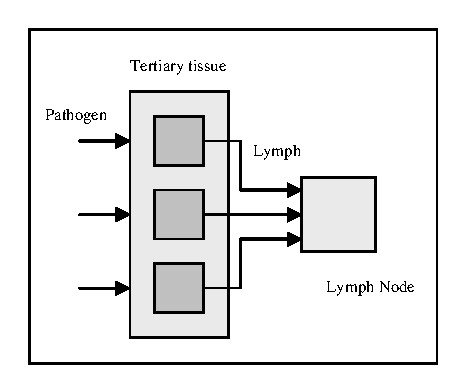
\includegraphics[scale=0.75]{Tissues/tissues-models-streaming}
	\caption{Depiction of the information streaming providing by lymph collecting in lymph nodes.}
	\label{fig:tissues:architecture:streaming}
\end{figure}

Another type of cell, called a dendritic cells, patrol tertiary tissue for pathogen. Once detected, these cells collect the material and migrate into the secondary lymphoid tissue (such as lymph nodes). In the secondary tissue, the dendritic cells present the pathogenic material to T-cells that respond, proliferate, and differentiate. The product of this learning process is mature T-cells in the form of effectors and likely long-lived memory cells. The effector T-cells are imprinted by the dendritic cell as to the location in the tertiary tissue of the pathogen exposure. The effectors recirculate the system and penetrate the tertiary tissue when the specific chemical signature is detected. Information is streamed from the tertiary tissue to the secondary tissue although the streaming is facilitated by courier cells. These cells are aware of where they collected their material and thus are capable of imprinting that information onto the produced effector cells. The result is an effect that differentiates the lymphocyte movement behaviour from that of the B-cells (that blindly seek their cognate antigen), to the T-cells (that home into the chemical signature of infected tissue).

\begin{figure}[ht]
	\centering
		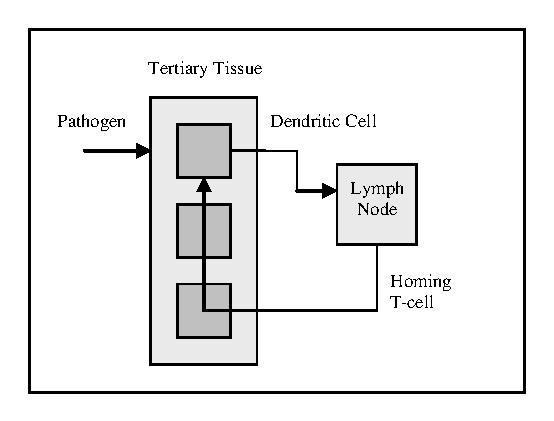
\includegraphics[scale=0.75]{Tissues/tissues-model-courier}
	\caption{Depiction of the courier-like behaviour of dendritic cell's.}
	\label{fig:tissues:architecture:courier}
\end{figure}

%
% Tissue Models
%
\subsubsection{Tissue Modes}
The information properties of the system have been described with regard to the transmission of the information substrate (immune cells) between the layers and within the layers. Table~\ref{tab:tissue:architectures:algorithms} lists the abstracted immunological functional behaviour required to meet the information processing needs outlined for the architecture.

\begin{table}[ht]
	\centering\small
		\begin{tabular}{lll}
		\toprule
		\textbf{Tier} & \textbf{Information Processing} & Behaviour \\ 
		\toprule
		1 & Generation and feasibility testing & Negative Selection \\ 
		2 & Maturation & Clonal Selection \\ 
		2 & Homoeostasis & Elaborated Clonal Selection \\ 
		2 & Recirculation & Recirculation Algorithm \\ 
		2-3 & Courier/Homing & Homing Algorithm \\ 
		2-3 & Exposures/Streaming & Antigenic Exposure \\ 
		2-3 & Inflammation & Recruitment Algorithm \\ 
		\bottomrule
		\end{tabular}	
	\caption{Summary of information processing needs, and proposed algorithms that meet those needs.}
	\label{tab:tissue:architectures:algorithms}
\end{table}

The information processing constraints of each tissue type, outline a clear responsibility for each tier of the architecture. Primary tissue is concerned with information generation and the pre-processing of information before it is employed in a learning process. Secondary tissue is responsible for learning, for identifying which internal information is presently useful and attempting to improve it (maturation), whilst at the same time applying it (effectors). The second tier is also responsible for the generation and maintenance of longer term memory, and the selective application of acquired memory. The tertiary tissue is responsible for providing an interface to the environment, mediating the application of acquired knowledge to sensory signals, with the filtering of temporally novel signals to secondary tissues for response generation.

\begin{table}[ht]
	\centering\small
		\begin{tabular}{ll}
		\toprule
		\textbf{Tissue Type} & \textbf{Responsibility} \\ 
		\toprule
		\emph{Primary Tissue} & Information generation (preparation) \\ 
		\emph{Secondary Tissue} & Information maturation (learning and memory) \\ 
		\emph{Tertiary Tissue} & Information application (sensory) \\ 
		\bottomrule
		\end{tabular}	
	\caption{Summary of the principle responsibility of each tier of the architecture.}
	\label{tab:tissue:architectures:tiers}
\end{table}

The majority of the clonal selection information processing occurs in the secondary lymphoid tissue. The other two layers may be easily incorporated into the secondary tissue, providing only conceptual attributes of the tissue model. This compression of responsibility has been implicit in previously proposed clonal selection, negative selection, and other cell-theory based algorithms. Given that the tissues may be compressed, it is important to consider the utility of separating the proposed responsibilities into a dependant hierarchy of layers.

\begin{figure}[ht]
	\centering
	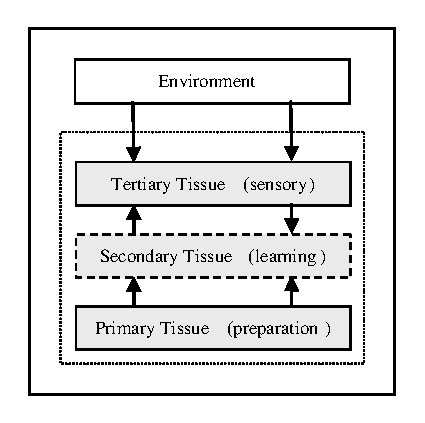
\includegraphics[scale=0.75]{Tissues/tissues-architecture-integration}
	\caption{Depiction of the layered information processing properties of the lymphoid tissue architecture.}
	\label{pic:tissues:architecture:layered}
\end{figure}

This section proposes three different models that employ the proposed lymphoid tissue architecture. Each model is inspired by a different aspect of the acquired immune system, from a lymphatic system (tissue) perspective. The principles for separated responsibility are (1) the centralised generation of \naive\ cells facilitating centralised prior knowledge, (2) consolidated secondary tissue for a networked learning architecture large enough to meet the needs of the system, (3) a large host consisting predominantly of tertiary tissue, which provides a distributed sensor platform for receiving and responding to environmental signals.

%
% Filter Model
%
\subsubsection{Filter Model}
The filter model is inspired by the specialisation of the lymphatic system at the primary entry points for exogenous antigen (pathogen). Examples include the tonsils and related tissues for addressing pathogen that enter the host via the respiratory system, the Peyer's patch tissues in the intestines that addressing pathogen that enter the host via the digestive system, and the spleen that filters the blood for pathogen. The model contains a single point of entry for pathogen (tertiary tissue), which is monitored by one or a small collection of secondary lymphoid tissues. The secondary tissue is supported by a single source of \naive\ cells (primary tissue).

\begin{figure}[ht]
	\centering
	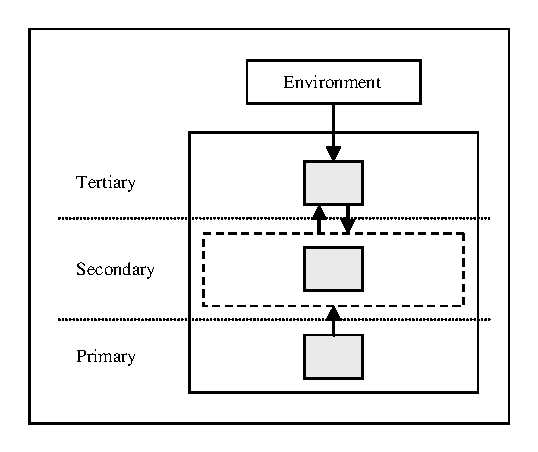
\includegraphics[scale=0.75]{Tissues/tissues-models-filter}
	\caption{Depiction of the simple filter model.}
	\label{pic:tissues:architecture:filter}
\end{figure}

Although the model is called a \emph{filter} (the basis for its inspiration) it is not restricted to filtering information processing tasks. The focus of this model is on the system possessing a single point of entry for pathogen (sensory signals) although at a high load (many signals), and one or a small number of specialised secondary tissues to address the needs of the tertiary tissue. 

\begin{table}[ht]
	\centering\small
		\begin{tabular}{ll}
		\toprule
		\textbf{Tissue Type} & \textbf{Configuration} \\ 
		\toprule
		\emph{Primary} & Single tissue feeding the secondary tissue. \\ 
		\emph{Secondary} & Single (or a small number) secondary tissues with high capacity of cells. \\ 
		\emph{Tertiary} & Single point of entry for the system to monitor. \\ 
		\bottomrule
		\end{tabular}	
	\caption{Configuration of the architecture for the filter model.}
	\label{tab:tissue:architectures:filter}
\end{table}

%
% Lymph Node Model
%
\subsubsection{Lymph Node Model}
The lymph node model is inspired by the network of lymph nodes, connected by the vascular system, that receive antigen as a stream in the lymph. The model is more complex than the filter model as it contains a network of moderately sized secondary lymphoid tissues that recirculate memory and effector cells. Further, unlike the filter model, it has a large receptive field of tertiary tissue, which provides a single broad sensory system.

\begin{figure}[ht]
	\centering
	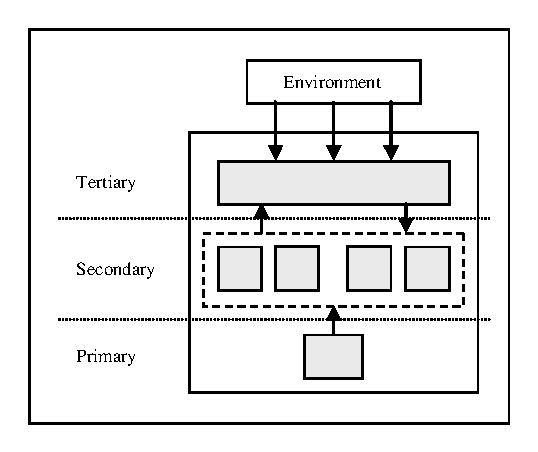
\includegraphics[scale=0.75]{Tissues/tissues-models-lymphnode}
	\caption{Depiction of the lymph node model.}
	\label{pic:tissues:architecture:lymphnode}
\end{figure}

The focus in this model is the large tertiary tissue receptive field, and the network of secondary tissues (lymph nodes), in particular the capabilities of the lymph nodes to recirculate mature cells (share acquired information), and their capabilities in trafficking effectors into tertiary tissues (applying acquired information).

\begin{table}[ht]
	\centering\small
		\begin{tabularx}{\textwidth}{lX}
		\toprule
		\textbf{Tissue Type} & \textbf{Configuration} \\ 
		\toprule
		\emph{Primary} & Single tissue feeding the secondary tissue. \\ 
		\emph{Secondary} & A consolidated network of moderate sized secondary tissues.  \\ 
		\emph{Tertiary} & A large and uniform receptive field for input signals.  \\ 
		\bottomrule
		\end{tabularx}		
	\caption{Configuration of the architecture for the lymph node model.}
	\label{tab:tissue:architectures:lymphnode}
\end{table}

%
% Host Model
%
\subsubsection{Host Model}
The host model is an integration of one or more filter models with the lymph node model. The resultant model is a larger-scale tissue architecture that may be equated to a lymphatic system of a host. The model is composed of a variety of different tertiary tissue types and thus different meanings for the secondary tissue to be provided with antigen to present to resident cells. In addition, the secondary tissue is made of a core network of lymph nodes, as well as collections of specialised lymphoid tissue to address principle pathogen penetration areas. Finally, the system has one or more primary lymphoid tissues for the creation and dissemination of \naive\ cells to secondary tissues.

\begin{figure}[ht]
	\centering
	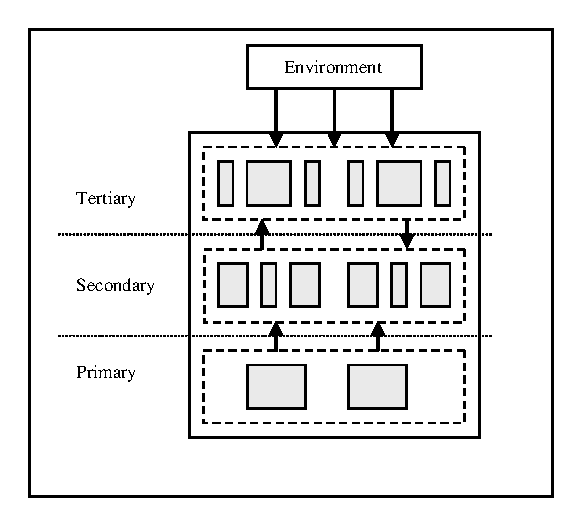
\includegraphics[scale=0.75]{Tissues/tissues-models-host}
	\caption{Depiction of the host model.}
	\label{pic:tissues:architecture:host}
\end{figure}

The focus of the model is the integration of the lymph node network (and related method for sampling antigen from tertiary tissue) with a number of filter-based models centred around primary pathogen access points. This host model represents a hybrid integration of the two sub-types of tissue architectures, and culminating (pinnacle in complexity) lymphatic tissue model.

\begin{table}[ht]
	\centering\small
		\begin{tabularx}{\textwidth}{lX}
		\toprule
		\textbf{Tissue Type} & \textbf{Configuration} \\
		\toprule
		\emph{Primary} & Set of primary tissues feeding the secondary tissue. \\
		\emph{Secondary} & A backbone of a consolidated network as well as specialised regions for each major entry point (diverse.  \\
		\emph{Tertiary} & Multiple tertiary tissues of varied size and scope (diverse)  \\
		\bottomrule
		\end{tabularx}		
	\caption{Configuration of the architecture for the host model}
	\label{tab:tissue:architectures:host}
\end{table}

%
% Summary
%
\subsubsection{Summary}
The lymphoid tissue components, exposures, and architecture models provide a context for the previously defined adaptive models of the Cellular Paradigm concerning immune cells (\emph{intra-tissue}), and a context for novel cell migration adaptive models to be investigated (\emph{inter-tissue}). The applications of the architecture in the proposed lymphoid tissue models provides three specific settings for integrated lymphoid tissue-based information processing. This section suggested at the potential for Tissue Clonal Selection and more generally tissue-based Artificial Immune System algorithms, as a scale above the state of classical cell-based Artificial Immune System algorithms.

%
% Realised Tissue Paradigm
%
\section{Realised Tissue Paradigm}
\label{subsec:tissues:paradigm:method}
% viability of the paradigm
A single immune system of tissues that may be exposed to infections provides an effective metaphor for considering the problem of the acquisition of information in a decentralised manner from a distributed environment, and strategies toward the anticipated application of acquired information. The presentation of the lymphatic system demonstrated that some infections can be localised to predictable lymphoid tissues (peripheral immune system) and others cannot (systemic immune system). Therefore a host immune system of lymphoid tissues must simultaneously manage predicted, unpredicted, and a variety of intermediate antigenic infections from its antigenic habitat. Toward this end, the host immune system considers the differential mobility of cells between tissues and differential cell types as a strategy for managing so-called anticipated and unanticipated antigenic infections across all tissues. 
% this section
This section provides a realisation of the concerns of the abstract Tissue Clonal Selection Paradigm presented in Section~\ref{sec:tissues:paradigm}. This includes definitions of a tissue problem in the Infection Exposure Problem and specialisation in colour space, and the Tissue Clonal Selection Algorithm that provides a basis for investigation into cell trafficking schemes. A series of tissue-based measures are presented for assessing tissue algorithms on colour space realisations of infection problems that provide quantitative indicators regarding the concerns of spatial temporal exposures. Collectively, this section provides a basis for the implementation and exploratory empirical investigation into the Tissue Clonal Selection Paradigm, as well as a bridge between the the biology (Section~\ref{sec:tissues:migration}) and abstract models (Section~\ref{sec:tissues:paradigm}) of Tissue-centric Clonal Selection.

%
% Problem
%
\subsection{Antigenic Infections}
\label{subsec:tissues:paradigm:method:problems}
This section considers the realisation of the exposure paradigm outlined in Section~\ref{subsec:tissues:paradigm:exposures}. In particular, this section abstracts the Antigen Exposure Problem considered for the cellular paradigm for the tissue paradigm called an Infection, and specialises an instance of the problem in Colour Space. In addition, the discrete properties of tissue exposures are reconsidered and a number of specialised Tissue Exposure Regimes are defined.

%
% Infection Antigenic Exposure Problem (IAEP)
%
\subsubsection{Infection Antigenic Exposure Problem}
The Antigenic Exposure Problem (AEP) defined in Algorithm~\ref{alg:cells:realised:exposures:aep} provides a general problem definition where a Tissue $T$ is exposed to an Infection $I$. A given Cellular Clonal Selection Algorithm may be considered a single $T$ in a Host of Tissues ($H = \{T_1, T_2, T_3 \ldots, T_n\}$). Therefore the AEP must be generalised for interaction with an $H$. The \emph{Infection Antigenic Exposure Problem (IAEP)} defined in Algorithm~\ref{alg:tissues:problem:iaep} provides a generalised exposure problem in which an $H$ is exposed to a Habitat $B$ of Infections $I$ ($B = \{I_1, I_2, I_3, \ldots, I_n\}$).
% define the things used
The parameters $N_{determinants}$, $N_{antigen}$, and $N_{infections}$ define the properties of $B$ with a symmetrical number of $I$ which are passed to $CreateHabitat$ to create a problem instance. $Exposure$ refers to a given exposure mechanism, such as the variety of Tissue Exposure Regimes (TER) defined later in this section. An exposure regime returns a result set $H_{rs}$ that represents the state of a given $H$ with regard to its ability respond to the $B$ under the given TER.

\begin{algorithm}[ht]	
	\SetLine
	\SetKwData{Host}{H}
	\SetKwData{Habitat}{B}
	\SetKwFunction{StopCondition}{StopCondition}
	\SetKwFunction{CreateHabitat}{CreateHabitat}
	\SetKwFunction{Exposure}{Exposure}
	\KwIn{\Host, $N_{determinants}$, $N_{antigen}$, $N_{infections}$}
	\KwOut{$H_{rs}$}
	
  \Habitat $\leftarrow$ \CreateHabitat{$N_{determinants}$, $N_{antigen}$, $N_{infections}$}\;
  $H_{rs} \leftarrow$0\;
	\While{$\neg$\StopCondition{}}
	{
		$H_{rs} \leftarrow$ \Exposure{\Host, \Habitat}\;
	} 
	\Return{$H_{rs}$}\;
	
	\caption{Infection Antigenic Exposure Problem (IAEP).}
	\label{alg:tissues:problem:iaep}
\end{algorithm}

%
% Infection Colour Space Problem (ICSP)
%
\subsubsection{Infection Colour Space Problem}
% general ICSP
The IAEP may be specialised as an infection extension of the Antigen Colour Space Problem (ACSP) defined in Section~\ref{sec:cells:realised:exposures} called the \emph{Infection Colour Space Problem (ICSP)}. An instance of the ACSP involved the exposure of a $T$ to a set of Colour Space Patterns (CSP), where the goal of the problem is to minimise average error in the response $T_{rs}$. The ICSP specialisation of IAEP exposes a $H$ to a set of sets of CSP ($B$ of $I$'s), with the goal of minimising the average error in the response $H_{rs}$ (defined in Equation~\ref{eq:tissues:measure:he}).
% minimal case
One may define a minimal configuration of the IAEP and thus the ICSP that focus the concerns of the problem on the highest level of abstraction, the Habitat $B$. This focus is provided by reducing the configuration at levels below the desired level to minimal levels of complexity. A \emph{Minimal Infection Antigenic Exposure Problem (MIAEP)} is defined where $N_{infections}$ is variable, although $N_{antigen}$ and $N_{determinants}$ are fixed at 1. In the case of a minimal ICSP, the number of $I$ defines the number of CSP ($A$), each of which has a single $D$ comprised of all three Colour Space Components (Red, Green, and Blue).
% what does minimal give us, the focus

\begin{figure}[ht]
	\subfloat[General IAEP Configuration.]{
	\label{fig:tissues:exposures:general} %% label 
	\begin{minipage}[t]{0.50\textwidth}
		\centering 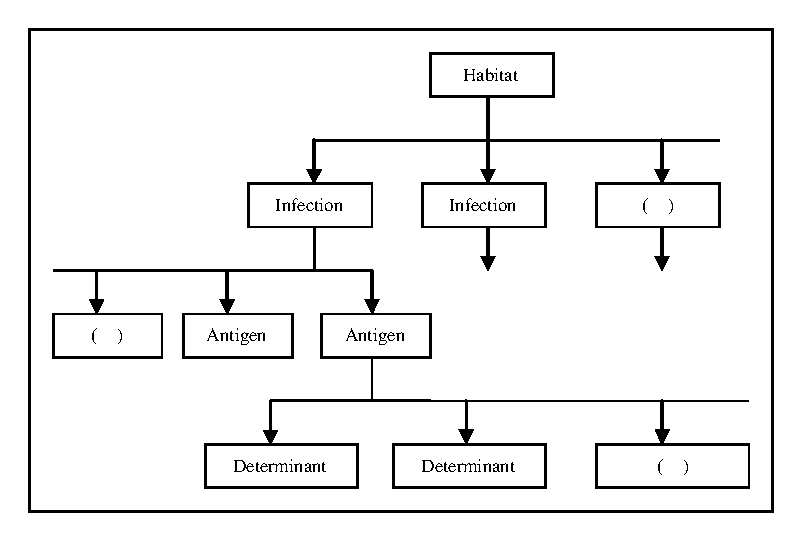
\includegraphics[scale=0.60]{Tissues/tissues-problem-case-general}
	\end{minipage}}%
	\hfill
	\subfloat[Minimal IAEP Configuration.]{
	\label{fig:tissues:exposures:minimal} %% label 
	\begin{minipage}[t]{0.50\textwidth}
		\centering 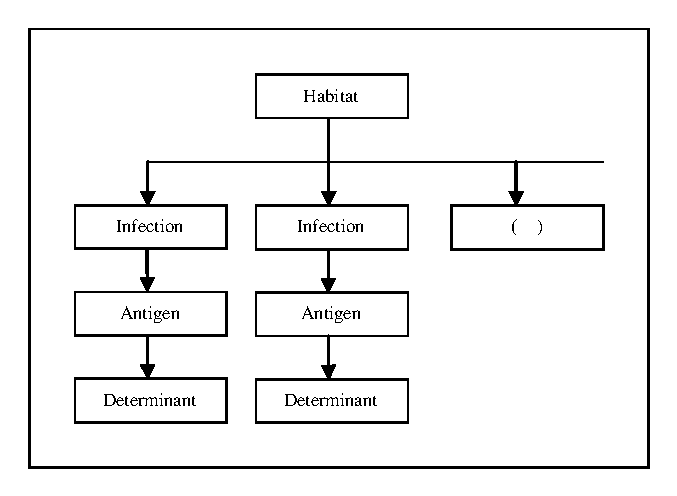
\includegraphics[scale=0.65]{Tissues/tissues-problem-case-minimal}
	\end{minipage}}	
	\caption{Depictions of general and minimal configuration examples of the Infection Antigenic Exposure Problem (IAEP).}
	\label{fig:tissues:exposures:problem} %% label for entire figure
\end{figure}

%
% Tissue Exposure Regimes
%
\subsubsection{Tissue Exposure Regimes}
% a reason varied tissue exposure patterns
Section~\ref{subsec:tissues:paradigm:exposures} defined the two important aspects of the problems that Tissue Clonal Selection Algorithms must address: (1) discrete tissue exposures, and (2) the spatial temporal properties of exposure anticipation defined by the regularity of a given tissue exposure regime. Toward this end, this section explicitly defines five different Tissue Exposure Regimes (TER) for specialising the $Exposure(H, B)$ of the IAEP providing examples from the range of possible regular and irregular exposures (spatial-temporal exposure of tissues) with some and all of the information in the problem domain. The schemes include: Symmetric Exposure, Asymmetric Exposure, Point Exposure, Random Exposure, and Probabilistic Exposure. The TER provides a mechanism by which to specialise an the infection exposures of a habitat to the tissues of a host, providing an generalisation of the limitations imposed by the structure, organisation, and properties of different tissues as described by the various tissue architectures in Section~\ref{subsec:tissues:paradigm:architectures}. Figure~\ref{fig:tissues:recirculation:exposures} provides a depiction of four of the five exposure regimes to a host of tissues.

\begin{figure}[ht]
	\subfloat[Symmetric Tissue Exposure Regime (STER).]{
	\label{fig:tissues:recirculation:exposures:symmetric} %% label 
	\begin{minipage}[t]{0.50\textwidth}
		\centering 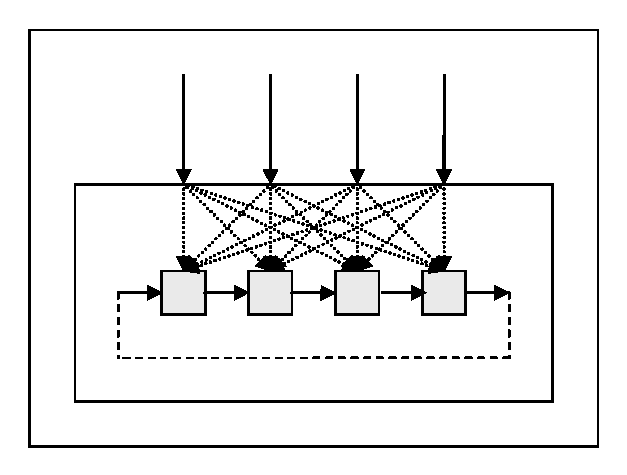
\includegraphics[scale=0.4]{Tissues/tissues-recirculation-exposure-symmetric}
	\end{minipage}}%
	\hfill
	\subfloat[Asymmetric Tissue Exposure Regime (ATER).]{
	\label{fig:tissues:recirculation:exposures:asymmetric} %% label 
	\begin{minipage}[t]{0.50\textwidth}
		\centering 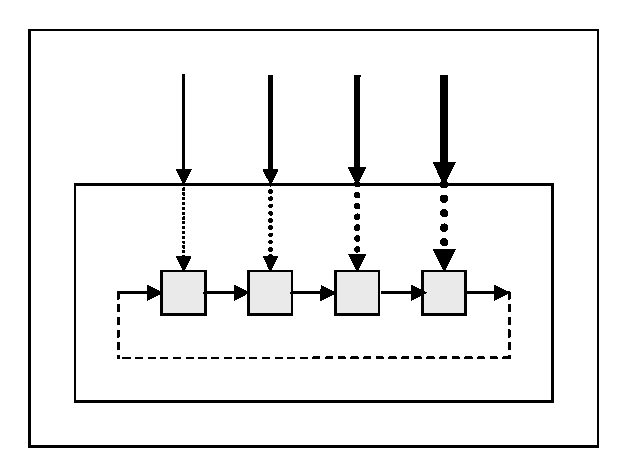
\includegraphics[scale=0.4]{Tissues/tissues-recirculation-exposure-asymmetric}
	\end{minipage}}\\
	% new line for second set
	\subfloat[Random Tissue Exposure Regime (RTER).]{
	\label{fig:tissues:recirculation:exposures:random} %% label 
	\begin{minipage}[t]{0.50\textwidth}
		\centering 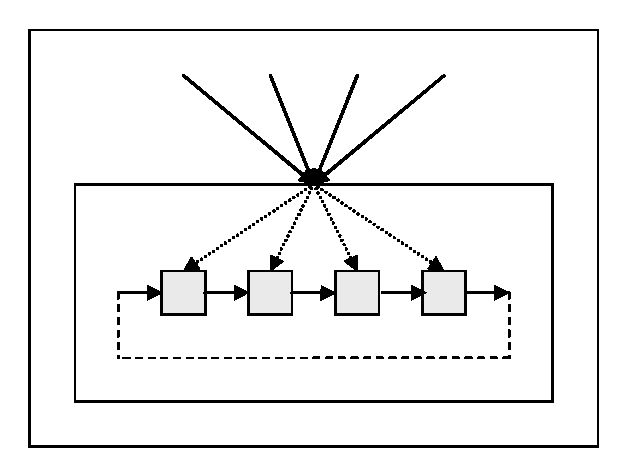
\includegraphics[scale=0.4]{Tissues/tissues-recirculation-exposure-random}
	\end{minipage}}%
	\hfill
	\subfloat[Point Tissue Exposure Regime (PTER).]{
	\label{fig:tissues:recirculation:exposures:point} %% label 
	\begin{minipage}[t]{0.50\textwidth}
		\centering 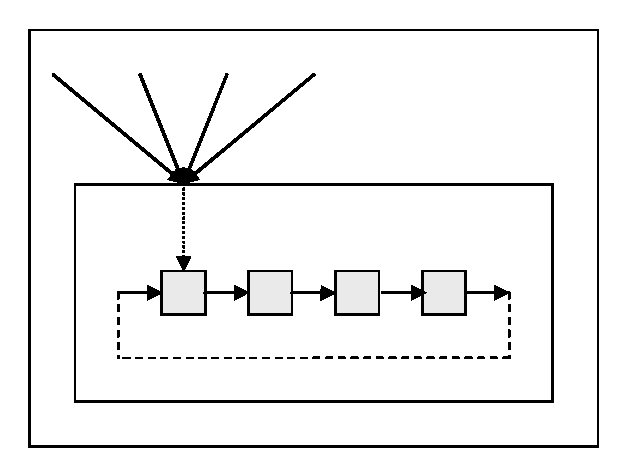
\includegraphics[scale=0.4]{Tissues/tissues-recirculation-exposure-point}
	\end{minipage}}%
	\caption{Depictions of the four different Tissue Exposure Regimes (TER).}
	\label{fig:tissues:recirculation:exposures} %% label for entire figure
\end{figure}

%
% Symmetric
%
\paragraph{Symmetric}
The \emph{Symmetric Tissue Exposure Regime (STER)} defined in Algorithm~\ref{alg:tissues:exposures:regime:symmetric} involves the exposure of each Infection $I$ to each Tissue $T$ (see Figure~\ref{fig:tissues:recirculation:exposures:symmetric}). Thus, each tissue is exposed to and must address the scope of the antigenic habitat $B$. 

\begin{algorithm}[ht]	
	\SetLine		
	\SetKwData{Host}{H}
	\SetKwData{Habitat}{B}
	\SetKwFunction{Exposure}{Exposure}
	
	\KwIn{\Host, \Habitat}
	
	\ForEach{$T_i \in$ \Host}	
	{
		\ForEach{$I_i \in$ \Habitat}
		{
			\Exposure{$I_i$, $T_i$}\;
		}
	}	
	\caption{Symmetric Tissue Exposure Regime (STER).}
	\label{alg:tissues:exposures:regime:symmetric}
\end{algorithm}

%
% Asymmetric
%
\paragraph{Asymmetric}
The \emph{Asymmetric Tissue Exposure Regime (ATER)} defined in Algorithm~\ref{alg:tissues:exposures:regime:asymmetric} involves the exposure of each $I$ Infection to a single Tissue $T$ in a consistent manner, such that once established the same $T$-to-$I$ mapping is used for each exposure (see Figure~\ref{fig:tissues:recirculation:exposures:asymmetric}). The number of $T$ may match the number of $I$ such that each $T$ addresses $\frac{1}{N_{infections}}$ per host exposure.

\begin{algorithm}[ht]	
	\SetLine		
	\SetKwData{Host}{H}
	\SetKwData{Habitat}{B}
	\SetKwFunction{Exposure}{Exposure}	
	\KwIn{\Host, \Habitat}
	
	\ForEach{$T_i \in$ \Host $\wedge I_i \in$ \Habitat}
	{
		\Exposure{$I_i$, $T_i$}\;
	}	
	\caption{Asymmetric Tissue Exposure Regime (ATER).}
	\label{alg:tissues:exposures:regime:asymmetric}
\end{algorithm}


%
% Point
%
\paragraph{Point}
The \emph{Point Tissue Exposure Regime (PTER)} defined in Algorithm~\ref{alg:tissues:exposures:regime:point} restricts the exposure of all $I$ to a single and consistent $T$ across all host exposures (see Figure~\ref{fig:tissues:recirculation:exposures:point}). The choice of $T$ that becomes the point of exposure for the host may be randomly selected from $H$.

\begin{algorithm}[ht]	
	\SetLine		
	\SetKwData{Host}{H}
	\SetKwData{Habitat}{B}
	\SetKwFunction{Exposure}{Exposure}	
	\KwIn{\Host, \Habitat, $T_{point}$}
	
	\ForEach{$I_i \in$ \Habitat}
	{
		\Exposure{$I_i$, $T_{point}$}\;
	}	
	\caption{Point Tissue Exposure Regime (PTER).}
	\label{alg:tissues:exposures:regime:point}
\end{algorithm}

%
% Random
%
\paragraph{Random}
The \emph{Random Tissue Exposure Regime (RTER)} defined in Algorithm~\ref{alg:tissues:exposures:regime:random} is similar to the asymmetric exposure regime, although the matching of $T$ with $I$ occurs randomly with re-selection each exposure (see Figure~\ref{fig:tissues:recirculation:exposures:random}). Thus, a given $T$ may be exposed to a different subset of the antigenic habitat $B$ each host exposure where it is possible for the set to be empty. 

\begin{algorithm}[ht]	
	\SetLine		
	\SetKwData{Host}{H}
	\SetKwData{Habitat}{B}
	\SetKwFunction{Exposure}{Exposure}	
	\SetKwFunction{RandomTissue}{RandomTissue}	
	\KwIn{\Host, \Habitat}	
	
	\ForEach{$I_i \in$ \Habitat}
	{
		$T_{point} \leftarrow$ \RandomTissue{$H$}\;
		\Exposure{$I_i$, $T_{point}$}\;
	}	
	\caption{Random Tissue Exposure Regime (RTER).}
	\label{alg:tissues:exposures:regime:random}
\end{algorithm}

%
% Probabilistic
%
\paragraph{Probabilistic}
The \emph{Probabilistic Tissue Exposure Regime (OTER)} defined in Algorithm~\ref{alg:tissues:exposures:regime:probabilistic} provides an intermediate specialisation of the RTER and ATER in which the selection of $T$ is probabilistic based on past selections providing probabilistic spatial consistency of re-exposure. In addition, the $I$-to-$T$ mapping is maintained for an extended number of host exposures before a probabilistic reselection is made, providing temporal regularity to the spatial exposures. The $duration$ parameter defines the number of host exposures (the $HostExposureNumber$ state variable) a selected $T$ is exposed to a given $I$. The state variable $Histogram$ keeps track of the frequency each $T$ is exposed to each $I$, and $biasedRouletteWheelSelection(Histogram)$ uses a biased roulette wheel selection routine on the histogram for a given $I$ over all $T$ to select a $T$ to expose for $duration$ host exposures. The $I_{tissues}$ state variable keeps track of which $T$ each $I$ has selected and should expose.

\begin{algorithm}[ht]	
	\SetLine		
	\SetKwData{Host}{H}
	\SetKwData{Habitat}{B}	
	\SetKwFunction{Exposure}{Exposure}
	\SetKwFunction{BiasedRouletteWheelSelection}{BiasedRouletteWheelSelection}
	\KwIn{\Host, \Habitat, $duration$, $Histogram$, $HostExposureNumber$, $I_{tissues}$}
	\ForEach{$I_i \in$ \Habitat}
	{
		% check if time to make a selection
		\If{($Epoch \bmod duration$) $\equiv$ 0}
		{
			% make a selection
			$T_i \leftarrow$ \BiasedRouletteWheelSelection{$Histogram_{I_i}$}\;
			% store selection
			${I_{tissues}}_i \leftarrow T_i$\;
			% remember the selection
			${Histogram_{I_i}}_{T_i} \leftarrow {Histogram_{I_i}}_{T_i} + 1$\;
		}
		\Exposure{$I_i$, ${I_{tissues}}_i$}\;
		$HostExposureNumber \leftarrow HostExposureNumber + 1$\;
	}	
	\caption{Probabilistic Tissue Exposure Regime (OTER).}
	\label{alg:tissues:exposures:regime:probabilistic}
\end{algorithm}

%
% Algorithms
%
\subsection{Tissue Clonal Selection}
\label{subsec:tissues:paradigm:method:algorithms}
% general algorithm
The Cellular Clonal Selection Algorithm (CCSA) defined in Algorithm~\ref{alg:cells:realisation:algorithms:ccsa:exposure} describes the general clonal selection interaction between an Infection $I$ and a Tissue $T$. The tissue paradigm requires a raise in the level of abstraction from a single $T$ to a Host $H$ of $T$ ($H = \{T_1, T_2, T_3, \ldots, T_n\}$) that responds to a Habitat $B$ of Infections $I$. \emph{Tissue Clonal Selection Algorithm (TCSA)} defined in Algorithm~\ref {alg:tissues:algorithms:tcsa} as its names suggests describes a general tissue clonal selection algorithm that may be specialised based on the concerns and constraints of the tissue paradigm. In particular, the $TissueInteractions$ operation provides a facility for specialising the interactions between $T$ such as the trafficking of Cells ($C$).
% not about CCSA
An important distinction between the rise in the level of abstraction from CCSA to TCSA's is the delegation of concerns. TCSA create and exploit multiple instances of the CCSA without concern for the specifics of the initialisation and response to exposure. This provides flexibility in TCSA's to focus the tissue paradigm concerns such as cell trafficking and potentially making use of a heterogeneous set of CCSA, whilst at the same time forcing responsibility for tissue-level responses ($T_{rs}$) onto the CCSA. The construction of a $H_{rs}$ is the linear aggregation of the specific $T_{rs}$ from each $T$ produced through the interaction of an $I$ and a $T$ as paired according to the TER.
% the flip
The TCSA is immune system centric unlike the IAEP that is environment centric, providing a flip in responsibility from a passive $H$ responding to Exposures according to a TER in the case of IAEP, to an active $H$ that invokes Exposures on a $B$, although still delegating the TER to the IAEP. This conceptual flip provides a computationally equivalent system-environment relationship that facilitates bi-modal realisations suitable for different implementation specific concerns.
% decentralised
The use of a TER provides an important decoupling of the Host from the controlled governance with the information provided by the antigenic habitat, specifically with regard to the selection of the $H_{rs}$ and the adaptation within exposed tissues. This decomposing in which control is a facet of the specific problem-system implementation provides a clear and simple platform for investigating the behaviour of decentralised clonal selection distributed across a set of potentially interacting independent repertoires of cells.

\begin{algorithm}[ht]
  \SetLine
	\SetKwData{Host}{H}
	\SetKwData{Habitat}{B}  
  \SetKwFunction{CreateTissue}{CreateTissue}
  \SetKwFunction{StopCondition}{StopCondition}
  \SetKwFunction{Exposure}{Exposure}
  \SetKwFunction{TissueInteractions}{TissueInteractions}
  
  \KwIn{\Habitat, $N_{tissues}$}
	\KwOut{\Host}
	
	\Host $\leftarrow$0\;
	\For{i$\leftarrow$0 \KwTo $N_{tissues}$}
	{
		$T_i \leftarrow$ \CreateTissue{}\;
		\Host $\leftarrow T_i$\;		
	}
	\While{$\neg$\StopCondition{}}
	{
		% manage exposure
		\Habitat.\Exposure{\Host}\;
		% tissue interactions
		\TissueInteractions{\Host}\;
	}
	\Return{\Host}\;
	\caption{Tissue Clonal Selection.}
	\label{alg:tissues:algorithms:tcsa}
\end{algorithm}

% minimal TCSA
One may define a minimal implementation of the $TissueInteractions(H)$ that does not facilitate any interaction between tissues. This \emph{Minimal Tissue Clonal Selection Algorithm} (MTCSA) of isolated tissues provides a baseline for comparison with extensions of the TCSA that do facilitate tissue interactions. The important behaviour that the MTCSA provides is an example of segregated adaptive tissues, highlighted in the trade-off between information organisation in a regular TER and information mix in an irregular TER (see Figure~\ref{fig:tissues:effects:integration}).

%
% Measures
%
\subsection{Empirical Assessment}
\label{subsec:tissues:paradigm:method:measures}
This section defines a series of empirical measures derived from the measures used in the cellular paradigm (Section~\ref{sec:cells:realised:measures}) that provide instantaneous information regarding a given TCSA on colour space specialisations of the Infection Antigenic Exposure Problem. The measures are classified as \emph{system} that provide general holistic information about the algorithm's information state and \emph{component} that provide information about the algorithm's component information state.
% the measures themselves don't matter so much, rather it is the relative differences.
As with the cellular paradigm, an important consideration with the proposed measures in exploratory experimentation is not their absolute value, but rather their relative change in value with changes to the systems being investigated.


%
% System Measures
%
\subsubsection{System Measures}

%
% Host Error
%
\paragraph{Host Error}
The Average Cell Error (ACE) defined in Equation~\ref{eq:cells:realisation:measure:ace} provides a generalised measure of error for a single Tissue Result Set of cells $T_{rs}$ against a given Infection of antigenic patterns $I$. For the purposes of investigating TCSA the ACE measure may be renamed \emph{Tissue Error (TE)} that may be calculated for each $T_{rs}$ in a Host Result Set $H_{rs}$ and averaged to define a \emph{Host Error (HE)} (see Equation~\ref{eq:tissues:measure:he}). HE provides an indication of instantaneous average error for each $T_{rs}$ for a given $H_{rs}$ provided by a TCSA in response to an Tissue Exposure Regime. HE is in the units of the $B$ problem space, for example Euclidean distance for a colour space specialisation.
% effects on trends
HE provides an indication of a systems capability of addressing a given Habitat problem $B$ under the constraints of a given TER, in particular the spatial-temporal regularity or lack thereof in exposures.

%1. this value can be normalised to provide an percentage wrong on each pattern
%2. should this be absolute error and normalised

\begin{equation}
	HostError(B, H_{rs}) = \frac{1}{n} \sum_{i=1}^n TissueError(I_i, {T_{rs}}_i)
	\label{eq:tissues:measure:he}
\end{equation}

%
% Host Diversity
%
\paragraph{Host Diversity}
\emph{Host Diversity (HD)} defined in Equation~\ref{eq:tissues:measure:hd} provides an instantaneous diversity a TCSA. Each Tissue $T$ in a Host $H$ is compressed to a \emph{Bit Frequency Histogram} (BFH) defined in Algorithm~\ref{alg:tissues:measures:bfh} which records the occurrence of each bit for all bit vector based Cells $C$. The BFH provides a compression of the information content of a given $T$ that may be directly compared with that a BFH from another $T$ as the absolute \emph{Bit Frequency Difference (BDF)} defined in Equation~\ref{eq:tissues:measure:bdf}. The measure calculates the average BDF for a given $T$ against all other $T$ in $H$, which is then averaged across all $T$.
% effects on trends
HD provides a holistic indication of the diversity of the information content of an $H$. An increase in the HD suggests a more heterogeneous set of information, whereas a decreases in HD suggests a more homogeneous set of information that may indicate an improved system-wide specialisation of resources toward the $H$. 

% 1. could be normalised
% 2. units are in average bit frequency difference
% 3. could be problems if the repertoires are of different sizes
% 4. how is this different from ATD?

\begin{algorithm}[ht]	
	\SetLine		
	\SetKwData{BFH}{BFH}
	\SetKwData{Tissue}{T}	
	
	\KwIn{\Tissue}
	\KwOut{\BFH}
	
	\BFH $\leftarrow$0\;
	
	\ForEach{$C_i \in$ \Tissue}
	{
		\ForEach{$c_j \in C_i$}
		{
			\If{$c_j \equiv 1$}
			{
				$BFH_j \leftarrow BFH_j + 1$\;
			}
		}
	}	
	\Return{\BFH}\;
	\caption{Bit Frequency Histogram (BFH).}
	\label{alg:tissues:measures:bfh}
\end{algorithm}

\begin{equation}
	BitFrequencyDifference(BFH_{i}, BFH_{j}) = \sum_{k=1}^n \mid {BFH_{i}}_{k} - {BFH_{j}}_{k} \mid
	\label{eq:tissues:measure:bdf}
\end{equation}

\begin{equation}
	HostDiversity(H) = \frac{1}{n}\sum_{i=1}^n \left(\frac{1}{n}\sum_{j=1}^n BitFrequencyDifference(BFH(T_i), BFH(T_j))\right) 	
	\label{eq:tissues:measure:hd}
\end{equation}

%
% Component Measures
%
\subsubsection{Component Measures}

%
% Average Tissue Diversity (ATD)
%
\paragraph{Average Tissue Diversity}
The Average Cell Diversity (ACD) defined in Equation~\ref{eq:cells:realisation:acd} provides a measure of Hamming distance for the average cell from all other cells in a Tissue repertoire of cells $T$. As such, the ATD may be referred to as \emph{Tissue Diversity (TD)} which may be calculated for each $T$ in a Host $H$ and averaged to provide the \emph{Average Tissue Diversity (ATD)}. ATD provides an instantaneous measure of the diversity of the average $T$ in a host, measured in bits.
% effects to trends
ATD provides a general indication about the distribution of information in the system. A relative increase in ATD suggests that the average $T$ has a more diverse cell composition, whereas relative decrease in ATD suggests that the average $T$ has a less diverse cell composition. Decreased homogeneity may suggest an increase in the organisation of information across the system and a decrease in homogeneity may suggest an increase in the mixing of the information content across the system respectively.

% 1. this measure may be normalised providing diversity as a percentage of how diverse it could be

\begin{equation}
	AverageTissueDiversity(H) = \frac{1}{n}\sum_{i=1}^n TissueDiversity(T_i)
	\label{eq:tissues:measure:atd}
\end{equation}


%
% Average Tissue Error (ATE)
%
\paragraph{Average Tissue Error}
The Host Error defined in \ref{eq:tissues:measure:he} provides an indication of a Host system's error with regard to the $H_{rs}$ prepared as a result of where a give TER interacted with the Host. Alternatively, a $H_{rs}$ may be prepared systematically for each $T$ in response to the Habitat $B$, and averaged across all $T$ in $H$ called the \emph{Average Tissue Error (ATE)}. ATE provides an instantaneous measure of the error for the average Tissue component $T$ in the system in the units of the problem space $B$.
% effects to trends
ATE provides a general indication of the capability of the average tissue in the system. A relative increase in ATE suggests the average $T$ has a more generalise response capability, whereas a relative decrease may suggest a more specialised response capability. Importantly, an increased generalised response capability suggests an increased mixing of the information content across the system.
% 1. could be a normalised error

\begin{equation}
	AverageTissueError(B, H) =  
	% averaged for all T
	\frac{1}{T_n} \sum_{i=1}^{T_n}
	% average error for T_i on B
	\left(\frac{1}{B_n} \sum_{j=1}^{B_n} TissueError(I_j, {T_{rs}}_i)\right)
	\label{eq:tissues:measure:ate}
\end{equation}

%
% Trends and Behaviours
%
\subsection{Trends and Behaviours}
\label{subsec:tissues:paradigm:method:behaviours}
% general tissue research agenda
Section~\ref{subsec:tissues:paradigm:exposures:spatialtemporal} highlighted two points of concern regarding the behaviour of tissue-based systems under different exposure regimes: (1) the spatial organisation of information based on the spatial temporal regularity of tissue exposures, and (2) the system-wide consistency of response. These two concerns provide a trade-off in the organisation of cell-based information within a multiple tissue model between a uniform mix for a completely irregular tissue exposure pattern and isolated tissues for completely fixed regular tissue exposure patterns (see Figure~\ref{fig:tissues:effects:integration}). This provides a primarily research agenda for the Tissue Clonal Selection Paradigm for investigating Tissue Clonal Selection Algorithm behaviour under a variety of different Tissue Exposure Regimes. The results from such an investigation provide a basis for using such algorithms as tools in problems in which the exposure and/or use of information is controlled, uncontrolled or some combination (a consideration that is further investigated in the Host Paradigm, see Section~\ref{sec:hosts:paradigm:exposures:control}).

%
% Algorithm Mechanism to Behaviour
%
\subsubsection{Algorithm Mechanism to Behaviour}
% effects, strategy, and mechanism
One may clearly distinguish between the measurable \emph{emergent effects}, the \emph{information management strategy} that such effects represent, and the grounded (\emph{component-wise} mechanisms) of TCSA's that promote such strategies and effects (summarised in Table~\ref{tab:tissues:trends:mechanism:behaviour}). 

\begin{table}[ht]
	\centering\small
		\begin{tabular}{lll}
		\toprule
		\textbf{Effect} & \textbf{Strategy} & \textbf{Mechanism} \\ 
		\toprule
		\emph{Consistency of Response} & Everything everywhere & Inter-tissue \emph{mixing} of cells \\ 
		\emph{Spatial Organisation} & Only at point of use & Inter-tissue \emph{isolation} \\ 
		\bottomrule
		\end{tabular}
	\caption{Summary of the difference in effect, strategy and mechanism between the complementary concerns of tissue algorithms under discrete exposures.}
	\label{tab:tissues:trends:mechanism:behaviour}
\end{table}

The two identified emergent effects of interest are the systems holistic consistency of response and the systems spatial organisation. These represent two different information management strategies, specifically the dissemination and thus promoted availability of all acquired information across the entire system, and the specialisation and thus availability of acquired information at the point of use. As discussed in Section~\ref{subsec:tissues:paradigm:exposures:spatialtemporal}, these two strategies represent two different relationships between \emph{acquisition} and \emph{anticipated need}, specifically local acquisition with global anticipated need and local acquisition with local anticipated need. The first strategy may be promoted via the global mixing via continuous high-amplitude inter-component sharing of information, and the second strategy may be promoted via the segregation and thus isolation of acquired information. These strategies represent extremes in mechanism and behaviour with many intermediate states promoted via variation in mechanism, and thus variation in emergent effect.

%
% Exposure Regimes and Trends
%
\subsubsection{Exposure Regimes and Trends}
The five exposure regimes may be considered with regard to their exposure regularity and irregularity in terms of the scope of system information acquisition and anticipated need (summarised in Table~\ref{tab:tissues:trends:exposure:behaviour}). 
% ATER and RTER
For example, the asymmetric regimes represents an archetype of regular exposure with local exposure and anticipation whereas the random regime represents the archetype of irregular exposure with global exposure and anticipation. 
% STER and PTER
Both symmetric and point regimes expose the system in a regular manner and thus with expected local availability and anticipatory system expectation. This is the case for PTER, although given that STER is PTER applied to all components of the system, there is opportunity for the same information to be useful (anticipated) at any point of the system.
% OTER
The probabilistic regime provides an intermediate between the asymmetric regime and the random regime. For example, with a $duration$ of 1 and frequency-biased re-exposure OTER provides a version of RTER with probabilistically increased regularity (local re-exposure and anticipation), whereas random is OTER with $duration$ 1 and unbiased selection and ATER is OTER with an infinite duration. OTER with a moderate $duration$ provides an explicit intermediate between the global-global behaviour of RTER with the local-local behaviour of ATER.

\begin{table}[ht]
	\centering\small
		\begin{tabular}{lll}
		\toprule
		\emph{Regime} & \emph{Exposure/Acquisition} & \emph{Re-Exposure/Anticipation} \\ 
		\toprule
		ATER & Local & Local \\ 
		STER & Local-Global & Local-Global \\ 
		PTER & Local & Local \\ 
		OTER & Local/Global & Local/Global \\ 
		RTER & Global & Global \\
		\bottomrule
		\end{tabular}
	\caption{Summary of the exposure and re-exposure behaviour of the five defined tissue exposure regimes and how they relate to system information availability and anticipated need.}
	\label{tab:tissues:trends:exposure:behaviour}
\end{table}

%
% Relative Measure Trends
%
\subsubsection{Relative Measure Trends}
The proposed measures provide information content both quantitatively as required, although more usefully qualitatively as relative differences between similar systems and the same systems under varied exposure regimes. Table~\ref{tab:tissue:measures:interpretation:trends} provides a summary of the system and component level measures and an interpretation of the relative movement trends. These general trends may be used as a guide for assessing results. 

\begin{table}[ht]
	\centering\small
		\begin{tabular}{lll}
		\toprule
		\textbf{Measure} & \textbf{Movement} & \textbf{Description} \\ 
		\toprule
		\emph{DH} & Up & System is more diverse (tissues are more heterogeneous). \\ 
		 					 & Down & System is less diverse (tissues are more homogeneous).\\ 
		\midrule
		\emph{HE} & Up & System performance has decreased. \\ 
		 					 & Down & System performance has increased. \\ 
		\midrule
		\emph{ATD} & Up  & Tissues are more diverse (cells are more heterogeneous). \\ 
		 					& Down & Tissues are less diverse (cells are more homogeneous). \\ 
		\midrule
		\emph{ATE} & Up & Tissues perform worse independently. \\ 
		 					 & Down & Tissues perform better independently. \\ 
		\bottomrule
		\end{tabular}
	\caption{Summary of general trends and their interpretation for Tissue Clonal Selection Algorithms.}
	\label{tab:tissue:measures:interpretation:trends}
\end{table}


%
% System Behaviour Expectations
%
\subsubsection{System Behaviour Expectations}
% measures and effects under regimes
Table~\ref{tab:tissue:measures:expected:behaviour} provides expected qualitative comparisons for a given tissue-based system with global and local anticipation strategies under local-local and global-global tissue exposure regimes. The qualitative expectations are given in terms of the system and component level diversity and error, where diversity reflects information content and error ultimately reflects correctness of anticipation.
% TER grounding
The ATER may be consider an archetype local-local (regular) TER given the piece-wise exposure of information to fractions of the information environment (antigenic habitat). RTER may be consider the archetype global-global (irregular) TER given the unbiased mapping between components and exposure. The remaining TER's provide intermediates for investigation.
% measure grounding
The error and diversity measures at host and tissue scope may be generalised to system and component, thus making the extended trends broadly applicable (such as in the case of the Host Paradigm in Chapter \ref{chap:hosts}).
% mechanism grounding
As discussed, high-rate inter-tissue mixing provides an example of a global anticipation strategy, and isolation such as that used in the MTCSA provides an archetype of a local anticipation strategy. Remaining variations and elaborations of the TER provide intermediates between these strategies.

\begin{table}[ht]
	\centering\small
		\begin{tabular}{llllll}
		\toprule
		\multicolumn{2}{c}{Measure} & \multicolumn{2}{c}{Local-Local TER} & \multicolumn{2}{c}{Global-Global TER} \\ 
		\toprule
		\emph{Scope} & \emph{Type} & \emph{Global Strategy} & \emph{Local Strategy} & \emph{Global Strategy} & \emph{Local Strategy} \\ 
		\toprule		
		\emph{System} & \emph{Diversity} 	  & Decreased & Increased & Decreased & Increased \\ 
		\emph{System} & \emph{Error} 			  & Increased & Decreased & Decreased & Increased \\ 		
		\emph{Component} & \emph{Diversity} & Increase & Decrease & Increase & Decrease \\ 
		\emph{Component} & \emph{Error}  	  & Decreased & Increased & Decreased & Increased \\ 
		\bottomrule
		\end{tabular}
	\caption{Summary of the expected behaviours of the defined measures with regular and irregular exposure regimes on systems with mixing and isolated information dissemination strategies.}
	\label{tab:tissue:measures:expected:behaviour}
\end{table}

% error
Expected system error predictably follows the matching between strategy and TER, and the inverse of the relationship. Thus, the expectation is that system error is a correlated match between TER and information management strategy, whereas component error is generally invariant to TER and is correlated with the information management strategy.
% diversity
Both system and component level diversity are also expected to be generally invariant to the TER and correlated with the strategy. System diversity is expected to decrease with a global strategy as the system becomes information-homogeneous and become information-heterogeneous with a local strategy. This relationship is expected to be inverted for component level diversity in which components generally increase in diversity with the global strategy and decrease with a local strategy given the correlated decrease and increase in intra-tissue specialisation respectively.
% generally
A final axis to these expectation is responses, specifically the time allocated to address an environment given sufficient resources. It is expected that both system strategy types will arrive at the same or similar final system error after a prolonged period of time. Thus, the expected behaviours for this measure must be observed after a limited although reasonable amount of time.

%
% Agenda
%
\subsection{Paradigm Agenda}
\label{subsec:tissues:paradigm:method:agenda}
This section outline a high-level research agenda for exploratory empirical experimentation for the Tissue Paradigm, considered in the remainder of this chapter.

\begin{enumerate}
	% specific
	\item \emph{Specific Goals}: Confirm Expectations
		\begin{enumerate}
			\item System-Error correlation between Strategy and TER, specifically Local strategy with Local TER and Global strategy with Global TER.
			\item System-Diversity and Component-Error and Diversity invariance on Strategy and TER, specifically Decrease in System-Diversity and Component-Error with Global strategy and Increase with Local strategy, as well as Increase in Component-Diversity with Global strategy and Decrease with Local strategy.
		\end{enumerate}
		
	% general
	\item \emph{General Goals}: Consider Intermediates
		\begin{enumerate}
			\item Graceful falloff in measure with intermediate strategies and/or exposure regimes, generally a predictable continuum between the extremes in behaviour and thus measure.
			\item Intermediate information management strategies provide varied intermediate behavioural effects.
		\end{enumerate}	
\end{enumerate}


%
% Lymphocyte Recirculation
%
\section{Lymphocyte Recirculation}
\label{sec:tissues:recirculation}

%
% Lymphocyte Recirculation Metaphor
%
\subsection{Recirculation Metaphor and Strategy}
% recirculation as metaphor
Section~\ref{sec:tissues:migration} described the recirculation of lymphocytes around the vascular and lymphatic systems of a host such that a circulating pool of antibodies and cells are able to rapidly transit and disseminate between locations of need and potential need. Lymphocyte recirculation provides a metaphor for a computational mechanism investigating the `Consistency of Response' emergent effect. 
% abstraction (strategy)
Collectively, the lymphocytes in all tissues and thus the tissues themselves represent the acquisition of information (immunity) from antigenic habitat. The movement process facilitates the dissemination of information between the distributed tissue structure of the host. Ideally, all acquired information would be available in all tissues in all time for the system to be able to effectively respond to the unknown environment of spatial-temporal exposure patterns. This is not possible given (1) the limitations of carrying capacity of tissue locations and (2) the vast quantity of lymphocytes possessed by the entire system. The recirculation mechanism is a strategic exercise in anticipated information availability. An antigen must physically contact the receptors of cells to `test' for a reaction, thus smaller lymphocyte pools may provide some efficiency benefits in terms of \emph{local} trials. Further, not all information is required everywhere, rather specific information for a given antigen is needed at a specific location at an unknown time. Bounded lymphocyte recirculation provides a trade-off of these concerns. The \emph{Lymphocyte Recirculation Strategy} is defined as a mobile distributed repertoire that promotes spatially distributed information availability of a limited resource to get the right \emph{information} (cells) to the right \emph{location} (tissue) at the right \emph{time} (exposure).

%
% Recirculation Tissue Algorithm
%
\subsection{Recirculation Tissue Algorithm}
% algorithm principles
The tissue interaction step of the Tissue Clonal Selection Algorithm (TCSA) may be specialised for cell recirculation involving the \emph{selection} of cells to depart a given tissue and the \emph{integration} of cells arriving to the tissue. These may be separate decision processes although they are clearly related. For example, a simple model involves the removal of a single lymphocyte (posted to a neighbouring tissue) which frees a position in a fixed-size repertoire for one-arriving lymphocyte from a neighbouring tissue. The trafficking of lymphocytes may be elaborated as the configuration of a \emph{migration} and \emph{integration} operators, which may be specialised as the selection of a subset of a given repertoire for removal and integration into a neighbouring repertoire (a \emph{remove-insert strategy}). 
% architecture (ring)
A simplified tissue architecture may be defined as a ring network topology with uni-directional communication (\emph{directed cyclic graph}) that superficially resembles a circulatory system between the tissue nodes. The migration configuration is defined by the number of cells per migration event (\emph{amplitude}) and how often migration events occur (\emph{frequency}). The number and consistency of the sample of lymphocytes posted to the neighbouring tissue ideally should be representative of the acquired information content of a given repertoire. The lymphocytes arriving from neighbouring tissue to be integrated into the repertoire should have the similar information content, thus meeting the goals of the recirculation strategy. In addition to providing a suitable sample of the receptors in the repertoire, the strategy should permit the further development of information in the repertoire. Arriving lymphocytes must be integrated into the repertoire. This may be more involved if there is a size mismatch between the number of cells selected and sent compared to the number arriving (for example if cells arrive from multiple tissue locations). Arriving cells may fill the vacant slots provided by the departed cells, and use a replacement strategy (as discussed for clone integration in the elaborated clonal selection algorithm) in the case of overflow.

\begin{algorithm}[ht]
  \SetLine
  \SetKwData{Host}{H}
  \SetKwFunction{Integrate}{Integrate}
  \SetKwFunction{Sample}{Sample}
  \KwIn{\Host, $N_{migration}$}
	
	$H\prime \leftarrow 0$\;
	% collect samples
	\ForEach{$T_i \in$ \Host}
	{
		$T_{i}\prime \leftarrow$ \Sample{$T_i$, $N_{migration}$}\;
		$H\prime \leftarrow T_{i}\prime$\;
	}
	% transmit samples
	\ForEach{$T_{i}\prime \in H\prime \wedge T_i \in$ \Host}
	{
		\uIf{$T_i \equiv T_N$}
		{
			\Integrate{$T_{i}$, $T_{1}\prime$}\;
		}
		\Else
		{
			\Integrate{$T_{i}$, $T_{i+1}\prime$}\;
		}		
	}		
	\caption{TissueInteractions for Recirculation Tissue Clonal Selection.}
	\label{alg:tissues:algorithms:rtcsa}
\end{algorithm}

% Recirculation Tissue Clonal Selection Algorithm
The \emph{Recirculation Tissue Clonal Selection Algorithm (RTCSA)} is defined (Algorithm~\ref{alg:tissues:algorithms:rtcsa}) as a specialisation of the $TissueInteractions$ operation in TCSA in which a sample $T{i}\prime$ is taken $sample(T_i, N_{migration})$ of $N_{migration}$ cells from each Tissue $T$ and transmitted to a single and consistent neighbouring tissue $T_{i+1}$ where they are integrated $integrate(T_{i+1}, T_{i}\prime)$. The RTCAS is configured with a remove-insert migration strategy that selects a consistent amplitude ($N_{migration}$) random sample of cells for migration, which is applied each epoch of the algorithm (fixed frequency). Each tissue in the system participates in the trafficking which is applied in a lock-step manner of selection-removal-insertion after the exposures of the epoch have been satisfied. The default realisation of the $Sample(T_i, N_{migration})$ operation is to take a random sample ($T_{i}\prime$), and the default realisation of the $Integrate(T_{i+1}, T_{i}\prime)$ operation is concatenation to the repertoire filling the positions made by the sampling operation.

%
% Recirculation Empirical Study
%
\subsection{Recirculation Empirical Study}
\label{subsec:tissues:recirculation:study}

%
% Aim
%
\subsubsection{Aim}
The aim of this empirical study was to investigate RTCSA as a viable mechanism for realising the `Consistency of Response' emergent effect. Toward this end, the study had the following goals:

\begin{enumerate}
	\item Confirm the expectations outlined in Section~\ref{subsec:tissues:paradigm:method:agenda} using the RTCSA and the MTCSA.
	\item Consider intermediates as outlined in Section~\ref{subsec:tissues:paradigm:method:agenda} using variable migration sample size ($N_{migration}$) and the variety of Tissue Exposure Regimes.
\end{enumerate}


%
% Method
%
\subsubsection{Method}
%
% Algorithms
%
\paragraph{Algorithms}
The study considers two algorithms, the Minimal Tissue Clonal Selection Algorithm (MTCSA), and the Recirculation Tissue Clonal Selection Algorithm. 
% MTCSA
MTCSA is a specialisation of the TCSA defined in Algorithm~\ref{alg:tissues:algorithms:tcsa}, that was configured with $N_{tissues}=10$. Each $T$ was an instance of the Replacement Cellular Clonal Selection Algorithm (RCCSA) defined in Algorithm~\ref{alg:cells:realisation:algorithms:rccsa:exposure}, with the configuration $N_{cells}=50$, $N_{selection}=1$, and $N_{clones}=5$.
% RTCSA
RTCSA is a specialisation of TCSA with a $TissueInteractions(H)$ that connects all $T$ into a directed cyclic graph defined in Algorithm~\ref{alg:tissues:algorithms:rtcsa}. The same $N_{tissues}$ and RCCSA configuration was adopted as was used in MTCSA. Three different migration sizes were used including: small (RTCSA-SML) with $N_{migration}=5$ (10\% of each $T$), medium (RTCSA-MED) with $N_{migration}=20$ (40\% of each $T$), and large (RTCSA-LRG) with $N_{migration}=40$ (80\% of each $T$). 

%
% Problems
%
\paragraph{Problems}
% colour space
The colour space specialisation of the Infection Antigenic Exposure Paradigm (IAEP) defined in Algorithm~\ref{alg:tissues:problem:iaep} was used called the Infection Colour Space Problem (ICSP). The minimal variation of ICSP was used with $N_{infections}=10$, and $N_{determinants} = N_{antigen} = 1$. Each $I$ was a Colour Space Pattern (CSP) randomly generated at the beginning of each run.
% exposure regimes
The five different Tissue Exposure Regimes (TER) defined in Section~\ref{subsec:tissues:paradigm:method:problems} were used for the ICSP. These included the ATER where the number of $T$ matched the number of $I$ (one-to-one), STER, RTER, PTER where $T_{point}$ was fixed at tissue 1, and OTER with $duration=15$.
	
%
% Experiment
%
\paragraph{Experiment}
Each algorithm used the Maximum Epochs Stop Condition (MESC) defined in Equation~\ref{eq:cells:stopcondition:epochs} with $MaxEpochs=1000$. The four tissue specific measures defined in Section~\ref{subsec:tissues:paradigm:method:measures} were collected from the state of the system after the triggering of the stop condition. These included the system measures HE and HD, and the tissue measures ATE and ATD. Each algorithm and problem received a new and different random number seed each run. Algorithm-Problem combinations were repeated 30 times.

%
% Results
%
\subsubsection{Results}
Table~\ref{tab:tissues:rtcsa:results} in Appendix \ref{appendix:results:tissues:recirculation} provides a summary of results for each algorithm-problem combination including the mean ($\bar{x}$) and standard deviation ($\sigma$) of collected measure values.  Box-and-whisker plots are provided in which the results for each algorithm are aggregated across all TER for a each measure. Figure~\ref{fig:tissues:rtcsa:hd:boxplot} shows HD, Figure~\ref{fig:tissues:rtcsa:he:boxplot} shows HE, Figure~\ref{fig:tissues:rtcsa:atd:boxplot} shows ATD, and Figure~\ref{fig:tissues:rtcsa:ate:boxplot} shows ATE.

\begin{figure}[htp]
	\centering
		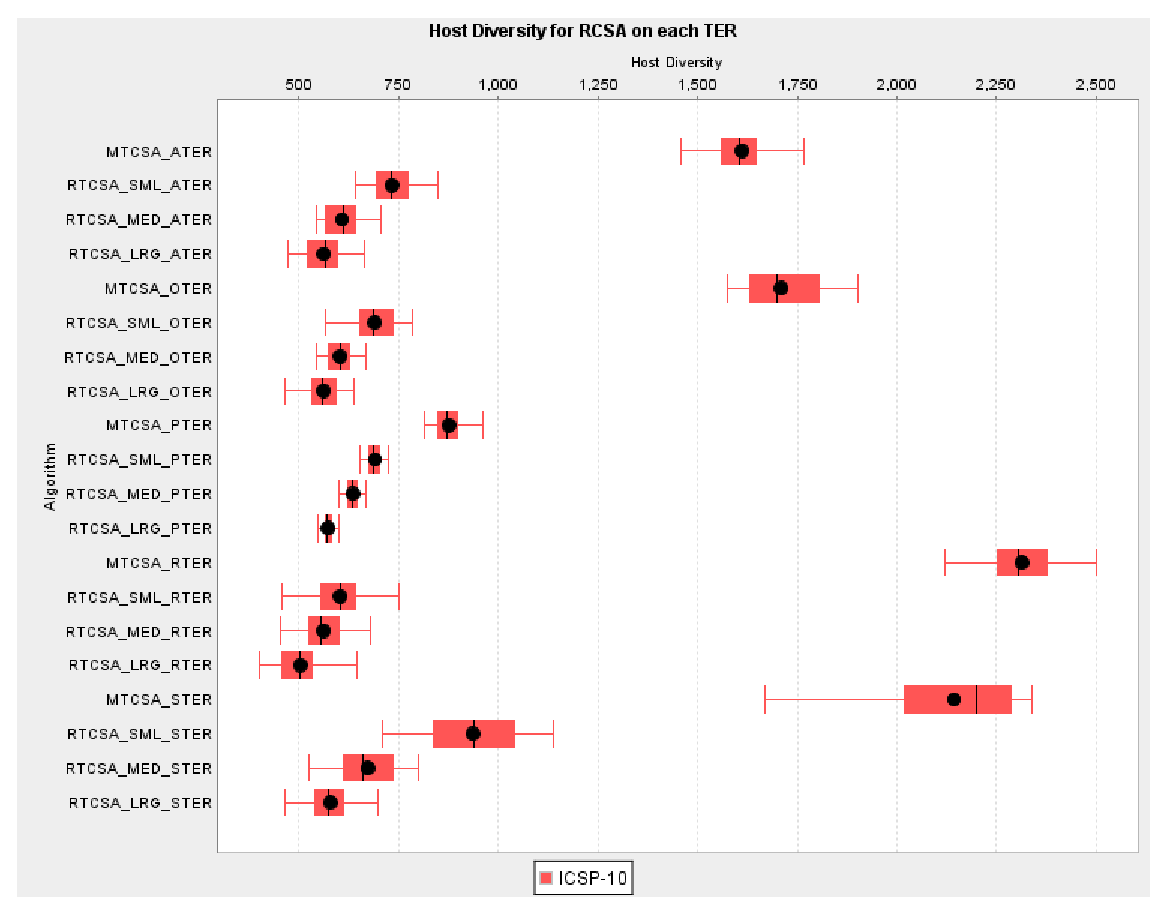
\includegraphics[scale=0.65]{Tissues/RTCSA-HD}
	\caption{Box-and-whisker plot of Host Diversity (HD) across all TER for the RTCSA study.}
	\label{fig:tissues:rtcsa:hd:boxplot}
\end{figure}

\begin{figure}[htp]
	\centering
		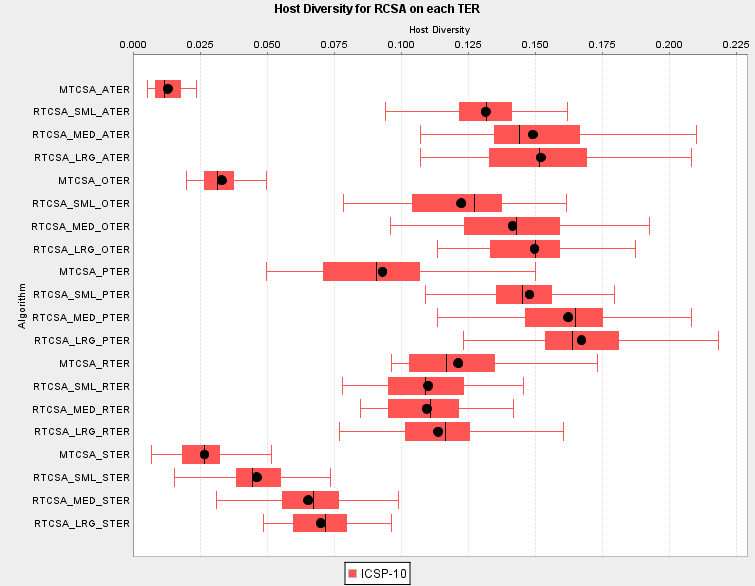
\includegraphics[scale=0.65]{Tissues/RTCSA-HE}
	\caption{Box-and-whisker plot of Host Error (HE) across all TER for the RTCSA study.}
	\label{fig:tissues:rtcsa:he:boxplot}
\end{figure}

\begin{figure}[htp]
	\centering
		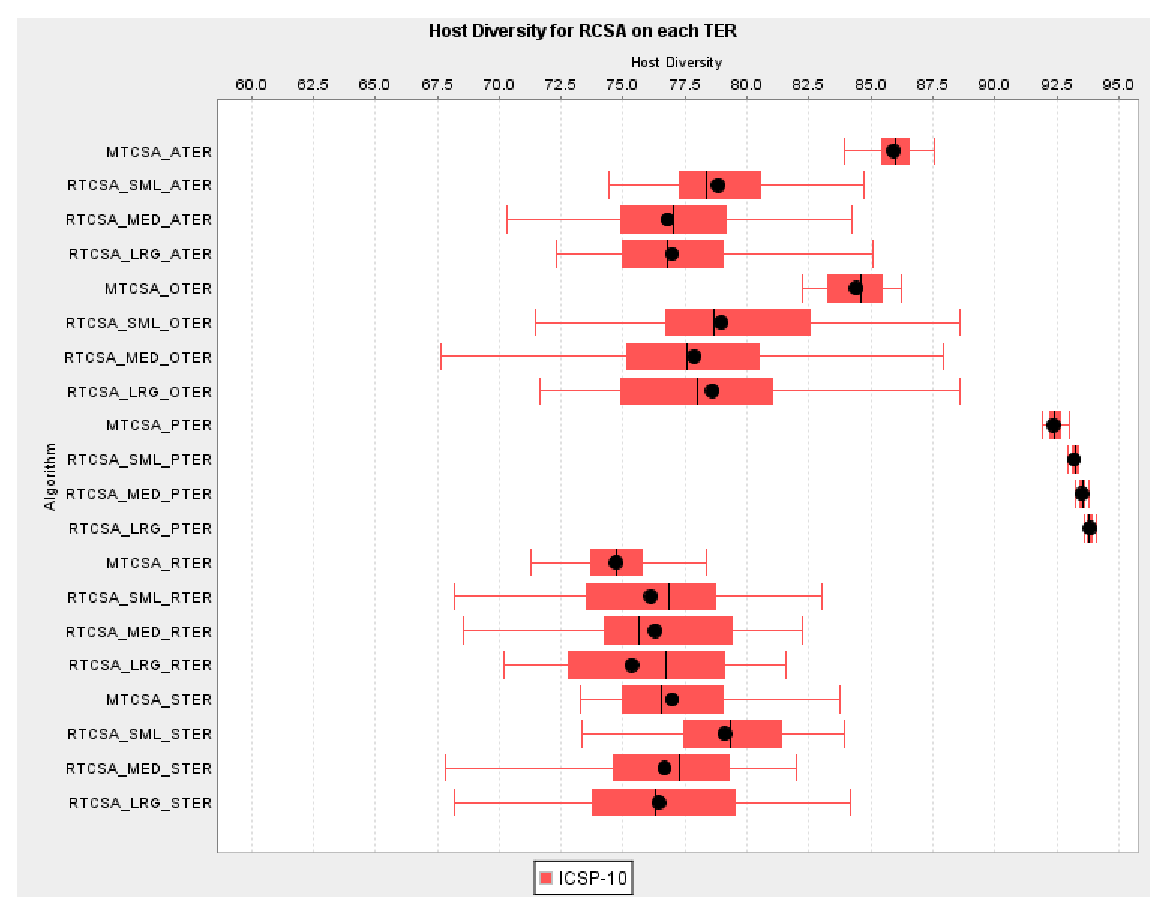
\includegraphics[scale=0.65]{Tissues/RTCSA-ATD}
	\caption{Box-and-whisker plot of Average Tissue Diversity (ATD) across all TER for the RTCSA study.}
	\label{fig:tissues:rtcsa:atd:boxplot}
\end{figure}

\begin{figure}[htp]
	\centering
		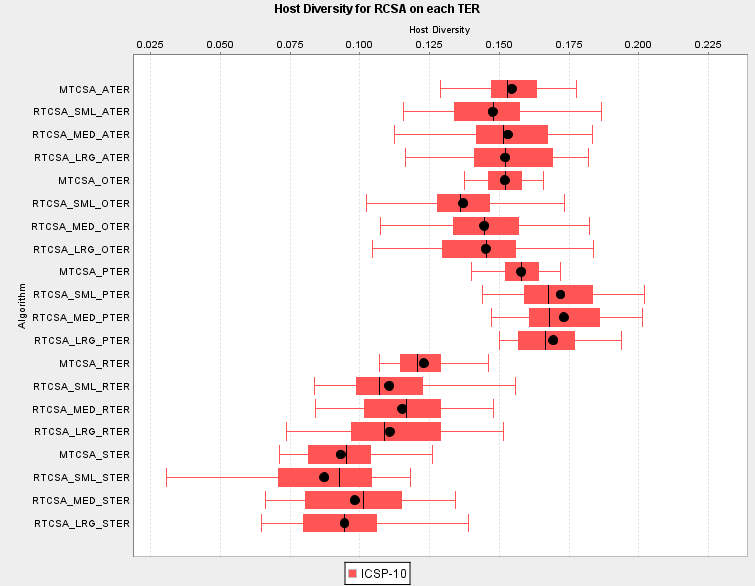
\includegraphics[scale=0.65]{Tissues/RTCSA-ATE}
	\caption{Box-and-whisker plot of Average Tissue Error (ATE) across all TER for the RTCSA study.}
	\label{fig:tissues:rtcsa:ate:boxplot}
\end{figure}

%
% Analysis
%
\subsubsection{Analysis}
This section provides an analysis of the results summarises in the previous section. Table~\ref{tab:tissues:trends:exposure:behaviour} was used to consider the general behaviour of each of the specific TER's. Table~\ref{tab:tissues:trends:mechanism:behaviour} was used to consider the general behaviour of the global and local information management strategies of RTCSA and MTCSA. Finally, Table~\ref{tab:tissue:measures:interpretation:trends} was used to qualitative interpret the summarised results.

%
% Information Management Trends
%
\paragraph{Information Management Trends}
This section considers the expected trends of the local and global information management trends under local and global information exposure regimes outlined in Table~\ref{tab:tissue:measures:expected:behaviour} from Section~\ref{subsec:tissues:paradigm:method:behaviours}. ATER and RTER are considered local and global information exposure regimes (exposure and re-exposure) respectively, and MTCSA and RTCSA-LRG are considered local and global information management (anticipation) respectively. Table~\ref{tab:tissue:rtcsa:trends} provides a variation on the expected trends summary presented in Table~\ref{tab:tissue:measures:expected:behaviour} in which the specific measures of the selected algorithms are provided with qualitative comparison. Direct comparison between these tables addresses the primary aim of the experiment, to confirm or reject the behaviour expectations outlined in the tissue paradigm agenda in Section~\ref{subsec:tissues:paradigm:method:agenda}.

\begin{table}[ht]
	\centering\small
		\begin{tabular}{lllllll}
		\toprule
		\textbf{Measure} & \multicolumn{3}{c}{\textbf{ATER}} & \multicolumn{3}{c}{\textbf{RTER}} \\ 
		\midrule
		 				 & \emph{RTCSA-LRG} & \emph{MTCSA} & Sig. & \emph{RTCSA-LRG} & \emph{MTCSA} & Sig. \\ 
		\toprule
		\emph{HD}  & 562.136 ($\downarrow$) & 1610.68 ($\uparrow$) & True & 503.919 ($\downarrow$) & 2313.88 ($\uparrow$) & True\\ 
		\emph{HE}  & 0.152 ($\uparrow$) & 0.013 ($\downarrow$) & True &  0.114 ($\downarrow$) & 0.121 ($\uparrow$) & False \\ 
		\emph{ATD} & 76.969 ($\downarrow$)  & 85.903 ($\uparrow$) & True & 75.347 ($\uparrow$) & 74.7 ($\downarrow$) & False \\ 
		\emph{ATE} & 0.152 ($\downarrow$) & 0.155 ($\uparrow$) & False & 0.111 ($\downarrow$) & 0.123 ($\uparrow$) & True \\  
		\bottomrule
		\end{tabular}
	\caption{Summary of the results for MTCSA and RTCSA-LRG on ATER and RTER and the relative quantitative difference is measures.}
	\label{tab:tissue:rtcsa:trends}
\end{table}

% local exposure
Considered first are the algorithm results for the local information exposure regime (ATER). 
% system
From a system perspective both the HD and HE met the expectations in which the MTCSA resulted in decreased error and increased diversity, whereas the RTCSA-LRG resulted in the inverse behaviour of increased error and decreased diversity.
% component
From a component perspective the comparison in diversity (ATD) did not meet expectations. Instead of an increase in average component diversity with a global strategy, this behaviour was observed by the local strategy. This means that the expectation that the global strategy would decrease component specialisation was interpreted incorrectly, demonstrating that a general increase in specialisation with a local strategy results in an increase in the diversity within the average component. Also unexpected was the lack of significant difference between the average component error between the two strategies. This was a surprising result as the mixing of acquired information provided by RTCSA-LRG provided no measured performance improvement over segregated repertoires on the local exposure regime.

% global exposure
The algorithm results from the global information exposure regime (RTER) are also considered.
% system
From a system perspective the diversity matched the expectation in which the segregation of MTCSA resulted in an increase in diversity compared to the decreased provided by recirculation in RTCSA-LRG. The expectation that system error would decrease with RTCSA-LRG was not confirmed as there was no significant difference between the two strategies. This is a surprising result as it generally suggests that consistency of response may not improve system performance under an irregular global information exposure regime\footnote{This suggestion is further supported by the lack of significance between MTCSA and all tested variations of RTCSA on RTER as shown in Table~\ref{tab:tissues:rtcsa:results}.}. 
% component
From a component level the expectation of component error was confirmed in which the global strategy resulted in a decrease in HE compared to an increase seen with the local strategy. The expectation of component diversity was not confirmed as their was no significant difference between the two strategies. This finding, together with the lack of significant difference in HE demonstrates that RTER alone was sufficient to engender a `consistency of response' irrespective of the information management strategy, promoting a reconsideration of cause and effect between management strategies and exposure regimes. This is considered in the remainder of this section.
% re-do the table, highlighting the differences 
Table~\ref{tab:tissue:rtcsa:expected:confirmed} provides a reproduction of the expectations from Table~\ref{tab:tissue:measures:expected:behaviour} of global and local information management strategies and information exposure regimes, with those results that did not meet the expectations highlighted.

\begin{table}[ht]
	\centering\small
		\begin{tabular}{llllll}
		\toprule
		\multicolumn{2}{c}{Measure} & \multicolumn{2}{c}{Local-Local TER} & \multicolumn{2}{c}{Global-Global TER} \\ 
		\midrule
		\emph{Scope} & \emph{Type} & \emph{Global Strategy} & \emph{Local Strategy} & \emph{Global Strategy} & \emph{Local Strategy} \\ 
		\toprule	
		\emph{System} & \emph{Diversity} 	  & Decreased & Increased & Decreased & Increased \\ 
		\emph{System} & \emph{Error} 			  & Increased & Decreased & \textbf{Neutral} & \textbf{Neutral} \\ 		
		\emph{Component} & \emph{Diversity} & \textbf{Decrease} & \textbf{Increase} & \textbf{Neutral} & \textbf{Neutral} \\ 
		\emph{Component} & \emph{Error}  	  & \textbf{Neutral} & \textbf{Neutral} & Decreased & Increased \\ 
		\bottomrule
		\end{tabular}
	\caption{Summary of confirmed behaviours of global and local information strategies and exposure regimes, highlighting where expectations were incorrect.}
	\label{tab:tissue:rtcsa:expected:confirmed}
\end{table}

%
% Information Exposure Trends
%
\paragraph{Information Exposure Trends}
This section relaxes the notions of local and global information exposure regimes and considers general trends across the TER's in the context of both the local and global management strategies (MTCSA and RTCSA-LRG respectively). Table~\ref{tab:tissues:rtcsa:results:ter} in Appendix \ref{appendix:results:tissues:recirculation} provides a restricted summary of results that provides direct comparison and statistical significance between TER's for the local and global management strategies in which the effects of the exposure regimes may be teased from their information management strategies. 

% local strategy
Observations may be drawn firstly from the behaviour of the five TER's with the local management strategy (MTCSA). 
% system
From a system perspective, PTER resulted in the least diverse system whereas RTER resulted in the most diverse system. This suggests that the holistic adaptation the system was exposed to in RTER and other system-wide exposure regimes (ATER, STER and OTER) result in a system information content that is more diverse than the random repertoires under PTER (besides the single exposed tissue). ATER achieved the lowest error, which is unsurprising given the $T$-$I$ specialisation fostered by the TER, and RTER achieved the highest error which was also expected given it provides the least $T$-$I$ specialisation (the most irregular regime).
% component
From a component level, PTER achieved the highest ATD and ATE\footnote{Difference in ATE was not significant between PTER and ATER for MTCSA.} suggesting that from a component perspective point-wise exposure of information results in the expected behaviour of repertoires that individually perform poorly on average. This behaviour was not restricted to PTER as was also demonstrated to a lesser degree on the other restricted exposure regimes (ATER and OTER). RTER resulted in the lowest average component diversity, although with similar behaviour exhibited by STER, suggesting system-wide exposure of information results in repertoires that have consistent internal information content on average. STER achieved the lowest ATE followed by RTER demonstrating that the same effect on component diversity results in improved tissue capability.

% global strategy
Observations may be summarised from the behaviour of the five TER's with the global management strategy (RTCSA-LRG). 
% system
From a system perspective STER resulted in the lowest diversity and error. RTER resulted in the highest diversity although was not significantly different from many of the other TER's. Interestingly, PTER resulted in the highest error suggesting that global management presented a major disruptive influence to localised exposure regimes, demonstrated by the equally poor HE for ATER and OTER compared to the much improved STER and RTER. Further, this inverse in behaviour from the local management strategy results demonstrate the suitability of holistic exposure regimes to the global management strategy, and localised exposure regimes to the local management strategy.
% component
From a component level, PTER achieved the highest average component diversity and error demonstrating the same trend with the MTCSA management strategy. RTER resulted in the lowest ATD with no significant difference in result with the STER and ATER system-wide exposure regimes. Likewise STER resulted in the lowest ATE followed closely by RTER mirroring the pattern observed with MTCSA.

Toward teasing apart the influences of TCSA's and TER's the observations may be reduced into the following trends that describe the generalised relationship between information exposure strategy and information management strategy:

\begin{enumerate}
	% components
	\item \emph{Component Trends are Strategy Invariant}
	\begin{enumerate}
		\item Localising information exposure increases average component diversity, globalising information exposure decreases average component diversity.
		\item Localising information exposure increases average component error, globalising information exposure decrease average component error.
	\end{enumerate}
	% system
	\item \emph{System Trends are Strategy Variant}
	\begin{enumerate}
		\item Globalising information management increases diversity and error under localised information exposure, and decreases diversity and error under globalised information exposure.
		\item Localising information management decreases diversity and error with localised information exposure, and increases diversity and error with a globalised exposure strategy.
	\end{enumerate}
\end{enumerate}

% component implications
The component measure invariance trend with information management strategy demonstrates that the information exposure regime is the determining factor. This trend was observed independently for both the MTCSA and RTCSA-LRG strategies across the TER's, although specific and typically minor differences for strategies on specific TER's.
% system implications
The system measure dependence on information management strategy demonstrates the suitability of a localised strategy on localising information exposure and the suitability of a globalised strategy on globalising information exposure. This trend was observed independently and complementary (the inverse case) for both MTCSA and RTCSA-LRG strategies across the TER's, although with differences in the specific TER in each case.
% the link
An important implication regarding TER's in addition to that of their spatial-temporal regularity is the scope of their exposure behaviour as either system-wide or restricted, providing a defining quality for localisation and dissemination management strategies.
% relation to algorithms
These trends suggest that TER's can predictably influence the component-wise organisation of information in terms of holistic problem error and information content diversity. The system-level suitability trends also suggest that MTCSA does demonstrate the spatial organisation (localisation) of information emergent effect and that RTCSA-LRG does demonstrate the consistency of response (dissemination) emergent effect, confirming the expectations regarding each approaches mechanism. 

%
% Recirculation Trends 
% (likely the most scrappy of the analysis)
%
\paragraph{Recirculation Trends}
This section considers information management strategies beyond the two extremes already considered. Specifically, this section considers the range of recirculation sample sizes ($N_{migration}$) as intermediates between the two extremes, across all five TER's. These recirculation trends are drawn from the principle result summarises, specifically Table~\ref{tab:tissues:rtcsa:results}, and Figures \ref{fig:tissues:rtcsa:hd:boxplot}, \ref{fig:tissues:rtcsa:he:boxplot}, \ref{fig:tissues:rtcsa:atd:boxplot} and \ref{fig:tissues:rtcsa:ate:boxplot}. 

% system-diversity
From the system perspective, migration size demonstrated the consistent trend of decreasing diversity (HD) where the larger the sample size the larger the decrease in HD compared to MTCSA. 
% system-error
A consistent trend was also demonstrated with error, where the increase in recirculation size resulted in increased system error compared to MTCSA. This generalised error trend applied to all TER's with system-wise exposure scope (all tissues participated, not PTER). These system-level diversity and error trends provide clear intermediates in system-level behaviour (localisation and dissemination) as defined by the captured measures HD and HE.
% component
From a component perspective the trends are less bold as a the system level.
% component diversity (sweet spot)
ATD demonstrate no clear TER invariant trends with recirculation size, although there was clear commonality in behaviour. For both the ATER and OTER exposure regimes, the increase in recirculation size resulted in a step decrease in average component diversity that seemingly levelled off after the drop from MTCSA to RTCSA-SML. This demonstrates that a sufficiently small sample size was required to effect a decrease in the average tissue diversity under those regimes, after which further increases in sample size had little effect. Interestingly, a different effect was observed for RTER and STER where a small recirculation size resulted in a small increase in ATD, after which further increases in size resulted in decreases. 
These effects were not observed with PTER, where the increase in recirculation size resulted in the progressive increase in ATD.
% component error
The variation in recirculation size demonstrated a common trend across all TER's except PTER for ATE, where a small increase resulted in a decreased error, and subsequently larger recirculation sizes increased error. This trend demonstrates that a sufficiently small recirculation size is needed to effect a drop in AE under those exposure regimes. The inverse of this trend was observed with PTER where small recirculation resulted in an increase in ATE and larger sample sizes decreased this error toward the MTCSA score.

% generalisation
The observed measure-based may be reduced into the following generalised trends regarding RTCSA recirculation size:

\begin{enumerate}
	\item \emph{Graceful Intermediate Dissemination Effect}
	\begin{enumerate}
		\item The RTCSA recirculation size provides a graceful intermediate in emergent behaviour (system-level) between localisation demonstrated in MTCSA and dissemination.
		\item Small recirculation size provides a decrease in average component error where large recirculation sizes do not on system-wide exposure regimes with local and global re-exposure.
		\item Recirculation decreases the diversity of the average component on system-wide exposure regimes with local re-exposure.
		\item Recirculation increases the diversity of the average component on system-wide exposure regimes with global re-exposure.
	\end{enumerate}	
\end{enumerate}

% NOTE: the variations on the component trends is a product of the strategy invariance - determined by the exposure regime


%
% Conclusions
%
\subsubsection{Conclusions}
This section summarises the findings of the empirical study into the Recirculation Tissue Clonal Selection Algorithm, in terms of the primitives that were the focus of the study and the expectations that motivated the study.

\begin{enumerate}
	% primitives
	\item \emph{Study Primitives}
		\begin{enumerate}
			\item The MTCSA is a viable realisation of the spatial organisation effect (localisation) via an isolation mechanism.
			\item The RTCSA is a viable realisation of the consistency of response effect (dissemination) via a recirculation mechanism.
		\end{enumerate}
	
	% findings
	\item \emph{Confirmations and Findings}
		\begin{enumerate}
			\item The behavioural expectations for the two different management strategies under two archetype exposure regimes were considered with a mixture of system and component level expectations being confirmed and rejected.
			\item The localisation or globalisation (exposure/re-exposure) of an exposure regimes defines the component-level error and diversity that is generally invariant to the information management strategy			
			\item The localisation or globalisation of an exposure regime is suited to a localising and disseminating information management strategy with regard to system-level error and diversity.
			\item In addition to the regularity and holistic information exposure/re-exposure properties of tissue exposure regimes, a third important consideration is the scope of system exposure, specifically system-wide or constrained exposure/re-exposure.
		\end{enumerate}	
	
	% intermediates
	\item \emph{Intermediates}
		\begin{enumerate}
			\item Recirculation size of the RTCSA provides a viable behavioural intermediate between localisation and dissemination with predictable systemic effects and identified component tends on varied exposure regimes.
			\item There is a need for a system to balance localisation and globalisation of acquired information when presented with an \emph{unknown} exposure regime.
		\end{enumerate}		
\end{enumerate}

% next section...
This final point about intermediates motivates the two remaining investigations in this chapter, and likely the whole Tissue Clonal Selection Paradigm.

%
% Homing
%
\section{Lymphocyte Homing}
\label{sec:tissues:homing}

%
% Homing Metaphor and Strategy
%
\subsection{Homing Metaphor and Strategy}
% metaphor
Section~\ref{subsec:tissues:migration:mobility} considered the directed trafficking of cells, with the specific example of the imprinting of T-cells by dendritic cells as to the chemical properties of a site of infection. The educated cells then recirculate until they locate the imprinted chemical signature and seek their cognate antigen.
% strategy
The RTCSA demonstrated that continual lymphocyte migration provides a background disruptive behaviour to a tissues ability to specialise a response to regular exposures. The education and homing mechanism for cells may be generalised to a specialisation of recirculation that empower cells to express a preferential residence in tissues for which they may be useful. This bottom-up behaviour is called a \emph{Preferential Residence Strategy} and is comprised of \emph{Cell Imprinting} and \emph{Differential Migration} mechanisms to realise the emergent effect.

% abstraction - imprinting
In addition to specialising the resources of the system to the antigenic exposures, the specialised resources (lymphocyte receptors for antigen) must be positioned such that they are used in the right locations. The distribution (space and time) of antigenic exposures is unknown to the system (defined by a TER), thus the system recirculates specialised resources between the locations of exposure to maximise the chance application of the resource in an exposure event. Lymphocytes interact with each other and interact with antigen in this spatial structure. Each tissue type associated with a region of the host has its own unique chemical makeup, which may be used to differentiate tissues types and thus regions of the host. Lymphocytes may interact with tissues using specialised receptors that detect and differentiate between tissue types. This interaction occurs when the lymphocyte recirculates around the host, and may be used by the cell to travel specific pathways and to enter and remain in a specific tissue in search of its cognate antigen. These navigation receptors are not expressed in \naive\ lymphocytes, instead are expressed in matured cells that are produced after an interaction with antigen. A mature receptor (memory or effector) expresses navigation receptors for the tissue surroundings when it is conceived. Therefore, mature cells are specialised both for an antigenic stimulus, and for the spatial location (tissue) that is known to have been exposed to the antigenic stimulus. This \emph{Cell Imprinting} process occurs irrespective of whether a selected (high-affinity) lymphocyte is mature or \naive. In effect, specialised resources may be re-educated in that their progeny may be imprinted with a different location than themselves (presuming the cell was selected in a tissue different from that it may home to). This imprinting mechanism facilitates both the spatial anticipation of antigen exposure based on past exposures, and in addition to recirculation, it facilitates the use and re-education of lymphocytes. 

% abstraction - differential migration
Imprinting empowers individual mature lymphocytes to assert preference for their locations allowing tissues to discriminate preferential residence during the selection of cells to traffic. Homing requires an imprinting apparatus, which includes both a unique identity or signature for tissues, and a way for lymphocytes to be impregnated with that signature. The match of information between a given lymphocyte and a tissue may be used to bias the selection of cells from the repertoire to migrate. One may consider a Boolean match/no-match for lymphocytes in their home tissue, and those not in their home tissue. Those progeny lymphocytes created as a result of the clonal selection process are already in their home tissue, thus they have a match to their tissue's signature. All those lymphocytes that migrate from another tissue will not match. Thus, a migration sample selection policy that biases toward no-matches and away from matches (1) exercises a preference for lymphocytes (2) facilitates an automatic recirculation population of homeless lymphocytes. This process is called \emph{Differential Recirculation} where the probability that a mature lymphocyte is selected in an outbound migration sample is biased by the match between a given lymphocyte and the tissue's signature. This mechanism facilitates homing but introduces the problem of recruitment into the recirculation pool. Those cells in the recirculating pool will continue recirculating until they return their `home', unless they get used or killed elsewhere. The initial recruitment probability will be uniform across the repertoire as there are no migrant cells to consider. If a recirculating cell is replaced (killed) by the proliferation strategy at another (non-home) tissue, then that tissue will fill the gap in the recirculating population. 

%
% Homing Tissue Algorithm
%
\subsection{Homing Tissue Algorithm}
The Homing Tissue Clonal Selection Algorithm (HTCSA) is defined as an extension of the RTCSA with the addition of a cell imprinting and differential migration mechanisms. 

%
% Cell Imprinting
%
\paragraph{Cell Imprinting}
A pattern-recognition method may be used that is somewhat similar to the approach used for Mediated Cellular Clonal Selection (Section~\ref{sec:cells:mediated}) or Network Cellular Clonal Selection (Section~\ref{sec:cells:network}), although rather than a lymphocyte matching onto other lymphocytes with a mock `surface feature', lymphocytes are provided with an additional receptor for detecting and matching the tissue they are in. In keeping with the bitstring basis of the minimal clonal selection algorithm (and extensions), a simple and scalable method is to assign each tissue (or tissue group) a random binary string. Each mature lymphocyte (that is a lymphocyte created from a cloning and maturation process) is then assigned (imprinted) with a copy of the tissue bitstring specific to the location of its creation. A less elaborate approach involves assigning a distinct identification number to each $T$ in $H$ and assigning a tissues identification number to activated cells at the time of exposure. Algorithm~\ref{alg:tissues:algorithms:htcsa:imprinting} defines a generic tissue exposure function in which the cell repertoire is ordered by its affinity for an Antigen $A$ ($OrderByAffinity(T, C_i)$) and a subset of the $N_{imprint}$ highest affinity cells for $A$ are imprinted with the current tissue identification number.

\begin{algorithm}[ht]
  \SetLine
  \SetKwData{Infection}{I}
	\SetKwData{Tissue}{T}
	\SetKwFunction{OrderByAffinity}{OrderByAffinity}
	\SetKwFunction{Exposure}{Exposure}
	
  \KwIn{\Infection, \Tissue, $N_{imprint}$}		
  
	\ForEach{$A_i \in$ \Infection}
	{
		% expose repertoire to A_i
		\ForEach{$C_j \in$ \Tissue}
		{
			\Exposure{$C_j$, $A_i$}\;		
		}
		% imprint cells
		\OrderByAffinity{\Tissue, $C_i$}\;		
		\For{j$\leftarrow$1 \KwTo $N_{imprint}$}
		{
			$C_j$.TissuePreference $\leftarrow$ \Tissue.id\;
		}
	}
	\caption{Cell Imprinting for Homing Tissue Clonal Selection.}
	\label{alg:tissues:algorithms:htcsa:imprinting}
\end{algorithm}

%
% Differential Migration
%
\paragraph{Differential Migration}
The  $TissueInteractions(H)$ operation of the RTCSA that governed tissue interactions in the general TCSA may be specialised to exploit the imprinted cells by (1) migrating those cells that are not in their preferred tissue or do not have a preference, and not migrating those cells that are in their preferred tissue. Such preferences may be deterministic or probabilistically implemented. Algorithm~\ref{alg:tissues:algorithms:htcsa:differential} provides a re-definition of the $TissueInteractions$ defined for RTCSA in Algorithm~\ref{alg:tissues:algorithms:rtcsa} that simplifies differential migration by not migrating those cells in their preferred tissue. The $SelectSingleCell$ operation draws cells randomly from the $T$.

\begin{algorithm}[ht]
  \SetLine
  \SetKwData{Host}{H}
  \SetKwFunction{Integrate}{Integrate}
  \SetKwFunction{SelectSingleCell}{SelectSingleCell}
  
  \KwIn{\Host, $N_{migration}$}
	
	$H\prime \leftarrow 0$\;
	% collect samples
	\ForEach{$T_i \in$ \Host}
	{
		% preferential selection duration migration
		$T_{i}\prime \leftarrow$0\;
		\While{$T_{i}\prime_{N} \neq N_{migration}$}
		{
			$C\prime \leftarrow$ \SelectSingleCell{$T_i$}\;
			% exert preference
			\If{$C\prime$.TissuePreference $\neq T_i$.id}
			{
				$T_{i}\prime \leftarrow C\prime$\;
			}
		}
		$H\prime \leftarrow T_{i}\prime$\;
	}
	% transmit samples
	\ForEach{$T_{i}\prime \in H\prime \wedge T_i \in$ \Host}
	{
		\uIf{$T_i \equiv T_N$}
		{
			\Integrate{$T_{i}$, $T_{1}\prime$}\;
		}
		\Else
		{
			\Integrate{$T_{i}$, $T_{i+1}\prime$}\;
		}		
	}	
	\caption{Differential Migration for Homing Tissue Clonal Selection.}
	\label{alg:tissues:algorithms:htcsa:differential}
\end{algorithm}


%
% Homing Empirical Study
%
\subsection{Homing Empirical Study}
\label{sec:tissues:homing:study}
%
% Aim
%
\subsubsection{Aim}
The aim of this empirical study was to investigate the Homing Tissue Clonal Selection Algorithm (HTCSA) as an intermediate information strategy between high migration RTCSA and the segregated MTCSA. Toward this end, the study had the following goals:

\begin{enumerate}
	\item Contrast HTCSA against MTCSA and RTCSA as a mechanism for simultaneously promoting dissemination and localisation of acquired information.
	\item Investigate intermediates of the HTCSA mechanism and subsequent effect by varying the $N_{imprint}$ parameter.
\end{enumerate}


%
% Method
%
\subsubsection{Method}

%
% Algorithms
%
\paragraph{Algorithms}
The study considers three algorithms, the Minimal Tissue Clonal Selection Algorithm (MTCSA), and the Recirculation Tissue Clonal Selection Algorithm (RTCSA), and the Homing Tissue Clonal Selection Algorithm (HTCSA). 
% MTCSA
The MTCSA and RTCSA algorithm are configured as was defined for the RTCSA empirical study in Section~\ref{subsec:tissues:recirculation:study} with $N_{tissues}=10$, $N_{cells}=50$, $N_{selection}=1$, $N_{clones}=5$ for MTCSA and RTCSA, and $N_{migration}=5$ (10\% of each $T$) fixed for the RTCSA.
% HTCSA
HTCSA is an extension of RTCSA with the addition of an imprinting operation as defined in Algorithm~\ref{alg:tissues:algorithms:htcsa:imprinting} for each exposure and a differential migration as defined in Algorithm~\ref{alg:tissues:algorithms:htcsa:differential}. The imprinting mechanism was specialised such that a variable number $N_{imprint}$ of the best-matching cells were imprinted for each exposure, as follows: small (HTCSA-S) $N_{imprint}=1$ (2\% of $T$), medium (HTCSA-M) $N_{imprint}=5$ (10\% of $T$), and large (HTCSA-L) $N_{imprint}=10$ (20\% of $T$). A probabilistic sample selection scheme was used in differential migration, changing the configuration from 100\% rejection if a cell was housed within its `home' tissue to a probabilistic 20\% (80\% chance of home cells not being migrated per migrating cell selection). 

%
% Problems
%
\paragraph{Problems}
The same Infection Colour Space Problem and Tissue Exposure Regimes were used as was defined for the RTCSA empirical study in Section~\ref{subsec:tissues:recirculation:study}.

%
% Experiment
%
\paragraph{Experiment}
The same experimental setup was used as was defined for the RTCSA empirical study in Section~\ref{subsec:tissues:recirculation:study}.

%
% Results
%
\subsubsection{Results}
Table~\ref{tab:tissues:htcsa:results} in Appendix \ref{appendix:results:tissues:homing} provides a summary of results for each algorithm-problem combination including the mean ($\bar{x}$) and standard deviation ($\sigma$) of collected measure values. Box-and-whisker plots are provided in which the results for each algorithm are aggregated across all TER for a each measure. Figure~\ref{fig:tissues:htcsa:hd:boxplot} shows HD, Figure~\ref{fig:tissues:htcsa:he:boxplot} shows HE, Figure~\ref{fig:tissues:htcsa:atd:boxplot} shows ATD, and Figure~\ref{fig:tissues:htcsa:ate:boxplot} shows ATE.

\begin{figure}[htp]
	\centering
		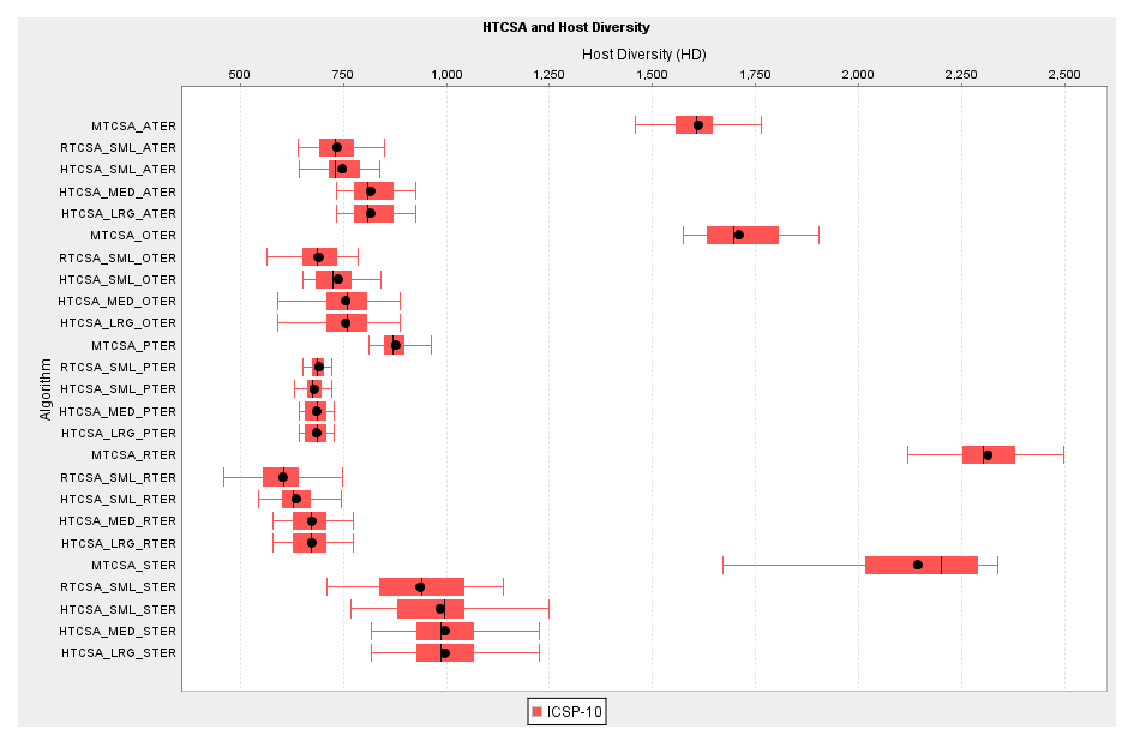
\includegraphics[scale=0.70]{Tissues/HTCSA-HD}
	\caption{Box-and-whisker plot of Host Diversity (HD) across all TER for the HTCSA study.}
	\label{fig:tissues:htcsa:hd:boxplot}
\end{figure}

\begin{figure}[htp]
	\centering
		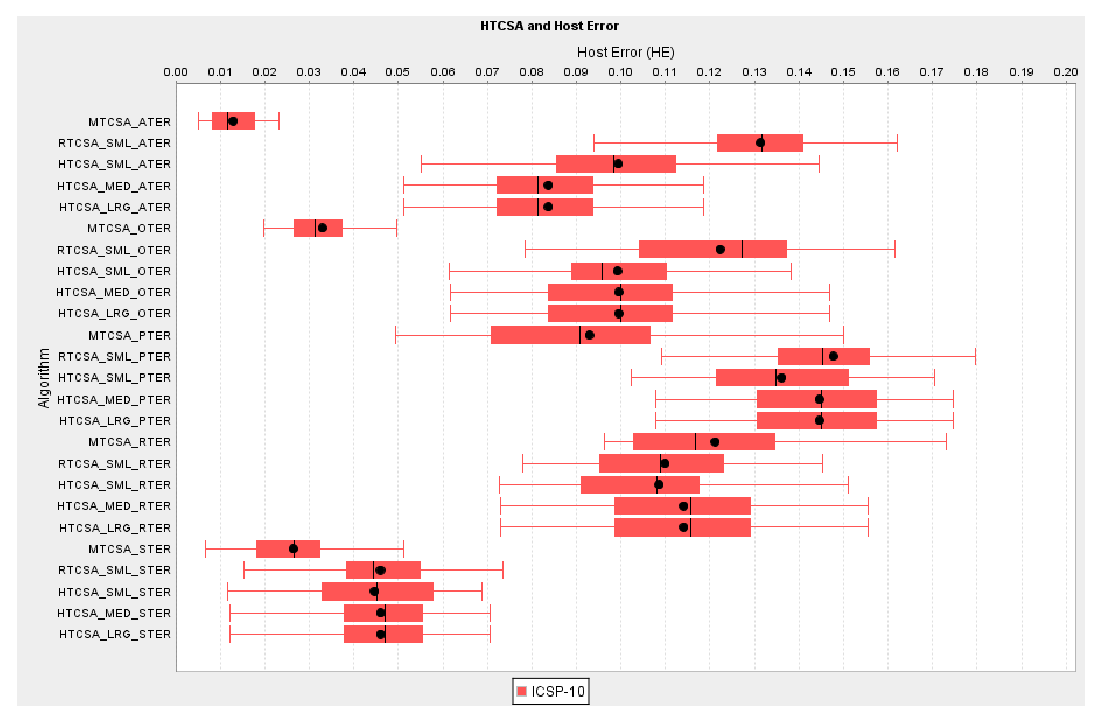
\includegraphics[scale=0.70]{Tissues/HTCSA-HE}
	\caption{Box-and-whisker plot of Host Error (HE) across all TER for the HTCSA study.}
	\label{fig:tissues:htcsa:he:boxplot}
\end{figure}

\begin{figure}[htp]
	\centering
		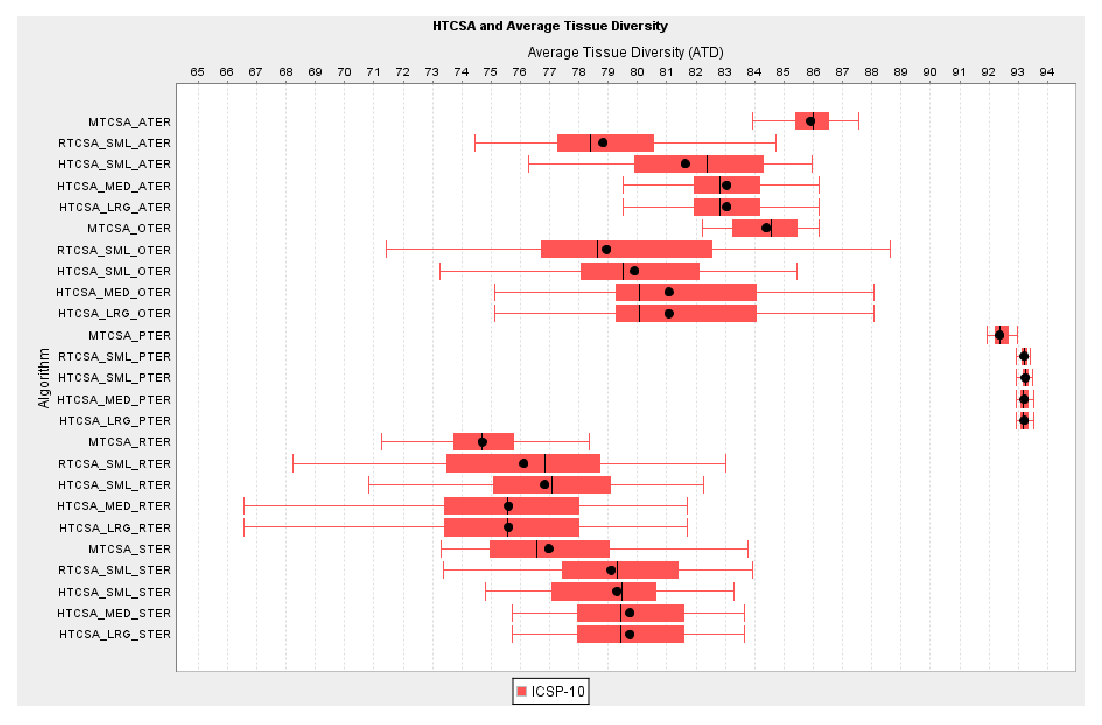
\includegraphics[scale=0.70]{Tissues/HTCSA-ATD}
	\caption{Box-and-whisker plot of Average Tissue Diversity (ATD) across all TER for the HTCSA study.}
	\label{fig:tissues:htcsa:atd:boxplot}
\end{figure}

\begin{figure}[htp]
	\centering
		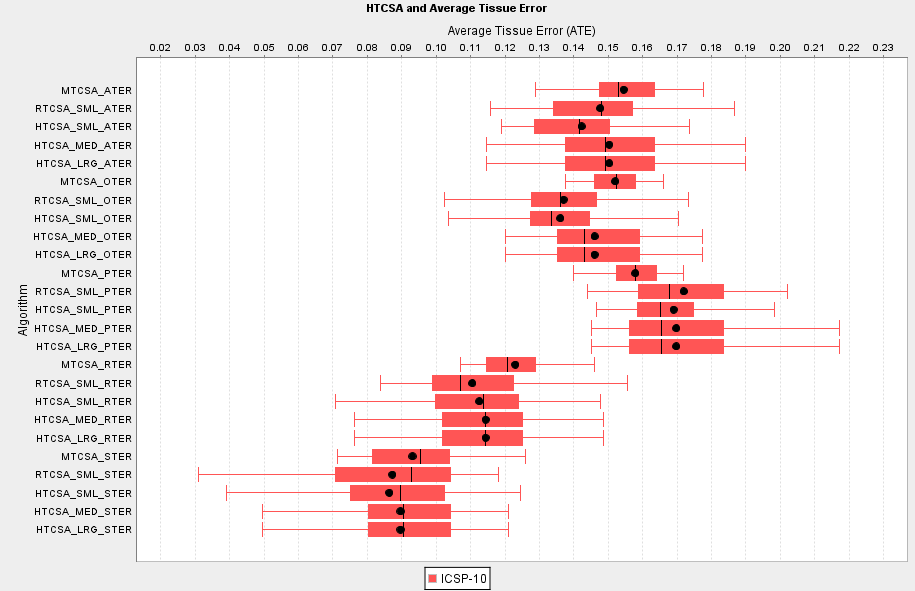
\includegraphics[scale=0.70]{Tissues/HTCSA-ATE}
	\caption{Box-and-whisker plot of Average Tissue Error (ATE) across all TER for the HTCSA study.}
	\label{fig:tissues:htcsa:ate:boxplot}
\end{figure}


%
% Analysis
%
\subsubsection{Analysis}
This section analyses the summarised results in Table~\ref{tab:tissues:htcsa:results} in the context of the expectations from Section~\ref{subsec:tissues:paradigm:method:behaviours} and their confirmation and other findings regarding MTCSA and RTCSA from the empirical study in Section~\ref{subsec:tissues:recirculation:study}.

%
% Localisation and Dissemination Trends
% HTCSA vs RTCSA vs MTCSA
%
\paragraph{Localisation and Dissemination Trends}
This section considers a comparison in behaviour between the the localising MTCSA, the disseminating RTCSA-S and preferential residence HTCSA-L. 
% system
From a system perspective HTCSA-L performed in a similar way to that as RTCSA-S, both of which were contrastingly different from MTCSA. Both RTCSA-S and HTCSA-L were less diverse than MTCSA, although RTCSA-S more so than HTCSA-L. MTCSA achieved consistently lower HE, although HTCSA-L demonstrated a decreased error on constrained exposure regimes (ATER, OTER and PTER) compared to RTCSA-S, and no significant difference in error on the remaining (RTER and STER) exposure regimes. This was an important finding highlighting the increased spatial organisation capability for recirculation with preferential residence over recirculation without preferential residence on regular exposure regimes.
% component
From a component perspective the performance of HTCSA-L was distinct from MTCSA and similar to RTCSA-S, with generally little significant difference in the use or non-use of preferential residence. ATD was increased in HTCSA-L over RTCSA-S for the same constrained exposure regimes in which an improvement in system error was observed (ATER, OTER and PTER), and no significant difference for the remaining regimes. This result highlights that under regular and constrained exposures (different information in different locations in a regular manner), preferential residence changes the composition of components toward that of segregated components, whilst under the presence of  recirculation, an effect that is not present for other exposure regimes. Specifically, preferential residence organises information toward the benefit of the system, when it is possible to do so as determined by the exposure regime. Homing had no consistent significant effect on recirculation regarding Average Tissue Error.
% trends
The observations comparing and contrasting the three strategies may be reduced to the following general behavioural trends for the preferential residence strategy:

\begin{enumerate}	
	\item Homing reduces system error over recirculation on constrained (regular) exposure regimes whilst remaining consistent with recirculation on irregular and system-wide exposure regimes.
	\item Homing increases system diversity (organisation) compared with recirculation.
	\item Decreased system error is reflected in increased average component diversity on constrained exposure regimes over recirculation, whilst remaining consistent with recirculation on irregular and system-wide exposure regimes.
	\item Improved organisation of homing does not effect average component error compared with recirculation.
\end{enumerate}

%
% Information Exposure Trends
%
\paragraph{Information Exposure Trends}
Section~\ref{subsec:tissues:recirculation:study} identified the two trends that (1) average component measures of error and diversity are defined by the localisation (constrained) or globalisation (system-wide) of the exposure (generally invariant to the information management scheme), and (2) that globalising management is suited to system-wide exposure regimes (global-global) and localising management is suited to constrained exposure regimes (local-local). This section considers the HTCSA in the context of these trends, specifically the degree to which the trends hold or are influenced by preferential residence. Table~\ref{tab:tissues:htcsa:results:ter} summarises results for HTCAS-L across all the TER's, providing a complement to the same presentation for MTCSA and RTCSA-L in Table~\ref{tab:tissues:rtcsa:results:ter}.

\begin{table}[ht]
	\centering\small
		\begin{minipage}{\textwidth} 
		\begin{tabular}{llllllllll}
		\toprule
		\textbf{System} & \textbf{Problem} & \multicolumn{2}{c}{\textbf{HD}} & \multicolumn{2}{c}{\textbf{HE}} & \multicolumn{2}{c}{\textbf{ATD}} & \multicolumn{2}{c}{\textbf{ATE}} \\ 
		\midrule
		TCSA & TER & $\bar{x}$ & $\sigma$ & $\bar{x}$ & $\sigma$ & $\bar{x}$ & $\sigma$ & $\bar{x}$ & $\sigma$ \\ 
		\toprule
		HTCSA-L & ATER & 816.023 & 53.374 & 0.084 & 0.019 & 83.046 & 2.228 & 0.15 & 0.018 \\ 
		HTCSA-L & OTER & 756.301 & 64.802 & 0.1 & 0.019 & 81.077 & 3.568 & 0.146 & 0.015 \\ 
		HTCSA-L & PTER & 685.395 & 27.472 & 0.145 & 0.017 & 93.206 & 0.161 & 0.17 & 0.018 \\ 
		HTCSA-L & RTER & 673.063 & 58.672 & 0.114 & 0.022 & 75.595 & 3.745 & 0.114 & 0.018 \\ 
		HTCSA-L & STER & 995.975 & 114.778 & 0.046 & 0.013 & 79.731 & 2.071 & 0.09 & 0.022 \\ 
		\multicolumn{2}{l}{Significance} & True\footnote{False for PTER and RTER} & & True & & True\footnote{False for STER and OTER} & & True\footnote{False for ATER and OTER} & \\ 
		\bottomrule
		\end{tabular}
		\end{minipage}
	\caption{Summary of results from an empirical study into the HTCSA comparing TER's with the HTCSA-L information management strategy.}
	\label{tab:tissues:htcsa:results:ter}
\end{table}

The results show the same trend with HTCSA-L as was shown with recirculation with a larger sample size in Table~\ref{tab:tissues:rtcsa:results:ter} (RTCSA-LRG rather than RTCSA-SML that would be a fair comparison with any assessed HTCSA). This confirmation supports the comparisons of RTCSA, MTCSA, and HTCSA and outcomes in the previous section. Specifically demonstrating that the influence of the TER's on the system remained generally consistent with RTCSA, and that the differences between RTCSA and HTCSA are as a result of the HTCSA strategy.


%
% Imprinting Size Trends
%
\paragraph{Imprinting Size Trends}
This section considers the intermediate effects of varying the number of cells imprinted with each exposure ($N_{imprint}$), and thus the extent of each tissue that is empowered to express a preference during migration.
% system
From a system perspective some preferential residence was better than none, although the increases in $N_{imprint}$ generally did not have a measurable effect. This result was generally demonstrated for both Host Error and Diversity across all exposure regimes except PTER. The Point Exposure Regime demonstrated a clear and steady increase in the organisation effect of preferential residence with the increase in the number of cells imprinted per exposure. This suggest that homing can counter the disruptive effects of recirculation, a behaviour that gracefully increases with the number of imprinted cells per exposure. This effect is most pronounced with PTER because it is the regime that is the most susceptible to the disruptive effects of blind recirculation.
% component
From a component perspective a similar general result was observed for average component diversity where preferential residence increased diversity with little difference between the value of $N_{imprint}$, and only on the ATER and OTER regimes with no significant effect on the other regimes. No consistent significant effect was observed for average component error in varying $N_{imprint}$, including a value of zero (RTCSA-S).
% trends
The observations regarding the variation of the number of imprinted cells per exposure may be generalised to the following trends: 

\begin{enumerate}
	\item Homing is generally better than no homing (recirculation) and the specific choice of $N_{imprint}$ is not critical.
	\item Increase in effect with increase in $N_{imprint}$ is pronounced on constrained local exposure (PTER), although is not significant under other exposure regimes.
\end{enumerate}

% future
An interesting consideration for future investigation is the correlation of decreased system diversity and increased system error with migration size, and the general increase in organisation and decrease in error with preferential residence. In particular the knowledge that the homing effect does scale when isolated in PTER. One may investigate the relationship between the recirculation size ($N_{migration}$) and the imprint size ($N_{imprint}$) in order to find general configuration trends toward a trade-off and balance of the dissemination and preferential organisation effect.

%
% Conclusions
%
\subsubsection{Conclusions}
This section summarises the findings of the empirical study into the Homing Tissue Clonal Selection Algorithm, in terms of the primitives that were the focus of the study and the expectations that motivated the study.

\begin{enumerate}
	% homing
	\item \emph{Homing}
		\begin{enumerate}
			\item The preferential residence (homing) effect realised in the imprinting and differential migration mechanisms provides a strategy that can exploit the dissemination of information by recirculation whilst countering the effect by localising used information.
			\item Cell localisation (20\% of a repertoire) is insufficient to counter all of the disruptive effects of continuous recirculation. 
			\item Localising used information allows progeny of such information to freely (blindly) recirculate.			
		\end{enumerate}			
\end{enumerate}

This final point provides a suggestion as to the basis of the mechanism in the homing approach, and a basis for increasing the probability of migration for cells without a preference. The second important finding for the homing approach (besides it behaving as intended) is that even with a large number of cells imprinted each exposure, it is unable to completly counter the disruptive effects of continuous recirculation, rather it is limited to complementing the process. Countering the disruptive effects would likely require the imprinting of some or all of the progeny of exposures, which is expected to impact the dissemination properties of recirculation. This theme of allowing sufficient specialisation under regular exposure regimes whilst also disseminating acquired information is further explored via a Tissue Inflammation metaphor in the next section.

%
% Inflammation
%
\section{Tissue Inflammation}
\label{sec:tissues:recruitment}

%
% Inflammation Metaphor and Strategy
%
\subsection{Inflammation Metaphor and Strategy}
% metaphor
When a tissue is infected by a pathogen that damages the local area, the response is inflammation at the site. Inflammation has many symptoms, not limited to swelling and the increased carrying capacity of lymphocytes in the tissue. In addition, the blood vessels that lead to the area dilate, increasing the flow of lymphocytes (information) to the site, and typically involves the use of chemical signals or attract recirculating cells and/or arrest cell movement. An increase in carrying capacity allows more lymphocytes created at the site of infection to remain there, and more cells to migrate and home into the tissue and collect at the site of infection. 
% strategy (specialised recruitment)
Inflammation provides a mechanism to temporally decrease the competition between lymphocytes for limited resources within a tissue, providing a tissue-level \emph{direct recruitment mechanism}. 
% abstraction (generalised recruitment)
One may consider the tissue paradigm from the perspective of active distributed recruitment strategies as opposed to passive distributed information organisation strategies (already considered). Information is streamed from the tertiary tissue to the secondary tissue although the streaming is facilitated by courier cells. These cells are aware of where they collected their material and thus are capable of imprinting that information onto the produced effector cells. The result is an effect that differentiates the lymphocyte movement behaviour from that of \emph{Recirculation} where cells blindly seek their cognate antigen, and from \emph{Homing} where cells home into the chemical signature of infected tissue. The Homing model couriers information about the location of the pathogen invasion to the cells which are imprinted with that information. This is a `fire and forget' response strategy. Like the recirculating of effectors, the homing effectors recirculate the system in search of their cognate antigen, although if the cells detect the imprinted signature of the site of infection, they take up residence and provide a local search strategy. Further, less effectors are created than in the recirculation model (for example mature T-cells as opposed to antibodies), thus the response is both smaller and more directed. One may generalise two response strategies as follows:

\begin{itemize}
	\item \emph{Undirected Response}: Flood the system with effectors that will generally address the specific site of invasion and any other sites where the pathogen may have spread, or penetrated on multiple fronts (recirculation method).
	\item \emph{Directed Response}: Produce a smaller set of effectors that home into the specific site of infection, and have a low chance of addressing additional sites of infection (homing method).
\end{itemize}

Both the undirected recirculation model and the directed homing model allocate (recruit) resources to the requirements of a specific antigenic exposure. Further, both strategies address the needs of the distributed information environment (resident receptors and inbound pathogen information). These two approaches may be considered to describe \emph{Distributed Recruitment Strategies}. The undirected approach is a flooding strategy that does not use any structural information other than the generation of a response in the vicinity of the pathogens first detection. The directed approach is a homing strategy in which structural information is used directly to get the resources to where they are required. Recruitment may be phrased as resource allocation with the desire of maximising payoff. Thus, \emph{Distributed Recruitment} may be defined as a strategy in which information dispersed across a spatial structure is sought (for example selected) and employed for a specific task (antigen neutralisation). The two proposed models both relate to the changing of lymphocyte trafficking behaviour, treating the lymphocyte (a space in the repertoire) as a limited resource. 

%
% Inflammation Tissue Algorithm
%
\subsection{Inflammation Tissue Algorithm}
% general properties about making it an algorithm
Inflammation is a strategy that promotes making more information available in the local area to address the infection, and there relaxing the competition between receptors for limited positions in the repertoire. This effect may be realised by temporary increasing the capacity of a tissue for lymphocytes around the time of exposure. The increase in carrying capacity would be stepwise at the time of exposure such that the clones created at the time of exposure may be housed in the tissue with less competition. The decrease in carrying capacity would not be stepwise, rather it would decay over time (for example as a linear function of the increased size over time). Ideally, the capacity increase would facilitate the approximate optimal amount of local information needed to address the exposure. The decay rate would facilitate the approximate optimal amount of time that the local information may be required (for example antigen endurance or antigen exposure frequency). The amount of inflammation (increase in carrying capacity) may be a fixed amount (step size) and the decay function may also be fixed. In addition, an upper limit of lymphocytes for a site is required (upper bound on space complexity). For each exposure, the increase would be applied. The effect would be the allocation of space for lymphocytes temporally and proportional to exposures. Thus, inflammation allows space complexity to be treated as a resource whose allocation is adapted by the system based on an exposure (needs) basis. Adaptation of lymphocyte capacity allows not only increases when required, but also decreases when it is not needed. The following lists some additional mechanisms that may complement a local increase of the carrying capacity of a tissue:

\begin{itemize}
	\item \emph{Lymphocyte Trapping}: Lymphocytes may be prevented from leaving a site of infection for a temporally time. This provides symmetry to the increase in carrying capacity, which puts less pressure on the cells in the present tissue. This pressure is reduced further by migrating (out-bound) fewer lymphocytes.
	\item \emph{Upstream Dilation}: The tissues `upstream' of an exposed tissue may be influenced to increase their down-flow migration of lymphocytes. Upstream and down-stream refers to the uni-directional flow of lymphocytes around the directed cyclic graph structure in which tissues are arranged. Increased flow of lymphocytes provides more localised information to address the exposure.
	\item \emph{Effector Discrimination}: Tissue behaviour may be extended further such that it may actively discriminate as to the effectors to accept and integrate into the local repertoire from migration, and those that are decidedly not useful during an exposure may be migrated away from the tissue. Thus, tissues may be given the ability to discriminate between effector lymphocytes.
\end{itemize}

\begin{algorithm}[htp]
  \SetLine  
  \SetKwData{Habitat}{B}
  \SetKwData{Host}{H}
  \SetKwFunction{SelectTissuesToExpose}{SelectTissuesToExpose}
  \SetKwFunction{Exposure}{Exposure}
  
  \KwIn{\Habitat, \Host, $N_{maxcells}$}		  
	
	\ForEach{$I_i \in$ \Habitat}
	{
		$H\prime \leftarrow$ \SelectTissuesToExpose{\Host}\;
		\ForEach{$T_{i}\prime \in$ $H\prime$}
		{
			% exposure
			\Exposure{$T_{i}\prime$, $I_i$}\;
			% increase carrying capacity
			$T_{i}\prime$.$N_{cells} \leftarrow N_{maxcells}$
		}		
	}
	\caption{Increased Capacity for Inflammation Tissue Clonal Selection.}
	\label{alg:tissues:algorithms:itcsa:increase}
\end{algorithm}

% the chosen algorithm
The \emph{Inflammation Tissue Clonal Selection Algorithm (ITCSA)} is defined as an extension of the TCSA with the addition of a mechanism to increase the carrying capacity of exposed tissues and a mechanism to decay carrying capacity of expanded tissues back to default levels. Algorithm~\ref{alg:tissues:algorithms:itcsa:increase} defines a Habitat $B$ exposure of a Host $B$ in which the role of the TER is generalised to that of the selection of subset ($T_{i}\prime$) of $H$ to expose to each $I_i$ of $B$. This generalisation allows the explicit increase in carrying capacity of selected and thus exposed tissues from the default $N_{cells}$ to a maximum $N_{maxcells}$. This additional carrying capacity is filled by progeny created from future exposures in a given expanded tissues, although alternatively may be used to integrate recirculated cells from a RTCAS specialisation of ITCSA's $TissueInteractions$ operation. Algorithm~\ref{alg:tissues:algorithms:itcsa:decrease} provides a definition of a default $TissueInteractions$ operation for ITCSA in which the carrying capacity of expanded tissues is progressively decreased by one cell each host exposure (epoch). This is realised by the selection and remocal of a randomly selected cell from the repertoire.

\begin{algorithm}[htp]
  \SetLine
  \SetKwData{Host}{H}
  
  \KwIn{\Host, $N_{cells}$}
  
	\ForEach{$T_i \in$ \Host}		
	{
		\If{$T_i$.$N_{cells} > N_{cells}$}
		{
			$T_i$.$N_{cells} \leftarrow T_i$.$N_{cells} - 1$\;
		}
	}	
	\caption{TissueInteractions for Inflammation Tissue Clonal Selection.}
	\label{alg:tissues:algorithms:itcsa:decrease}
\end{algorithm}


%
% Empirical Study
%
\subsection{Inflammation Empirical Study}
\label{sec:tissues:recruitment:study}
%
% Aim
%
\subsubsection{Aim}
The aim of this empirical study was to investigate the Inflammation Tissue Clonal Selection Algorithm (ITCSA) as an intermediate information strategy between disseminating RTCSA and localising MTCSA. Toward this end, the study had the following goals:

\begin{enumerate}
	\item Investigate carrying capacity as a recirculation-independent mechanism for promoting the localisation of acquired information.	
	\item Investigate the capability of ITCSA to counter the disruptive effects of recirculation.
\end{enumerate}


%
% Method
%
\subsubsection{Method}

%
% Algorithms
%
\paragraph{Algorithms}
The study considers three algorithms, the Minimal Tissue Clonal Selection Algorithm, and the Recirculation Tissue Clonal Selection Algorithm, and the Inflammation Tissue Clonal Selection Algorithm. 
% MTCSA and RTCSA
The MTCSA and RTCSA algorithm was configured as was defined for the RTCSA Empirical Study in Section~\ref{subsec:tissues:recirculation:study} with $N_{tissues}=10$, $N_{cells}=50$, $N_{selection}=1$, $N_{clones}=5$ for MTCSA and RTCSA, and $N_{migration}=5$ (10\% of each $T$) fixed for the RTCSA, referred to as RTCSA-S (small migration).
% ITCSA
The ITCSA is a specialisation of the TCSA that increases the carrying capacity of tissues exposed to infections to $N_{maxcells}$ defined in Algorithm~\ref{alg:tissues:algorithms:itcsa:increase}, and progressively decreases the tissue to $N_{cells}$ each epoch defined in Algorithm~\ref{alg:tissues:algorithms:itcsa:decrease}. Two variants of ITCSA were investigated, one based on the MTCSA with no $T$-$T$ interaction referred to as ITCA-N (no migration), and one based on RTCSA with recirculation ($N_{migration}=5$) referred to as ITCSA-S (small migration). Both ITCSA used the same carrying capacity increase of $N_{maxcells}=60$ (20\% increase over $N_{cells}=50$). 

%
% Problems
%
\paragraph{Problems}
The same Infection Colour Space Problem and Tissue Exposure Regimes were used as was defined for the RTCSA empirical study in Section~\ref{subsec:tissues:recirculation:study}.

%
% Experiment
%
\paragraph{Experiment}
The same experimental setup was used as was defined for the RTCSA empirical study in Section~\ref{subsec:tissues:recirculation:study}.

%
% Results
%
\subsubsection{Results}
Table~\ref{tab:tissues:itcsa:results} in Appendix \ref{appendix:results:tissues:inflammation} provides a summary of results for each algorithm-problem combination including the mean ($\bar{x}$) and standard deviation ($\sigma$) of collected measure values.  Box-and-whisker plots are provided in which the results for each algorithm are aggregated across all TER for a each measure. Figure~\ref{fig:tissues:itcsa:hd:boxplot} shows HD, Figure~\ref{fig:tissues:itcsa:he:boxplot} shows HE, Figure~\ref{fig:tissues:itcsa:atd:boxplot} shows ATD, and Figure~\ref{fig:tissues:itcsa:ate:boxplot} shows ATE.

\begin{figure}[htp]
	\centering
		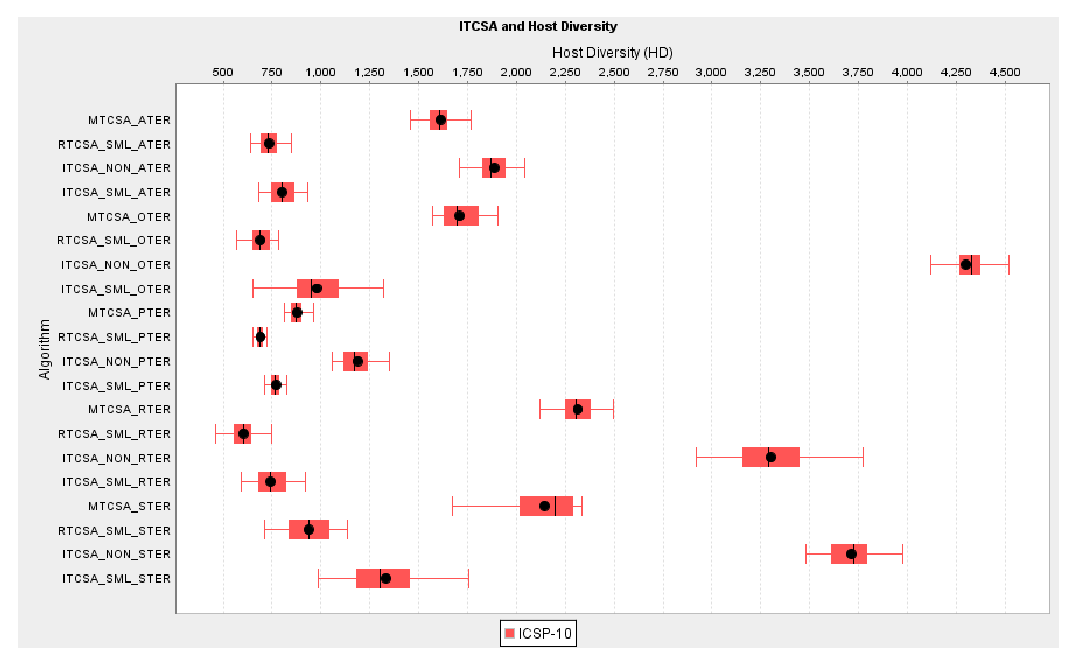
\includegraphics[scale=0.80]{Tissues/ITCSA-HD}
	\caption{Box-and-whisker plot of Host Diversity (HD) across all TER for the ITCSA study.}
	\label{fig:tissues:itcsa:hd:boxplot}
\end{figure}

\begin{figure}[htp]
	\centering
		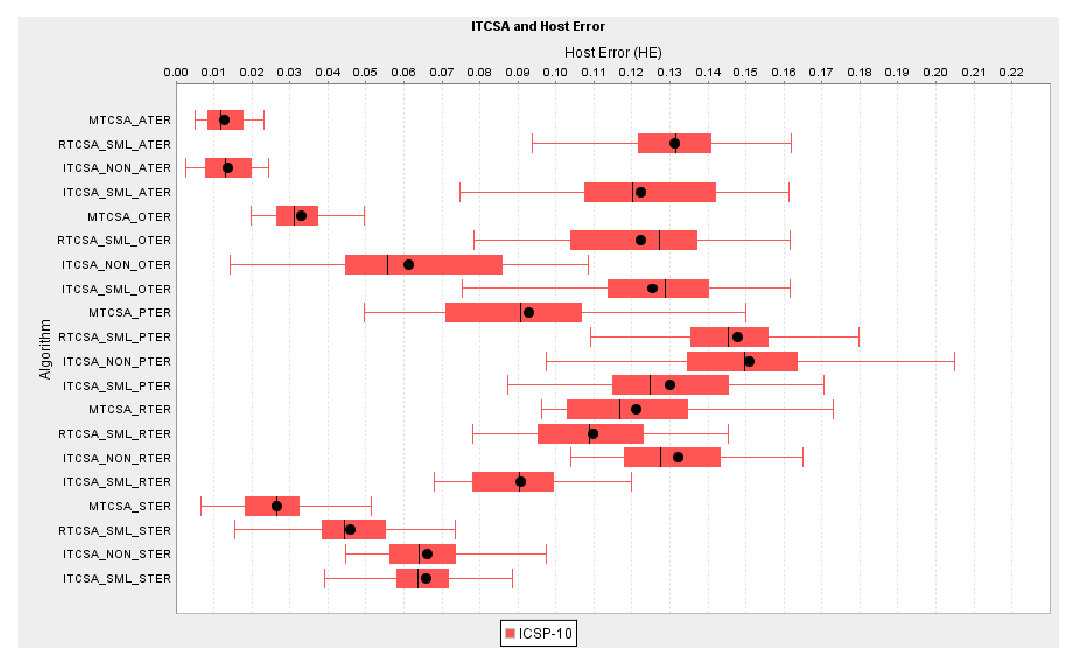
\includegraphics[scale=0.80]{Tissues/ITCSA-HE}
	\caption{Box-and-whisker plot of Host Error (HE) across all TER for the ITCSA study.}
	\label{fig:tissues:itcsa:he:boxplot}
\end{figure}

\begin{figure}[htp]
	\centering
		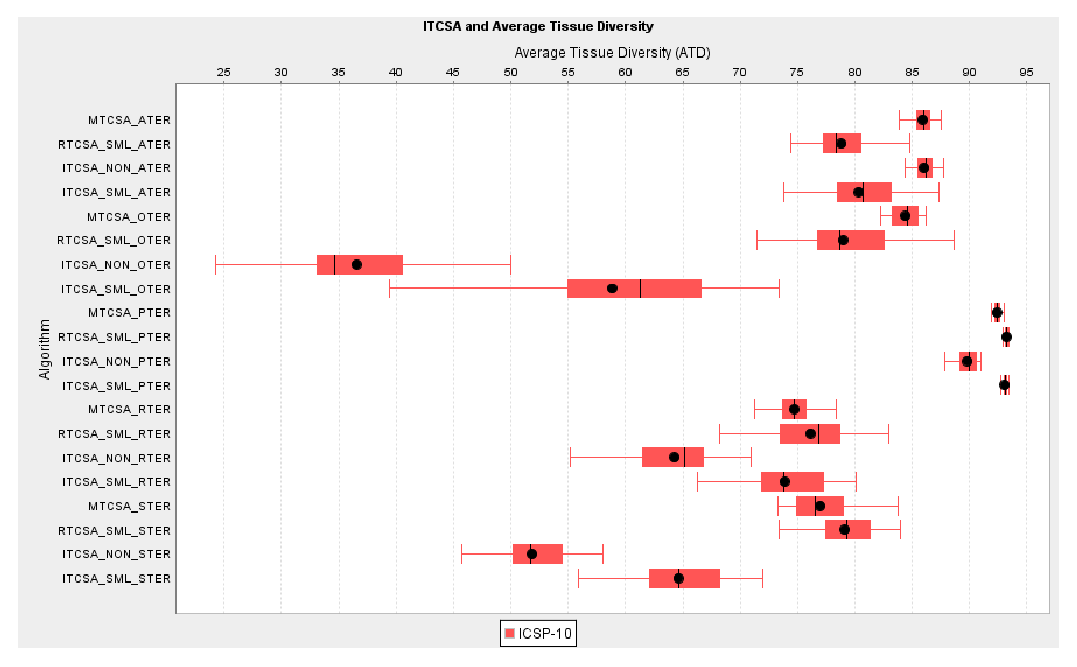
\includegraphics[scale=0.80]{Tissues/ITCSA-ATD}
	\caption{Box-and-whisker plot of Average Tissue Diversity (ATD) across all TER for the ITCSA study.}
	\label{fig:tissues:itcsa:atd:boxplot}
\end{figure}

\begin{figure}[htp]
	\centering
		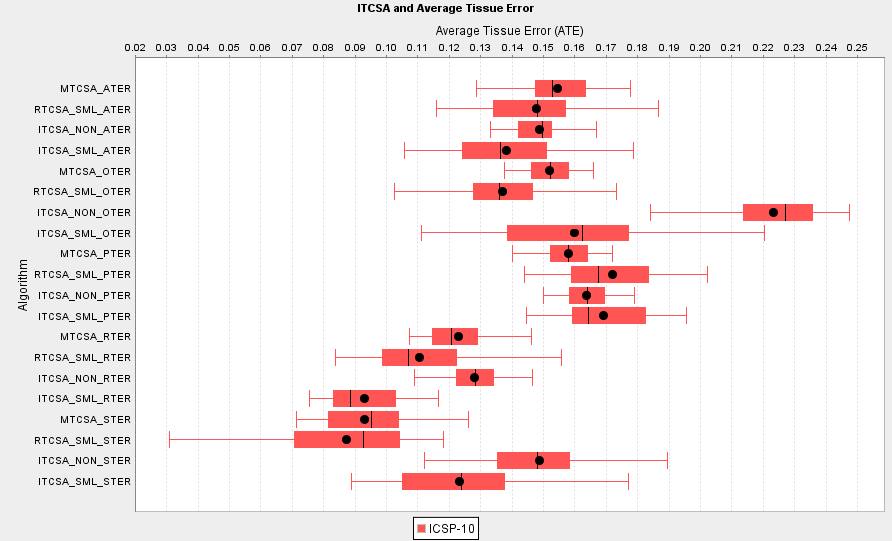
\includegraphics[scale=0.80]{Tissues/ITCSA-ATE}
	\caption{Box-and-whisker plot of Average Tissue Error (ATE) across all TER for the ITCSA study.}
	\label{fig:tissues:itcsa:ate:boxplot}
\end{figure}

%
% Analysis
%
\subsubsection{Analysis}
This section analyses the summarised results in Table~\ref{tab:tissues:itcsa:results} in the context of the aims outlined for this empirical study.

%
% Localisation Trends
% MTCSA vs ITCSA-N
%
\paragraph{Localisation Trends}
% general
This section considers the localisation effects of increasing carrying capacity in ITCSA with out recirculation as compared to MTCSA. 
% system
From a system perspective, ITCSA-N resulted in large increases in diversity compared to MTCSA, an effect expected by a strong localising method (Section~\ref{subsec:tissues:paradigm:method:behaviours}). Unexpected was the concurrent large increases in host error across all exposure regimes. This suggests that the additional resources were exploited by specialising the system, although at the cost of resources that were required for improving the response.
% component
From a component level, ITCSA-N resulted in a general decrease in the average tissue diversity, and a general increase in the average tissue error. This increased tissue internal homogeneity is expected given that increased capacity is exploited by local clonal progeny, although the impaired average tissue capability across the TER's correlates with the systems increase in response error. This suggests that an artefact of the mechanism may be responsible for disrupting the acquisition of information. 
% trends
The observations may be generalised into the following trends:

\begin{enumerate}
	\item Inflammation facilitates component and system level increases in diversity as expected by a strong localising effect.
	\item Inflammation's promise of localisation is broken by the increase in system and component level error, likely an artefact of the specific implementation.
\end{enumerate}

%
% Counter-Disruptive Trends
% RTCSA-S vs ITCSA-S
%
\paragraph{Counter-Disruptive Trends}
This section considers the capability of ITCSA (specifically ITCSA with recirculation: ITCSA-S) to counter the disruptive effects of recirculation to the local exposure regimes such as ATER, OTER and PTER. 
% system
From a system level ITCSA-S resulted in an increase in diversity compared to RTCSA-S, although less a dramatic increase than between ITCSA-N and MTCSA given RTCSA also decrease diversity compared with MTCSA. The diversity increase aligns with the expectation of increased localisation, and with the observation in the previous comparison. ITCSA-S resulted in an increase in error on ATER and STER and a decrease in system error for PTER and RTER over RTCSA-S.
% component
From a component perspective inflammation resulted in a general decrease in the average tissue diversity, with an increase observed on ATER. Component error was increased for OTER and STER, although decreased with inflammation on ATER and RTER.

% trends / inflammation theory
The important finding and confirmation that inflammation can counter the disruptive effects of recirculation is the decrease in HE on PTER and RTER. This finding becomes clear when one considers the global effects of varying carrying capacity with each exposure. In the case of regular system-wide exposure regimes (these are regimes under which each tissue is exposed to some information each host exposure) such as STER and ATER, the carrying capacity for each tissue is always increased to $N_{maxcells}$. For those regimes where regular system-wide exposure is not assured, such as OTER, PTER and RTER, the irregularity promotes variability in the carrying capacity. Given that system error was not decreased for STER and ATER it suggests that the holistic increase in repertoire size does decrease the disruption of recirculation, rather the inflammation provided an effect that increased error on ATER and STER. In the case of PTER and RTER system error was reduced over recirculation suggesting that the variable repertoire sizes across the host and the inflammation mechanisms method for exploiting the extra size (with progeny of selected cells) can only be exploited under these circumstances. 
% component trends
Interestingly inflammation provided some increase and decrease in average per-component error that did not align with the regular and irregular system-wide exposure correlation, and in particular improved average component capability for both the archetype regular and irregular exposure regimes (ATER and RTER). These observations are reduced to the following general trends:

\begin{enumerate}
	\item Inflammation generally counters the disruptive effects of recirculation with regard to system diversity, although system-level benefits are observed only under those exposure regimes that have irregular exposure regimes with regard to the number of tissues exposed to information per host exposure (epoch).	 
	\item Inflammation under consistent system-wide exposure regimes results in a holistic increase in repertoire size that under the ITCSA inflammation mechanism decreases system capability with regard to host error.
\end{enumerate}

%
% Conclusions
%
\subsubsection{Conclusions}
This section summarises the findings of the empirical study into the Inflammation Tissue Clonal Selection Algorithm, in terms of the primitives that were the focus of the study and the expectations that motivated the study.

\begin{enumerate}	
	\item \emph{Inflammation}
	\begin{enumerate}
		\item Inflammation promotes localisation that is apparent with and without recirculation, although it generally disrupts system capability (error).
		\item The increase in carrying capacity mechanisms is only effectively exploited as a counter measure to the disruptive effects of recirculation under exposure regimes that promote disparity in the resulting effect (non-uniform tissue exposure).
	\end{enumerate}
\end{enumerate}

The results suggest at the potential of the emergent effect although raise questions regarding the specifics of the chosen mechanism. Specifically, the method by which increased carrying capacity is exploited (what cells fill the space), and the method by which carrying capacity is decreased (what cells are selected and deleted from the repertoire). It is likely that viable cell lineages are stopped under random cell deletion resulting in the general increase in system error rather than an expected neutrality and potential decreases provided by increase specialisation. An alternative mechanism may be increased progeny tournaments for progeny during integration into the repertoire after creation, providing a natural mechanism for competition for increasingly limited resources. There is much room for elaboration on the primitive realisation of the inflammation effect, not limited to the discussed manipulation of the recirculation effect (increased tissue inflow and decreased tissue outflow), as well as the clear integration of preferential residence retain specialised resources at the point of use (homing).

%
% Summary
% A summary of what the chapter contains, A description of how this leads into the next chapter
%
\section{Chapter Summary}
\label{sec:tissues:summary}

%
% Paradigm Review
%
\subsection{Paradigm Review}
% other attempts
It is important to note that tissue models of the immune system have been considered before by Twycross and Aickelin \cite{Twycross2005} concerned with the innate immune system, and by Bentley, et al. \cite{Bentley2005} concerned with tissue growth models. The principle difference and contribution of the presented approach is the integrated and subsumed relationship with the existing clonal selection paradigm.
% this paradigm
The \emph{Tissue Clonal Selection Paradigm (TCSP)} was defined as the investigation of the cellular clonal selection paradigm as constrained by the concerns of (1) multiple discrete repertoires of cells called \emph{Tissues} and their interactions, and (2) the concerns of regimes of discrete repertoire exposures with information called \emph{Tissue Exposure Regimes (TER)}. The paradigm exploits the metaphor of a holistic immune system called a \emph{Host}, arranged into a lymphatic system of lymphoid tissues that may inter-communicate using the differential trafficking of lymphocyte cells called a \emph{Tissue Clonal Selection Algorithm (TCSA)}. The principle information processing interest of the paradigm as gleamed from the metaphor are the information management strategies that may be employed to address the known and unknown regularities and irregularities in an antigenic \emph{Habitat} of information called an \emph{Infection Antigenic Exposure Problem (ITEP)} toward continuous acquisition of information and the anticipation of needs of acquired information. An abstract foundation for the paradigm was defined in terms of model components, discrete exposures with spatial-temporal regularities, and a series of architectures that may be exploited for arranging the components of tissue models. 


%
% Trends and Findings
%
\subsection{Principles and Findings}
The following summarise the important principles and findings from the definition and investigations into the Tissue Clonal Selection Paradigm:

\paragraph{General Principles}
		\begin{enumerate}
			\item \emph{Natural organisation based on exposure}: Given sufficient time and resources, information is naturally organised in a fixed structured system based on regularity and consistency of its exposure. For example, system-wide exposure naturally promotes system-wide anticipation and point-wise exposure promotes point-wise anticipation.
			\item \emph{Problem is in the exposure regime}: Resources are not always sufficient, therefore information management strategies promote more efficient and effective organisation of information in the face of unknown regularities and irregularities in information exposure and anticipation.
			\item \emph{Strategies based on tissue-level immunology}: The immune system inspires strategies for this problem as the survival of the host relies on the effective acquisition of information and efficient intra-host application of acquired information to fight infections.
		\end{enumerate}

\paragraph{Specific Findings}
		\begin{enumerate}
			\item \emph{Recirculation}: Scope of system exposure (number of tissues) is best addressed with a match in scope of information management strategy at a system level, although the general trend at the component level is invariant to the strategy used. For example the specialisation of response is suitable for regular constrained exposure, whereas the unbiased dissemination is suitable for irregular and/or unconstrained exposure, although such strategies do not counter the general natural component-wise trends in organisation.
			\item \emph{Homing}: The dissemination of information under a constrained exposure regime when such dissemination is unneeded provides a disruptive effect that may be countered by empowering cells to exhibit a preferential residence, whist not impairing dissemination under those regimes that benefit from the effect.
			\item \emph{Inflammation}: The increase in carrying capacity toward decreasing the competition for local resources at those points of the system that are exposed provides a second mechanism for decreasing the disruptive effects of recirculation under those exposure regimes where disparity of the effect is promoted, at the cost of providing a negative effect under those regimes that do not.
		\end{enumerate}	

%
% Paradigm Integration
%
\subsection{Integration}
The \emph{Cellular Clonal Selection Paradigm} defined and investigated in Chapter \ref{chap:cells} was concerned with the adaptation as a method for information acquisition, and the how that method is influenced by degenerate information and inter-cell interactions. The Tissue Clonal Selection Paradigm defined and investigated in this chapter took information acquisition via adaptation for granted, using it as a primitive component in a Tissue Clonal Selection Algorithm raising the level of abstraction regarding information acquisition and adaptation from cells to tissues. The interest in this chapter was how different decentralised information management strategies effected the organisation acquisition and use of information under different information exposure regimes. 
% application
The abstract tissue paradigm is grounded in Chapter~\ref{chap:iidle} in the context of two general problem domains, highlighting the potential benefits the tissue algorithms provide over the cellular clonal selection algorithms.
% next chapter
The subsumption theme of raising the level of abstraction in information processing is continued in Chapter \ref{chap:hosts} in which a Tissue Clonal Selection Algorithm is made a primitive component in a broader \emph{Host Clonal Selection Paradigm} that is concerned with information management strategies in a population of hosts.

% EOF